% Options for packages loaded elsewhere
\PassOptionsToPackage{unicode}{hyperref}
\PassOptionsToPackage{hyphens}{url}
%
\documentclass[
]{article}
\usepackage{amsmath,amssymb}
\usepackage{iftex}
\ifPDFTeX
  \usepackage[T1]{fontenc}
  \usepackage[utf8]{inputenc}
  \usepackage{textcomp} % provide euro and other symbols
\else % if luatex or xetex
  \usepackage{unicode-math} % this also loads fontspec
  \defaultfontfeatures{Scale=MatchLowercase}
  \defaultfontfeatures[\rmfamily]{Ligatures=TeX,Scale=1}
\fi
\usepackage{lmodern}
\ifPDFTeX\else
  % xetex/luatex font selection
\fi
% Use upquote if available, for straight quotes in verbatim environments
\IfFileExists{upquote.sty}{\usepackage{upquote}}{}
\IfFileExists{microtype.sty}{% use microtype if available
  \usepackage[]{microtype}
  \UseMicrotypeSet[protrusion]{basicmath} % disable protrusion for tt fonts
}{}
\makeatletter
\@ifundefined{KOMAClassName}{% if non-KOMA class
  \IfFileExists{parskip.sty}{%
    \usepackage{parskip}
  }{% else
    \setlength{\parindent}{0pt}
    \setlength{\parskip}{6pt plus 2pt minus 1pt}}
}{% if KOMA class
  \KOMAoptions{parskip=half}}
\makeatother
\usepackage{xcolor}
\usepackage[margin=1in]{geometry}
\usepackage{color}
\usepackage{fancyvrb}
\newcommand{\VerbBar}{|}
\newcommand{\VERB}{\Verb[commandchars=\\\{\}]}
\DefineVerbatimEnvironment{Highlighting}{Verbatim}{commandchars=\\\{\}}
% Add ',fontsize=\small' for more characters per line
\usepackage{framed}
\definecolor{shadecolor}{RGB}{248,248,248}
\newenvironment{Shaded}{\begin{snugshade}}{\end{snugshade}}
\newcommand{\AlertTok}[1]{\textcolor[rgb]{0.94,0.16,0.16}{#1}}
\newcommand{\AnnotationTok}[1]{\textcolor[rgb]{0.56,0.35,0.01}{\textbf{\textit{#1}}}}
\newcommand{\AttributeTok}[1]{\textcolor[rgb]{0.13,0.29,0.53}{#1}}
\newcommand{\BaseNTok}[1]{\textcolor[rgb]{0.00,0.00,0.81}{#1}}
\newcommand{\BuiltInTok}[1]{#1}
\newcommand{\CharTok}[1]{\textcolor[rgb]{0.31,0.60,0.02}{#1}}
\newcommand{\CommentTok}[1]{\textcolor[rgb]{0.56,0.35,0.01}{\textit{#1}}}
\newcommand{\CommentVarTok}[1]{\textcolor[rgb]{0.56,0.35,0.01}{\textbf{\textit{#1}}}}
\newcommand{\ConstantTok}[1]{\textcolor[rgb]{0.56,0.35,0.01}{#1}}
\newcommand{\ControlFlowTok}[1]{\textcolor[rgb]{0.13,0.29,0.53}{\textbf{#1}}}
\newcommand{\DataTypeTok}[1]{\textcolor[rgb]{0.13,0.29,0.53}{#1}}
\newcommand{\DecValTok}[1]{\textcolor[rgb]{0.00,0.00,0.81}{#1}}
\newcommand{\DocumentationTok}[1]{\textcolor[rgb]{0.56,0.35,0.01}{\textbf{\textit{#1}}}}
\newcommand{\ErrorTok}[1]{\textcolor[rgb]{0.64,0.00,0.00}{\textbf{#1}}}
\newcommand{\ExtensionTok}[1]{#1}
\newcommand{\FloatTok}[1]{\textcolor[rgb]{0.00,0.00,0.81}{#1}}
\newcommand{\FunctionTok}[1]{\textcolor[rgb]{0.13,0.29,0.53}{\textbf{#1}}}
\newcommand{\ImportTok}[1]{#1}
\newcommand{\InformationTok}[1]{\textcolor[rgb]{0.56,0.35,0.01}{\textbf{\textit{#1}}}}
\newcommand{\KeywordTok}[1]{\textcolor[rgb]{0.13,0.29,0.53}{\textbf{#1}}}
\newcommand{\NormalTok}[1]{#1}
\newcommand{\OperatorTok}[1]{\textcolor[rgb]{0.81,0.36,0.00}{\textbf{#1}}}
\newcommand{\OtherTok}[1]{\textcolor[rgb]{0.56,0.35,0.01}{#1}}
\newcommand{\PreprocessorTok}[1]{\textcolor[rgb]{0.56,0.35,0.01}{\textit{#1}}}
\newcommand{\RegionMarkerTok}[1]{#1}
\newcommand{\SpecialCharTok}[1]{\textcolor[rgb]{0.81,0.36,0.00}{\textbf{#1}}}
\newcommand{\SpecialStringTok}[1]{\textcolor[rgb]{0.31,0.60,0.02}{#1}}
\newcommand{\StringTok}[1]{\textcolor[rgb]{0.31,0.60,0.02}{#1}}
\newcommand{\VariableTok}[1]{\textcolor[rgb]{0.00,0.00,0.00}{#1}}
\newcommand{\VerbatimStringTok}[1]{\textcolor[rgb]{0.31,0.60,0.02}{#1}}
\newcommand{\WarningTok}[1]{\textcolor[rgb]{0.56,0.35,0.01}{\textbf{\textit{#1}}}}
\usepackage{graphicx}
\makeatletter
\def\maxwidth{\ifdim\Gin@nat@width>\linewidth\linewidth\else\Gin@nat@width\fi}
\def\maxheight{\ifdim\Gin@nat@height>\textheight\textheight\else\Gin@nat@height\fi}
\makeatother
% Scale images if necessary, so that they will not overflow the page
% margins by default, and it is still possible to overwrite the defaults
% using explicit options in \includegraphics[width, height, ...]{}
\setkeys{Gin}{width=\maxwidth,height=\maxheight,keepaspectratio}
% Set default figure placement to htbp
\makeatletter
\def\fps@figure{htbp}
\makeatother
\setlength{\emergencystretch}{3em} % prevent overfull lines
\providecommand{\tightlist}{%
  \setlength{\itemsep}{0pt}\setlength{\parskip}{0pt}}
\setcounter{secnumdepth}{-\maxdimen} % remove section numbering
\ifLuaTeX
  \usepackage{selnolig}  % disable illegal ligatures
\fi
\usepackage{bookmark}
\IfFileExists{xurl.sty}{\usepackage{xurl}}{} % add URL line breaks if available
\urlstyle{same}
\hypersetup{
  pdftitle={Build and deploy a stroke prediction model using R},
  pdfauthor={Khadija Musayeva},
  hidelinks,
  pdfcreator={LaTeX via pandoc}}

\title{Build and deploy a stroke prediction model using R}
\author{Khadija Musayeva}
\date{2025-04-05}

\begin{document}
\maketitle

\section{About Data Analysis Report}\label{about-data-analysis-report}

This RMarkdown file contains the report of the data analysis done for
the project on building and deploying a stroke prediction model in R. It
contains analysis such as data exploration, data visualization,
statistical/epidemiological analysis and building the prediction models.
The final report was completed on Sat Apr 5 15:40:16 2025.

\textbf{Data Description:}

According to the World Health Organization (WHO) stroke is the 2nd
leading cause of death globally, responsible for approximately 11\% of
total deaths.

This data set is used to predict whether a patient is likely to get
stroke based on the input parameters like gender, age, various diseases,
and smoking status. Each row in the data provides relevant information
about the patient.

\subsection{Data preprocessing and
analysis}\label{data-preprocessing-and-analysis}

\subsubsection{Install and load
packages}\label{install-and-load-packages}

\begin{Shaded}
\begin{Highlighting}[]
\DocumentationTok{\#\#\# we use pacman to install and load the required packages}
\ControlFlowTok{if}\NormalTok{ (}\SpecialCharTok{!}\FunctionTok{require}\NormalTok{(}\StringTok{"pacman"}\NormalTok{)) }\FunctionTok{install.packages}\NormalTok{(}\StringTok{"pacman"}\NormalTok{)}
\NormalTok{pacman}\SpecialCharTok{::}\FunctionTok{p\_load}\NormalTok{(}\StringTok{"caret"}\NormalTok{, }\StringTok{"data.table"}\NormalTok{, }\StringTok{"DescTools"}\NormalTok{, }\StringTok{"epitools"}\NormalTok{, }\StringTok{"GGally"}\NormalTok{, }\StringTok{"ggplot2"}\NormalTok{, }\StringTok{"gridExtra"}\NormalTok{, }\StringTok{"mlbench"}\NormalTok{, }\StringTok{"mltools"}\NormalTok{, }\StringTok{"naniar"}\NormalTok{, }\StringTok{"parsnip"}\NormalTok{, }\StringTok{"pROC"}\NormalTok{, }\StringTok{"ranger"}\NormalTok{, }\StringTok{"reshape2"}\NormalTok{, }\StringTok{"recipes"}\NormalTok{, }\StringTok{"rsample"}\NormalTok{, }\StringTok{"shiny"}\NormalTok{, }\StringTok{"smotefamily"}\NormalTok{, }\StringTok{"themis"}\NormalTok{,}\StringTok{"tidymodels"}\NormalTok{, }\StringTok{"tune"}\NormalTok{, }\StringTok{"viridis"}\NormalTok{, }\StringTok{"workflows"}\NormalTok{, }\StringTok{"yardstick"}\NormalTok{, }\StringTok{"xgboost"}\NormalTok{)}

\FunctionTok{source}\NormalTok{(}\StringTok{"utils.R"}\NormalTok{)}
\end{Highlighting}
\end{Shaded}

\subsubsection{Load the data}\label{load-the-data}

Read the data and check its dimensions:

\begin{Shaded}
\begin{Highlighting}[]
\NormalTok{dat }\OtherTok{\textless{}{-}} \FunctionTok{as.data.frame}\NormalTok{(}\FunctionTok{read.csv}\NormalTok{(}\StringTok{"healthcare{-}dataset{-}stroke{-}data.csv"}\NormalTok{))}
\FunctionTok{cat}\NormalTok{(}\StringTok{"There are"}\NormalTok{, }\FunctionTok{nrow}\NormalTok{(dat), }\StringTok{"samples and"}\NormalTok{, }\FunctionTok{ncol}\NormalTok{(dat), }\StringTok{"input variables in the stroke data."}\NormalTok{)}
\end{Highlighting}
\end{Shaded}

\begin{verbatim}
## There are 5110 samples and 12 input variables in the stroke data.
\end{verbatim}

What are the types of these variables?

\begin{Shaded}
\begin{Highlighting}[]
\FunctionTok{sapply}\NormalTok{(dat, class)}
\end{Highlighting}
\end{Shaded}

\begin{verbatim}
##                id            gender               age      hypertension 
##         "integer"       "character"         "numeric"         "integer" 
##     heart_disease      ever_married         work_type    Residence_type 
##         "integer"       "character"       "character"       "character" 
## avg_glucose_level               bmi    smoking_status            stroke 
##         "numeric"       "character"       "character"         "integer"
\end{verbatim}

To this end, we can also use str function, it outputs types of column as
well as an overview of some values:

\begin{Shaded}
\begin{Highlighting}[]
\FunctionTok{str}\NormalTok{(dat)}
\end{Highlighting}
\end{Shaded}

\begin{verbatim}
## 'data.frame':    5110 obs. of  12 variables:
##  $ id               : int  9046 51676 31112 60182 1665 56669 53882 10434 27419 60491 ...
##  $ gender           : chr  "Male" "Female" "Male" "Female" ...
##  $ age              : num  67 61 80 49 79 81 74 69 59 78 ...
##  $ hypertension     : int  0 0 0 0 1 0 1 0 0 0 ...
##  $ heart_disease    : int  1 0 1 0 0 0 1 0 0 0 ...
##  $ ever_married     : chr  "Yes" "Yes" "Yes" "Yes" ...
##  $ work_type        : chr  "Private" "Self-employed" "Private" "Private" ...
##  $ Residence_type   : chr  "Urban" "Rural" "Rural" "Urban" ...
##  $ avg_glucose_level: num  229 202 106 171 174 ...
##  $ bmi              : chr  "36.6" "N/A" "32.5" "34.4" ...
##  $ smoking_status   : chr  "formerly smoked" "never smoked" "never smoked" "smokes" ...
##  $ stroke           : int  1 1 1 1 1 1 1 1 1 1 ...
\end{verbatim}

Most of the variables are categorical. We convert them into factor.

\begin{Shaded}
\begin{Highlighting}[]
\NormalTok{dat }\OtherTok{\textless{}{-}}\NormalTok{ dat[, }\SpecialCharTok{{-}}\DecValTok{1}\NormalTok{]}

\NormalTok{dat[, }\SpecialCharTok{{-}}\FunctionTok{c}\NormalTok{(}\DecValTok{2}\NormalTok{, }\DecValTok{8}\NormalTok{, }\DecValTok{9}\NormalTok{)] }\OtherTok{\textless{}{-}} \FunctionTok{lapply}\NormalTok{(dat[, }\SpecialCharTok{{-}}\FunctionTok{c}\NormalTok{(}\DecValTok{2}\NormalTok{, }\DecValTok{8}\NormalTok{, }\DecValTok{9}\NormalTok{)], as.factor)}
  
\NormalTok{dat}\SpecialCharTok{$}\NormalTok{bmi }\OtherTok{\textless{}{-}} \FunctionTok{as.numeric}\NormalTok{(dat}\SpecialCharTok{$}\NormalTok{bmi)}
\end{Highlighting}
\end{Shaded}

Let us have a glimpse of the data:

\begin{Shaded}
\begin{Highlighting}[]
\FunctionTok{head}\NormalTok{(dat)}
\end{Highlighting}
\end{Shaded}

\begin{verbatim}
##   gender age hypertension heart_disease ever_married     work_type
## 1   Male  67            0             1          Yes       Private
## 2 Female  61            0             0          Yes Self-employed
## 3   Male  80            0             1          Yes       Private
## 4 Female  49            0             0          Yes       Private
## 5 Female  79            1             0          Yes Self-employed
## 6   Male  81            0             0          Yes       Private
##   Residence_type avg_glucose_level  bmi  smoking_status stroke
## 1          Urban            228.69 36.6 formerly smoked      1
## 2          Rural            202.21   NA    never smoked      1
## 3          Rural            105.92 32.5    never smoked      1
## 4          Urban            171.23 34.4          smokes      1
## 5          Rural            174.12 24.0    never smoked      1
## 6          Urban            186.21 29.0 formerly smoked      1
\end{verbatim}

\subsubsection{\texorpdfstring{\textbf{Analysis of missing
values}}{Analysis of missing values}}\label{analysis-of-missing-values}

To analyze the missing values we use naniar package. The following plot
shows that 4 percent of bmi values, or 201 of observations have bmi
values missing.

\begin{Shaded}
\begin{Highlighting}[]
\FunctionTok{vis\_miss}\NormalTok{(dat)}
\end{Highlighting}
\end{Shaded}

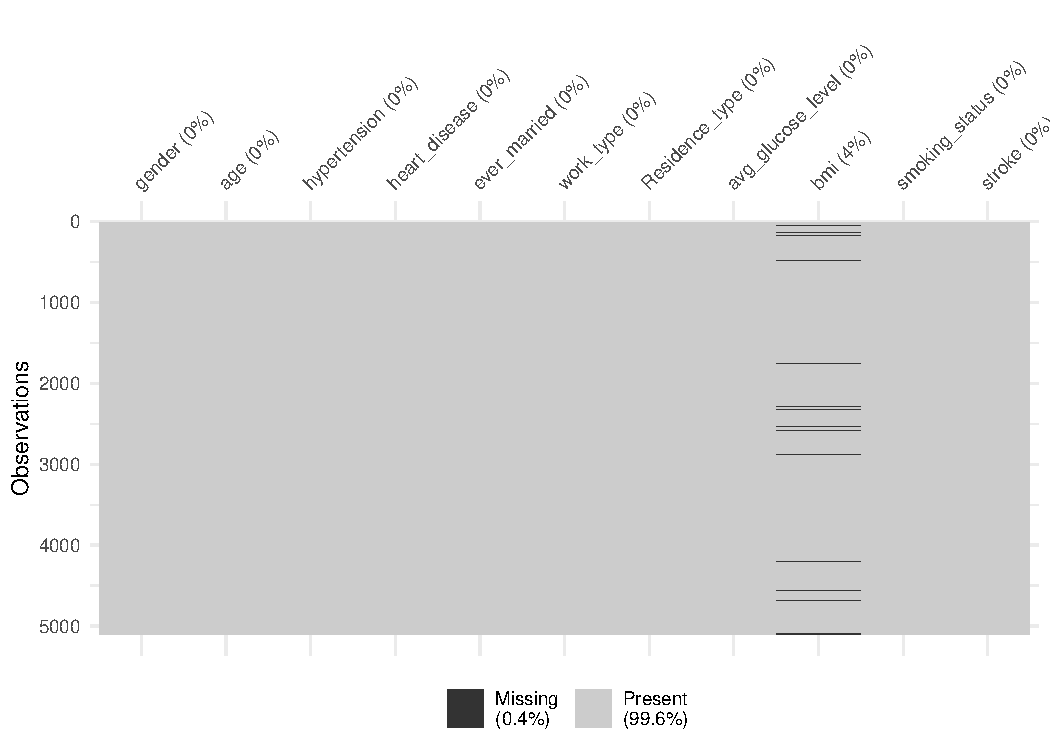
\includegraphics{Build-deploy-stroke-prediction-model-R_files/figure-latex/miss-plot-1.pdf}

Are these missing values distributed randomly? To this end, we look at
the distribution of missing values with respect to the variables of
interest. For instance, regarding gender, there are more missing values
for males than for females, and regarding the output variable of
interest, almost \textasciitilde16 percent of BMI values for stroke
individuals are missing which is at most 4 percent for non-stroke
individuals. So these values are missing at random.

\begin{Shaded}
\begin{Highlighting}[]
\NormalTok{p1 }\OtherTok{\textless{}{-}} \FunctionTok{plot\_missingness\_distribution}\NormalTok{(dat, }\StringTok{"gender"}\NormalTok{)}

\NormalTok{p2 }\OtherTok{\textless{}{-}} \FunctionTok{plot\_missingness\_distribution}\NormalTok{(dat, }\StringTok{"stroke"}\NormalTok{)}

\FunctionTok{grid.arrange}\NormalTok{(p1, p2, }\AttributeTok{ncol =} \DecValTok{2}\NormalTok{)}
\end{Highlighting}
\end{Shaded}

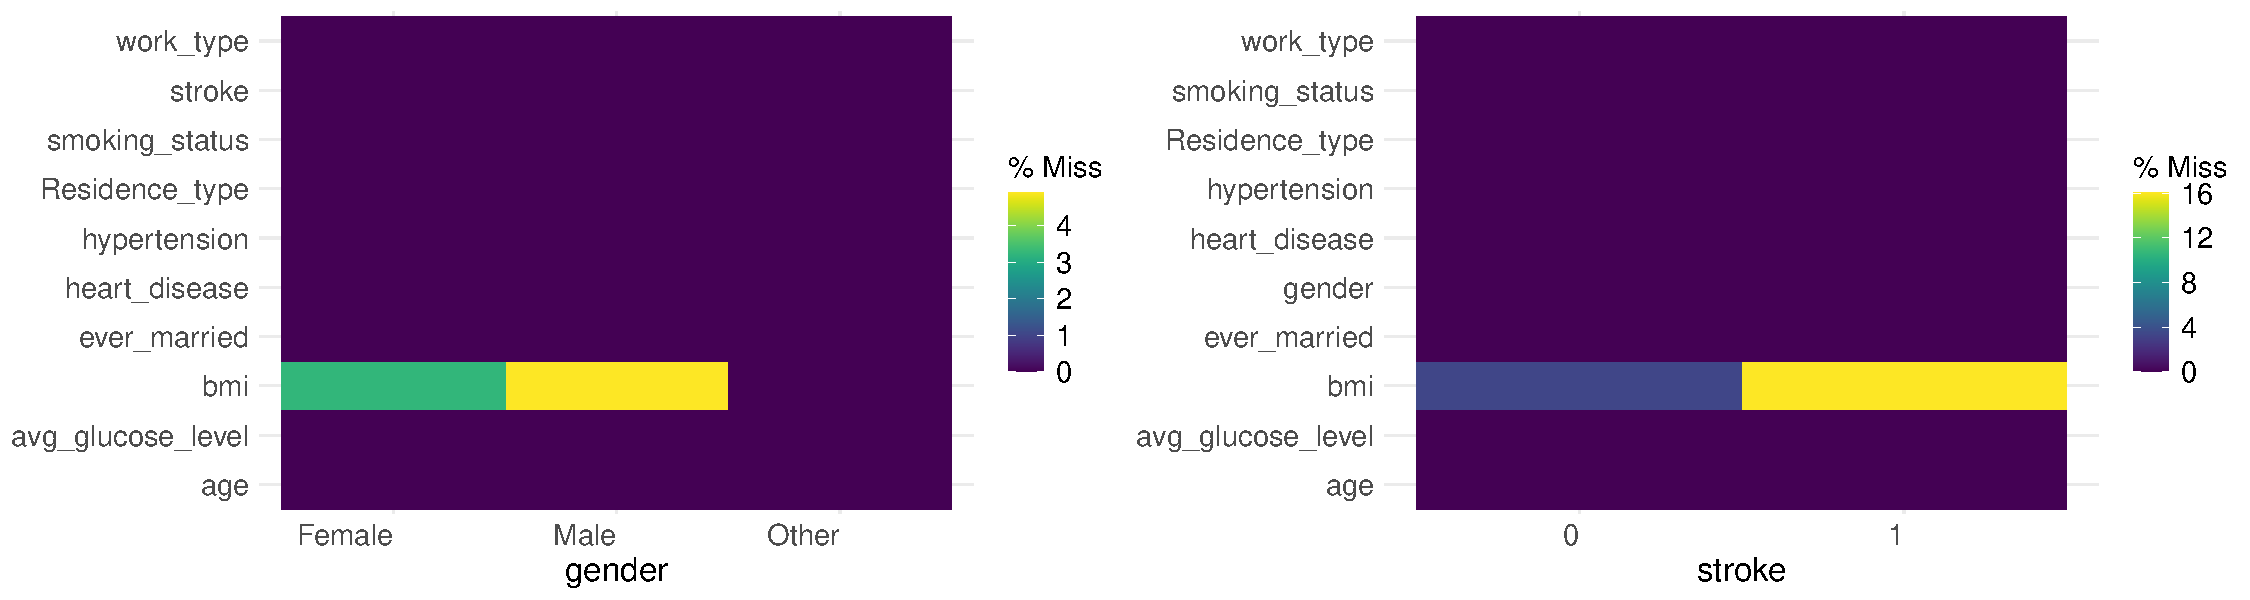
\includegraphics{Build-deploy-stroke-prediction-model-R_files/figure-latex/miss-distribution-plot-1.pdf}

\subsubsection{\texorpdfstring{\textbf{Visualization}}{Visualization}}\label{visualization}

The following plots show the distribution of categorical variables.

\begin{Shaded}
\begin{Highlighting}[]
\CommentTok{\# Select categorical variables and stroke column}
\NormalTok{cat\_vars }\OtherTok{\textless{}{-}}\NormalTok{ dat[, }\SpecialCharTok{{-}}\FunctionTok{c}\NormalTok{(}\DecValTok{2}\NormalTok{, }\DecValTok{8}\NormalTok{, }\DecValTok{9}\NormalTok{)]}
\NormalTok{stroke }\OtherTok{\textless{}{-}}\NormalTok{ dat}\SpecialCharTok{$}\NormalTok{stroke}

\CommentTok{\# convert into long format}
\NormalTok{long\_dat }\OtherTok{\textless{}{-}}\NormalTok{ cat\_vars }\SpecialCharTok{\%\textgreater{}\%} \FunctionTok{pivot\_longer}\NormalTok{(}\AttributeTok{cols =} \FunctionTok{everything}\NormalTok{(), }\AttributeTok{names\_to =} \StringTok{"variable"}\NormalTok{, }\AttributeTok{values\_to =} \StringTok{"value"}\NormalTok{)}

\CommentTok{\# change the order of categorical variables for plot}
\NormalTok{long\_dat}\SpecialCharTok{$}\NormalTok{variable }\OtherTok{\textless{}{-}} \FunctionTok{factor}\NormalTok{(long\_dat}\SpecialCharTok{$}\NormalTok{variable, }\AttributeTok{levels =} \FunctionTok{c}\NormalTok{(}\StringTok{"stroke"}\NormalTok{, }\StringTok{"gender"}\NormalTok{, }\StringTok{"hypertension"}\NormalTok{,  }\StringTok{"heart\_disease"}\NormalTok{, }\StringTok{"smoking\_status"}\NormalTok{, }\StringTok{"ever\_married"}\NormalTok{, }\StringTok{"work\_type"}\NormalTok{, }\StringTok{"Residence\_type"}\NormalTok{)) }

\CommentTok{\# bar plot of percentages}
\FunctionTok{ggplot}\NormalTok{(long\_dat, }\FunctionTok{aes}\NormalTok{(}\AttributeTok{x =}\NormalTok{ value, }\AttributeTok{y =} \FunctionTok{after\_stat}\NormalTok{(prop), }\AttributeTok{fill=}\NormalTok{variable)) }\SpecialCharTok{+}
  \FunctionTok{geom\_bar}\NormalTok{(}\AttributeTok{position =} \FunctionTok{position\_dodge}\NormalTok{(), }\AttributeTok{stat =} \StringTok{"prop"}\NormalTok{)}\SpecialCharTok{+}
  \FunctionTok{geom\_text}\NormalTok{(}\FunctionTok{aes}\NormalTok{(}\AttributeTok{label =} \FunctionTok{round}\NormalTok{(}\DecValTok{100} \SpecialCharTok{*} \FunctionTok{after\_stat}\NormalTok{(prop), }\DecValTok{2}\NormalTok{)),}
    \AttributeTok{position =} \FunctionTok{position\_dodge}\NormalTok{(.}\DecValTok{9}\NormalTok{), }\AttributeTok{stat =} \StringTok{"prop"}\NormalTok{, }\AttributeTok{vjust =} \SpecialCharTok{{-}}\NormalTok{.}\DecValTok{2}
\NormalTok{  ) }\SpecialCharTok{+} 
  \FunctionTok{facet\_wrap}\NormalTok{(}\SpecialCharTok{\textasciitilde{}}\NormalTok{ variable, }\AttributeTok{nrow =} \DecValTok{2}\NormalTok{, }\AttributeTok{ncol =} \DecValTok{4}\NormalTok{, }\AttributeTok{scales =} \StringTok{"free\_x"}\NormalTok{) }\SpecialCharTok{+}
  \FunctionTok{scale\_fill\_brewer}\NormalTok{(}\AttributeTok{palette =} \StringTok{"Set2"}\NormalTok{) }\SpecialCharTok{+}
  \FunctionTok{theme\_minimal}\NormalTok{(}\AttributeTok{base\_size =} \DecValTok{14}\NormalTok{) }\SpecialCharTok{+}
  \FunctionTok{theme}\NormalTok{(}
    \AttributeTok{plot.title =} \FunctionTok{element\_text}\NormalTok{(}\AttributeTok{hjust =} \FloatTok{0.5}\NormalTok{, }\AttributeTok{size =} \DecValTok{16}\NormalTok{),}
    \AttributeTok{axis.text.x =} \FunctionTok{element\_text}\NormalTok{(}\AttributeTok{angle =} \DecValTok{45}\NormalTok{, }\AttributeTok{hjust =} \DecValTok{1}\NormalTok{),}
    \AttributeTok{strip.text =} \FunctionTok{element\_text}\NormalTok{(}\AttributeTok{size =} \DecValTok{12}\NormalTok{),}
    \AttributeTok{panel.spacing =} \FunctionTok{unit}\NormalTok{(}\FloatTok{1.2}\NormalTok{, }\StringTok{"lines"}\NormalTok{),}
    \AttributeTok{legend.position=}\StringTok{"none"}
\NormalTok{  ) }\SpecialCharTok{+}
  \FunctionTok{labs}\NormalTok{(}
    \AttributeTok{x =} \StringTok{""}\NormalTok{,}
    \AttributeTok{y =} \StringTok{"Proportion of observations"}\NormalTok{,}
    \AttributeTok{title =} \StringTok{""}
\NormalTok{  )}
\end{Highlighting}
\end{Shaded}

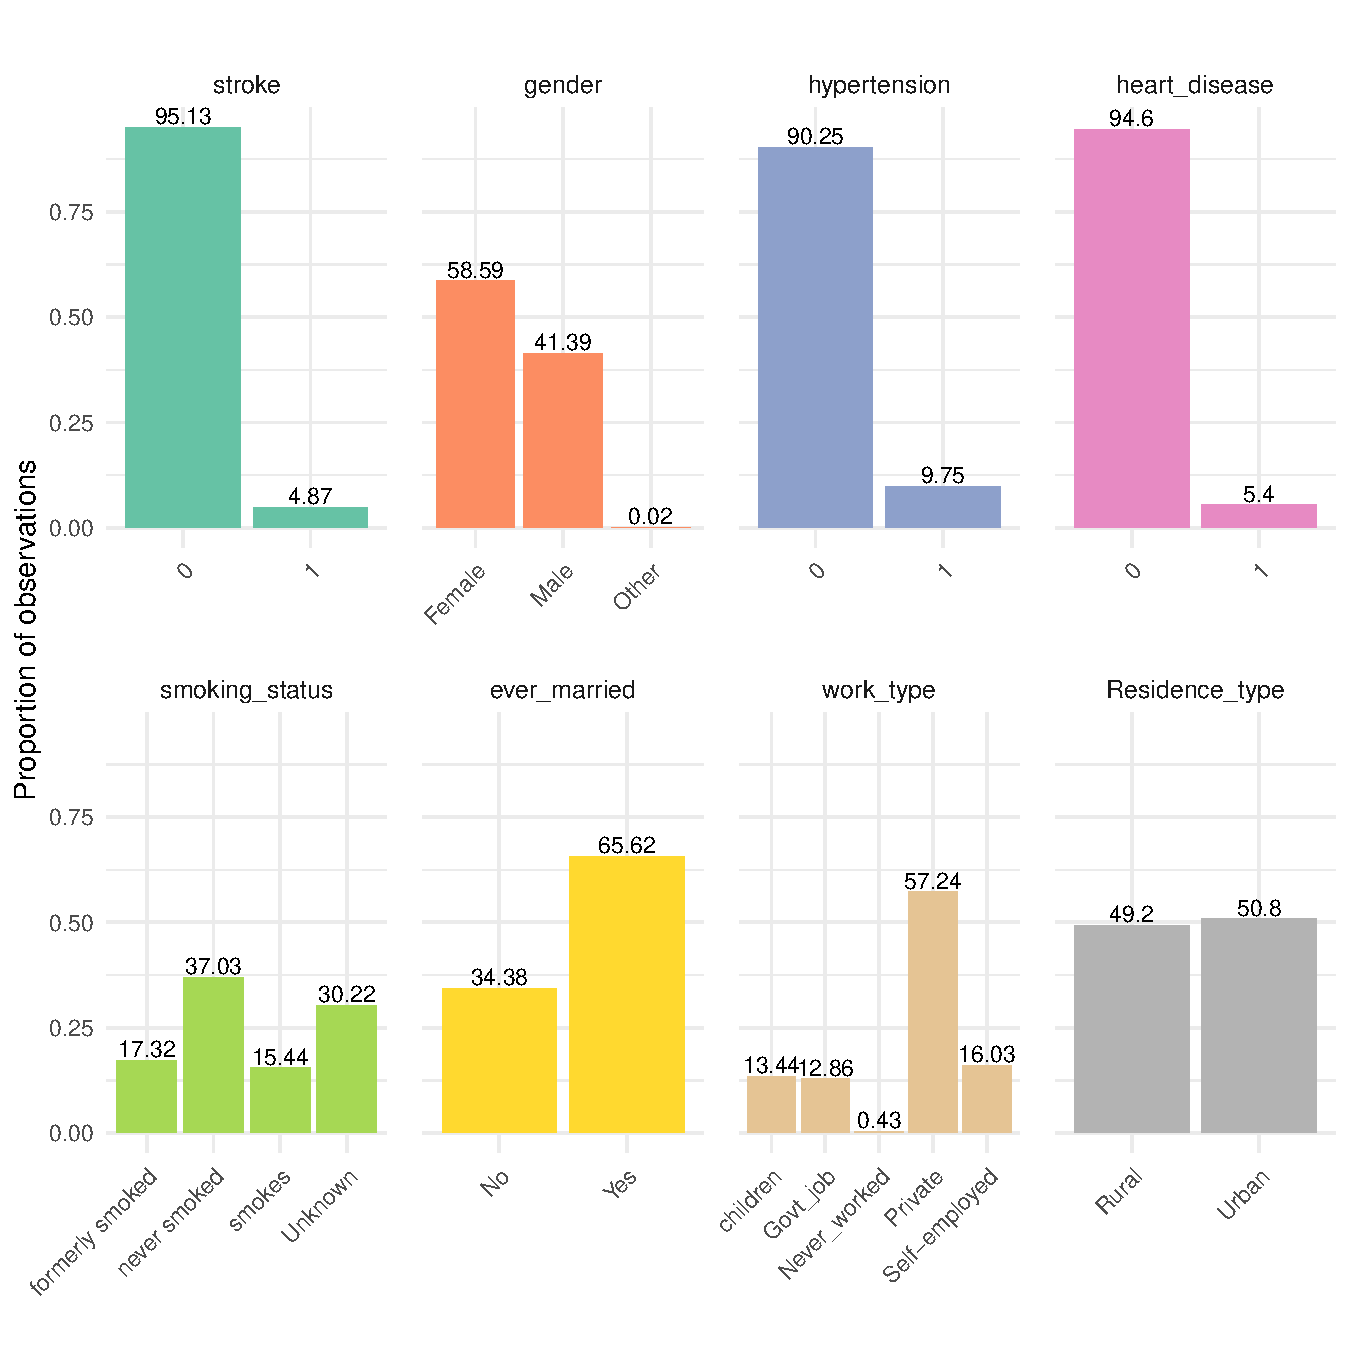
\includegraphics{Build-deploy-stroke-prediction-model-R_files/figure-latex/cat-plot-1.pdf}

We see that in this study there are more females than males, more
individuals with positive ever-married status, more individuals working
in the private sector than the remaining sectors. There are almost the
same number of observations in rural and urban categories. Below we look
at the prevalence of stroke cases across all categorical variables.

\begin{Shaded}
\begin{Highlighting}[]
\NormalTok{cat\_vars }\OtherTok{\textless{}{-}}\NormalTok{ dat[, }\SpecialCharTok{{-}}\FunctionTok{c}\NormalTok{(}\DecValTok{2}\NormalTok{, }\DecValTok{8}\NormalTok{, }\DecValTok{9}\NormalTok{, }\DecValTok{11}\NormalTok{)]  }\CommentTok{\# remove continuous vars or unwanted cols}
\NormalTok{cat\_vars}\SpecialCharTok{$}\NormalTok{stroke }\OtherTok{\textless{}{-}}\NormalTok{ dat}\SpecialCharTok{$}\NormalTok{stroke  }\CommentTok{\# keep stroke indicator}

\CommentTok{\# convert to long format}
\NormalTok{long\_dat }\OtherTok{\textless{}{-}}\NormalTok{ cat\_vars }\SpecialCharTok{\%\textgreater{}\%}
  \FunctionTok{pivot\_longer}\NormalTok{(}\AttributeTok{cols =} \SpecialCharTok{{-}}\NormalTok{stroke, }\AttributeTok{names\_to =} \StringTok{"variable"}\NormalTok{, }\AttributeTok{values\_to =} \StringTok{"value"}\NormalTok{)}

\CommentTok{\# stroke prevalence per category}
\NormalTok{stroke\_pct }\OtherTok{\textless{}{-}}\NormalTok{ long\_dat }\SpecialCharTok{\%\textgreater{}\%}
  \FunctionTok{group\_by}\NormalTok{(variable, value) }\SpecialCharTok{\%\textgreater{}\%}
  \FunctionTok{summarise}\NormalTok{(}
    \AttributeTok{total =} \FunctionTok{n}\NormalTok{(),}
    \AttributeTok{stroke\_cases =} \FunctionTok{sum}\NormalTok{(stroke }\SpecialCharTok{==} \DecValTok{1}\NormalTok{),}
    \AttributeTok{pct =} \FunctionTok{round}\NormalTok{(}\DecValTok{100} \SpecialCharTok{*}\NormalTok{ stroke\_cases }\SpecialCharTok{/}\NormalTok{ total, }\DecValTok{2}\NormalTok{),}
    \AttributeTok{.groups =} \StringTok{"drop"}
\NormalTok{  )}

\CommentTok{\# set the plot order}
\NormalTok{stroke\_pct}\SpecialCharTok{$}\NormalTok{variable }\OtherTok{\textless{}{-}} \FunctionTok{factor}\NormalTok{(stroke\_pct}\SpecialCharTok{$}\NormalTok{variable,}
                              \AttributeTok{levels =} \FunctionTok{c}\NormalTok{(}\StringTok{"gender"}\NormalTok{, }\StringTok{"hypertension"}\NormalTok{, }\StringTok{"heart\_disease"}\NormalTok{,}
                                         \StringTok{"smoking\_status"}\NormalTok{, }\StringTok{"ever\_married"}\NormalTok{,}
                                         \StringTok{"work\_type"}\NormalTok{, }\StringTok{"Residence\_type"}\NormalTok{))}


\FunctionTok{ggplot}\NormalTok{(stroke\_pct, }\FunctionTok{aes}\NormalTok{(}\AttributeTok{x =}\NormalTok{ value, }\AttributeTok{y =}\NormalTok{ pct, }\AttributeTok{fill =}\NormalTok{ variable)) }\SpecialCharTok{+}
  \FunctionTok{geom\_bar}\NormalTok{(}\AttributeTok{stat =} \StringTok{"identity"}\NormalTok{) }\SpecialCharTok{+}
  \FunctionTok{facet\_wrap}\NormalTok{(}\SpecialCharTok{\textasciitilde{}}\NormalTok{variable, }\AttributeTok{nrow =} \DecValTok{2}\NormalTok{, }\AttributeTok{ncol =} \DecValTok{4}\NormalTok{, }\AttributeTok{scales =} \StringTok{"free\_x"}\NormalTok{) }\SpecialCharTok{+}
  \FunctionTok{scale\_fill\_brewer}\NormalTok{(}\AttributeTok{palette =} \StringTok{"Set2"}\NormalTok{) }\SpecialCharTok{+}
  \FunctionTok{theme\_minimal}\NormalTok{(}\AttributeTok{base\_size =} \DecValTok{14}\NormalTok{) }\SpecialCharTok{+}
  \FunctionTok{theme}\NormalTok{(}\AttributeTok{plot.title =} \FunctionTok{element\_text}\NormalTok{(}\AttributeTok{hjust =} \FloatTok{0.5}\NormalTok{, }\AttributeTok{size =} \DecValTok{16}\NormalTok{),}
        \AttributeTok{axis.text.x =} \FunctionTok{element\_text}\NormalTok{(}\AttributeTok{angle =} \DecValTok{45}\NormalTok{, }\AttributeTok{hjust =} \DecValTok{1}\NormalTok{),}
        \AttributeTok{panel.spacing =} \FunctionTok{unit}\NormalTok{(}\FloatTok{1.2}\NormalTok{, }\StringTok{"lines"}\NormalTok{),}
        \AttributeTok{legend.position =} \StringTok{"none"}\NormalTok{) }\SpecialCharTok{+}
  \FunctionTok{labs}\NormalTok{(}\AttributeTok{x =} \StringTok{""}\NormalTok{, }\AttributeTok{y =} \StringTok{"Stroke rate (\%)"}\NormalTok{, }\AttributeTok{title =} \StringTok{""}\NormalTok{)}
\end{Highlighting}
\end{Shaded}

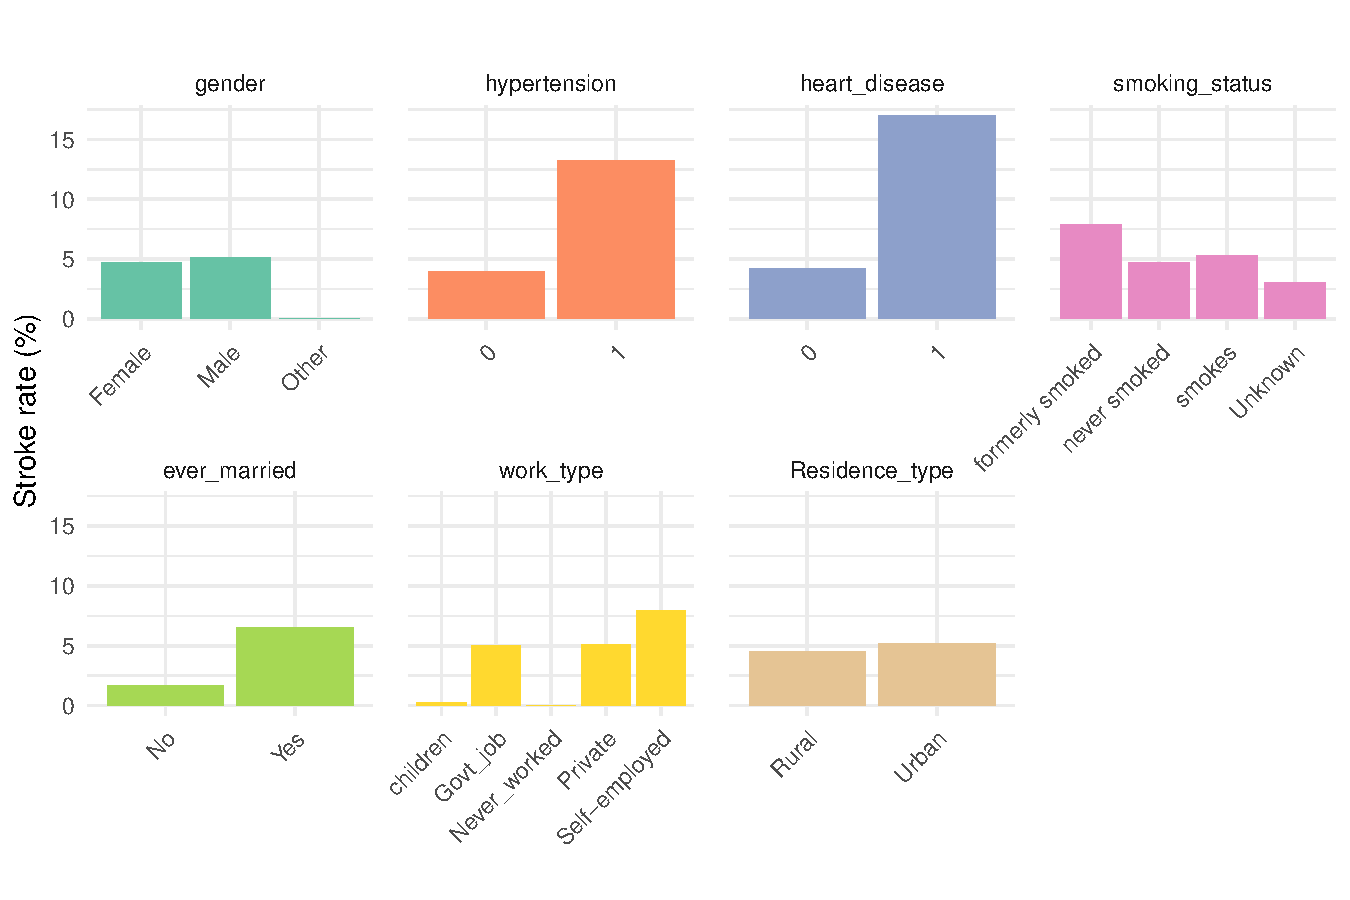
\includegraphics{Build-deploy-stroke-prediction-model-R_files/figure-latex/stroke-plot-1.pdf}

We see that both females and males are equally affected by this medical
condition. There are more stroke cases among individuals with
hypertension, and heart disease. More formerly-smoked individuals have
stroke than the rest, however, there are a lot of individuals with the
unknown smoking status, which makes this analysis biased. In general
these variables are related to the age. For instance, more
formerly-smoked individuals, or ever-married individuals are older
people.

We use \textbf{Cramer's V} to measure associations between multiple
categories. It ranges from 0 (no association) to 1 (perfect
association). The following heatmap shows that there is some association
between smoking status and marriage status, smoking status and work
type. This is likely due to the age of individuals as a confounding
variable. Most of the associations, however, are weak.

\begin{Shaded}
\begin{Highlighting}[]
\NormalTok{cat\_vars }\OtherTok{\textless{}{-}}\NormalTok{ dat[, }\SpecialCharTok{{-}}\FunctionTok{c}\NormalTok{(}\DecValTok{2}\NormalTok{, }\DecValTok{8}\NormalTok{, }\DecValTok{9}\NormalTok{, }\DecValTok{11}\NormalTok{)] }\SpecialCharTok{\%\textgreater{}\%}
  \FunctionTok{mutate}\NormalTok{(}\FunctionTok{across}\NormalTok{(}\FunctionTok{everything}\NormalTok{(), }\SpecialCharTok{\textasciitilde{}} \FunctionTok{droplevels}\NormalTok{(}\FunctionTok{as.factor}\NormalTok{(.))))}

\NormalTok{cramerV\_matrix }\OtherTok{\textless{}{-}} \FunctionTok{compute\_cramer\_v\_matrix}\NormalTok{(cat\_vars)}

\NormalTok{cramerV\_tidy }\OtherTok{\textless{}{-}} \FunctionTok{melt}\NormalTok{(cramerV\_matrix, }\AttributeTok{na.rm =} \ConstantTok{TRUE}\NormalTok{)}

\NormalTok{cramerV\_tidy}\SpecialCharTok{$}\NormalTok{Var1 }\OtherTok{\textless{}{-}} \FunctionTok{factor}\NormalTok{(cramerV\_tidy}\SpecialCharTok{$}\NormalTok{Var1, }\AttributeTok{levels =} \FunctionTok{rownames}\NormalTok{(cramerV\_matrix))}

\NormalTok{cramerV\_tidy}\SpecialCharTok{$}\NormalTok{Var2 }\OtherTok{\textless{}{-}} \FunctionTok{factor}\NormalTok{(cramerV\_tidy}\SpecialCharTok{$}\NormalTok{Var2, }\AttributeTok{levels =} \FunctionTok{colnames}\NormalTok{(cramerV\_matrix))}


\FunctionTok{ggplot}\NormalTok{(cramerV\_tidy, }\FunctionTok{aes}\NormalTok{(Var1, Var2, }\AttributeTok{fill =}\NormalTok{ value)) }\SpecialCharTok{+}
  \FunctionTok{geom\_tile}\NormalTok{(}\AttributeTok{color =} \StringTok{"white"}\NormalTok{) }\SpecialCharTok{+}
  \FunctionTok{scale\_fill\_gradient2}\NormalTok{(}
    \AttributeTok{low =} \StringTok{"white"}\NormalTok{, }\AttributeTok{mid =} \StringTok{"lightblue"}\NormalTok{, }\AttributeTok{high =} \StringTok{"steelblue"}\NormalTok{,}
    \AttributeTok{midpoint =} \FloatTok{0.2}\NormalTok{, }\AttributeTok{limits =} \FunctionTok{c}\NormalTok{(}\DecValTok{0}\NormalTok{, }\DecValTok{1}\NormalTok{), }\AttributeTok{name =} \StringTok{"Cramér’s V"}
\NormalTok{  ) }\SpecialCharTok{+}
  \FunctionTok{geom\_text}\NormalTok{(}\FunctionTok{aes}\NormalTok{(}\AttributeTok{label =} \FunctionTok{round}\NormalTok{(value, }\DecValTok{2}\NormalTok{)), }\AttributeTok{color =} \StringTok{"black"}\NormalTok{, }\AttributeTok{size =} \DecValTok{3}\NormalTok{) }\SpecialCharTok{+}
  \FunctionTok{theme\_minimal}\NormalTok{(}\AttributeTok{base\_size =} \DecValTok{14}\NormalTok{) }\SpecialCharTok{+}
  \FunctionTok{theme}\NormalTok{(}
    \AttributeTok{axis.text.x =} \FunctionTok{element\_text}\NormalTok{(}\AttributeTok{angle =} \DecValTok{45}\NormalTok{, }\AttributeTok{hjust =} \DecValTok{1}\NormalTok{),}
    \AttributeTok{panel.grid =} \FunctionTok{element\_blank}\NormalTok{()}
\NormalTok{  ) }\SpecialCharTok{+}
  \FunctionTok{labs}\NormalTok{(}\AttributeTok{title =} \StringTok{""}\NormalTok{, }\AttributeTok{x =} \StringTok{""}\NormalTok{, }\AttributeTok{y =} \StringTok{""}\NormalTok{ )}
\end{Highlighting}
\end{Shaded}

\begin{verbatim}
## Warning in grid.Call(C_textBounds, as.graphicsAnnot(x$label), x$x, x$y, :
## erreur de conversion de 'Cramér’s V' dans 'mbcsToSbcs' : le point est substitué
## pour <e2>
\end{verbatim}

\begin{verbatim}
## Warning in grid.Call(C_textBounds, as.graphicsAnnot(x$label), x$x, x$y, :
## erreur de conversion de 'Cramér’s V' dans 'mbcsToSbcs' : le point est substitué
## pour <80>
\end{verbatim}

\begin{verbatim}
## Warning in grid.Call(C_textBounds, as.graphicsAnnot(x$label), x$x, x$y, :
## erreur de conversion de 'Cramér’s V' dans 'mbcsToSbcs' : le point est substitué
## pour <99>
\end{verbatim}

\begin{verbatim}
## Warning in grid.Call(C_textBounds, as.graphicsAnnot(x$label), x$x, x$y, :
## erreur de conversion de 'Cramér’s V' dans 'mbcsToSbcs' : le point est substitué
## pour <e2>
\end{verbatim}

\begin{verbatim}
## Warning in grid.Call(C_textBounds, as.graphicsAnnot(x$label), x$x, x$y, :
## erreur de conversion de 'Cramér’s V' dans 'mbcsToSbcs' : le point est substitué
## pour <80>
\end{verbatim}

\begin{verbatim}
## Warning in grid.Call(C_textBounds, as.graphicsAnnot(x$label), x$x, x$y, :
## erreur de conversion de 'Cramér’s V' dans 'mbcsToSbcs' : le point est substitué
## pour <99>
\end{verbatim}

\begin{verbatim}
## Warning in grid.Call.graphics(C_text, as.graphicsAnnot(x$label), x$x, x$y, :
## erreur de conversion de 'Cramér’s V' dans 'mbcsToSbcs' : le point est substitué
## pour <e2>
\end{verbatim}

\begin{verbatim}
## Warning in grid.Call.graphics(C_text, as.graphicsAnnot(x$label), x$x, x$y, :
## erreur de conversion de 'Cramér’s V' dans 'mbcsToSbcs' : le point est substitué
## pour <80>
\end{verbatim}

\begin{verbatim}
## Warning in grid.Call.graphics(C_text, as.graphicsAnnot(x$label), x$x, x$y, :
## erreur de conversion de 'Cramér’s V' dans 'mbcsToSbcs' : le point est substitué
## pour <99>
\end{verbatim}

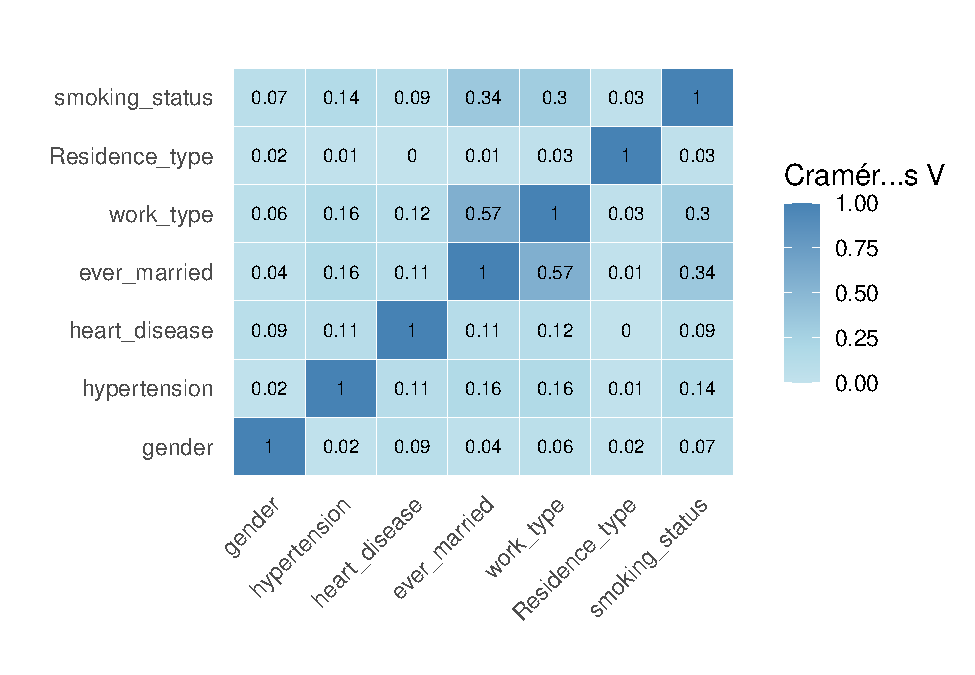
\includegraphics{Build-deploy-stroke-prediction-model-R_files/figure-latex/unnamed-chunk-7-1.pdf}

What about continuous variables: age, average glucose level, and body
mass index?

The majority of individuals have an average glucose level below 150, but
there is a small group of individuals whose average glucose level is
concentrated around \textasciitilde210.

\begin{Shaded}
\begin{Highlighting}[]
\NormalTok{p1 }\OtherTok{\textless{}{-}} \FunctionTok{ggplot}\NormalTok{(dat, }\FunctionTok{aes}\NormalTok{(}\AttributeTok{x=}\NormalTok{avg\_glucose\_level)) }\SpecialCharTok{+}  
      \FunctionTok{geom\_histogram}\NormalTok{(}\AttributeTok{fill=}\StringTok{"\#92C5DE"}\NormalTok{)}\SpecialCharTok{+}
      \FunctionTok{labs}\NormalTok{(}\AttributeTok{x =} \StringTok{"Average glucose level"}\NormalTok{, }\AttributeTok{y =} \StringTok{""}\NormalTok{) }\SpecialCharTok{+}
      \FunctionTok{theme\_minimal}\NormalTok{(}\AttributeTok{base\_size =} \DecValTok{12}\NormalTok{)}\SpecialCharTok{+}
      \FunctionTok{theme}\NormalTok{(}\AttributeTok{legend.position=}\StringTok{"none"}\NormalTok{)}


\NormalTok{p2 }\OtherTok{\textless{}{-}} \FunctionTok{ggplot}\NormalTok{(dat, }\FunctionTok{aes}\NormalTok{(}\AttributeTok{x=}\NormalTok{bmi)) }\SpecialCharTok{+}  
      \FunctionTok{geom\_histogram}\NormalTok{(}\AttributeTok{fill=}\StringTok{"\#E69F00"}\NormalTok{)}\SpecialCharTok{+}
      \FunctionTok{labs}\NormalTok{(}\AttributeTok{x =} \StringTok{"Body mass index"}\NormalTok{, }\AttributeTok{y =} \StringTok{""}\NormalTok{) }\SpecialCharTok{+}
      \FunctionTok{theme\_minimal}\NormalTok{(}\AttributeTok{base\_size =} \DecValTok{12}\NormalTok{)}\SpecialCharTok{+}
      \FunctionTok{theme}\NormalTok{(}\AttributeTok{legend.position=}\StringTok{"none"}\NormalTok{)}


\NormalTok{p3 }\OtherTok{\textless{}{-}} \FunctionTok{ggplot}\NormalTok{(dat, }\FunctionTok{aes}\NormalTok{(}\AttributeTok{x=}\NormalTok{age)) }\SpecialCharTok{+}  
      \FunctionTok{geom\_histogram}\NormalTok{(}\AttributeTok{fill=}\StringTok{"\#D6604D"}\NormalTok{)}\SpecialCharTok{+}
      \FunctionTok{labs}\NormalTok{(}\AttributeTok{x =} \StringTok{"Age"}\NormalTok{, }\AttributeTok{y =} \StringTok{""}\NormalTok{) }\SpecialCharTok{+}
      \FunctionTok{theme\_minimal}\NormalTok{(}\AttributeTok{base\_size =} \DecValTok{12}\NormalTok{)}\SpecialCharTok{+}
      \FunctionTok{theme}\NormalTok{(}\AttributeTok{legend.position=}\StringTok{"none"}\NormalTok{)}


\FunctionTok{grid.arrange}\NormalTok{(p1, p2, p3, }\AttributeTok{ncol=}\DecValTok{3}\NormalTok{)}
\end{Highlighting}
\end{Shaded}

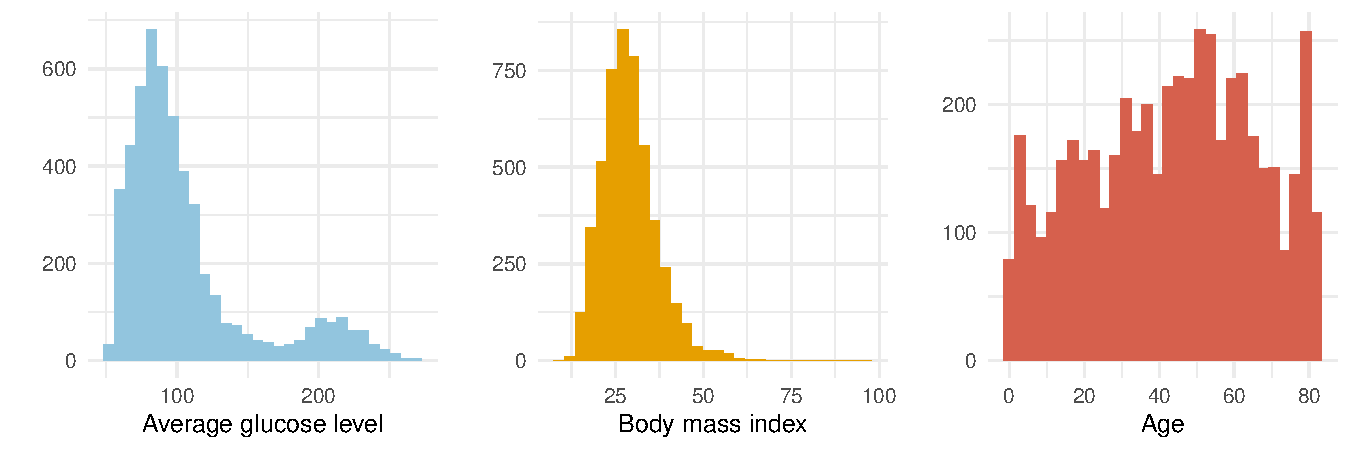
\includegraphics{Build-deploy-stroke-prediction-model-R_files/figure-latex/hist-plots-1.pdf}

The distribution of average glucose level among individuals who
experienced a stroke is visibly multimodal, with a secondary peak above
200. The median average glucose level among stroke cases is around 105.
\textbf{While individuals with average glucose levels above
\textasciitilde{} 200mg/dL constitute a small portion of observations,
they account for approximately 25\% of all stroke cases,} as the
following plot shows.

\begin{Shaded}
\begin{Highlighting}[]
\NormalTok{p1 }\OtherTok{\textless{}{-}} \FunctionTok{ggplot}\NormalTok{(dat, }\FunctionTok{aes}\NormalTok{(}\AttributeTok{x =}\NormalTok{ stroke, }\AttributeTok{y =}\NormalTok{ avg\_glucose\_level, }\AttributeTok{color=}\NormalTok{stroke)) }\SpecialCharTok{+} 
      \FunctionTok{geom\_boxplot}\NormalTok{(}\AttributeTok{outlier.shape =} \ConstantTok{NA}\NormalTok{) }\SpecialCharTok{+}
      \FunctionTok{geom\_jitter}\NormalTok{(}\AttributeTok{width =} \FloatTok{0.2}\NormalTok{, }\AttributeTok{alpha =} \FloatTok{0.6}\NormalTok{, }\AttributeTok{size =} \FloatTok{1.5}\NormalTok{)}\SpecialCharTok{+}
      \FunctionTok{scale\_fill\_brewer}\NormalTok{(}\AttributeTok{palette =} \StringTok{"Set3"}\NormalTok{) }\SpecialCharTok{+}
      \FunctionTok{scale\_color\_brewer}\NormalTok{(}\AttributeTok{palette =} \StringTok{"Set2"}\NormalTok{) }\SpecialCharTok{+}
      \FunctionTok{labs}\NormalTok{(}\AttributeTok{x =} \StringTok{"Stroke"}\NormalTok{, }\AttributeTok{y =} \StringTok{"Average glucose level"}\NormalTok{, }\AttributeTok{color =} \StringTok{"Stroke"}\NormalTok{) }\SpecialCharTok{+}
      \FunctionTok{theme\_minimal}\NormalTok{(}\AttributeTok{base\_size =} \DecValTok{14}\NormalTok{) }\SpecialCharTok{+}
      \FunctionTok{theme}\NormalTok{(}\AttributeTok{legend.position =} \StringTok{"none"}\NormalTok{)  }


\NormalTok{agl\_means }\OtherTok{\textless{}{-}}\NormalTok{ dat }\SpecialCharTok{\%\textgreater{}\%} \FunctionTok{group\_by}\NormalTok{(stroke) }\SpecialCharTok{\%\textgreater{}\%} \FunctionTok{summarise}\NormalTok{(}\AttributeTok{agl\_mean =} \FunctionTok{median}\NormalTok{(avg\_glucose\_level)) }

\NormalTok{p2 }\OtherTok{\textless{}{-}} \FunctionTok{ggplot}\NormalTok{(dat, }\FunctionTok{aes}\NormalTok{(}\AttributeTok{x=}\NormalTok{avg\_glucose\_level, }\AttributeTok{fill=}\NormalTok{stroke)) }\SpecialCharTok{+}  \FunctionTok{geom\_density}\NormalTok{(}\AttributeTok{alpha=}\FloatTok{0.4}\NormalTok{) }\SpecialCharTok{+}
      \FunctionTok{geom\_vline}\NormalTok{(}\AttributeTok{data =}\NormalTok{ agl\_means, }\FunctionTok{aes}\NormalTok{(}\AttributeTok{xintercept=}\NormalTok{agl\_mean, }\AttributeTok{color=}\NormalTok{stroke), }\AttributeTok{linetype=}\StringTok{"dashed"}\NormalTok{)}\SpecialCharTok{+}
      \FunctionTok{labs}\NormalTok{(}\AttributeTok{x =} \StringTok{"Average glucose level"}\NormalTok{, }\AttributeTok{y =} \StringTok{"Density"}\NormalTok{, }\AttributeTok{color =} \StringTok{"stroke"}\NormalTok{) }\SpecialCharTok{+}
      \FunctionTok{scale\_fill\_brewer}\NormalTok{(}\AttributeTok{palette =} \StringTok{"Set3"}\NormalTok{) }\SpecialCharTok{+}
      \FunctionTok{scale\_color\_brewer}\NormalTok{(}\AttributeTok{palette =} \StringTok{"Set2"}\NormalTok{) }\SpecialCharTok{+}
      \FunctionTok{theme\_minimal}\NormalTok{(}\AttributeTok{base\_size =} \DecValTok{14}\NormalTok{) }
      \CommentTok{\#+}
      \CommentTok{\#theme(legend.position = "none")}


\FunctionTok{grid.arrange}\NormalTok{(p1, p2, }\AttributeTok{ncol=}\DecValTok{2}\NormalTok{)}
\end{Highlighting}
\end{Shaded}

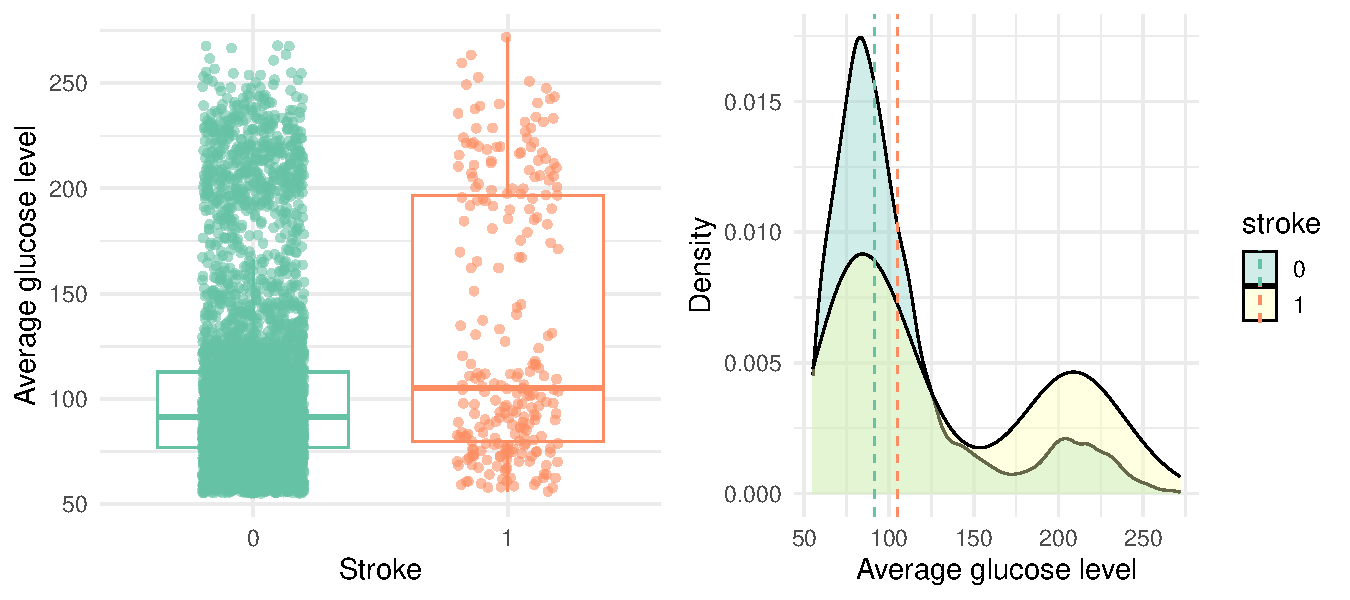
\includegraphics{Build-deploy-stroke-prediction-model-R_files/figure-latex/glucose-stroke-hist-1.pdf}
The distribution of body mass index of stroke individuals is
concentrated around the mean \textasciitilde27. \textbf{For BMI variable
there is much overlap between the stroke and non-stroke cases.}

\begin{Shaded}
\begin{Highlighting}[]
\NormalTok{p1 }\OtherTok{\textless{}{-}} \FunctionTok{ggplot}\NormalTok{(dat, }\FunctionTok{aes}\NormalTok{(}\AttributeTok{x =}\NormalTok{ stroke, }\AttributeTok{y =}\NormalTok{ bmi, }\AttributeTok{color=}\NormalTok{stroke)) }\SpecialCharTok{+} 
      \FunctionTok{geom\_boxplot}\NormalTok{(}\AttributeTok{outlier.shape =} \ConstantTok{NA}\NormalTok{) }\SpecialCharTok{+}
      \FunctionTok{geom\_jitter}\NormalTok{(}\AttributeTok{width =} \FloatTok{0.2}\NormalTok{, }\AttributeTok{alpha =} \FloatTok{0.6}\NormalTok{, }\AttributeTok{size =} \FloatTok{1.5}\NormalTok{)}\SpecialCharTok{+}
      \FunctionTok{scale\_fill\_brewer}\NormalTok{(}\AttributeTok{palette =} \StringTok{"Set3"}\NormalTok{) }\SpecialCharTok{+}
      \FunctionTok{scale\_color\_brewer}\NormalTok{(}\AttributeTok{palette =} \StringTok{"Set2"}\NormalTok{) }\SpecialCharTok{+}
      \FunctionTok{labs}\NormalTok{(}\AttributeTok{x =} \StringTok{"Stroke"}\NormalTok{, }\AttributeTok{y =} \StringTok{"Body mass index"}\NormalTok{, }\AttributeTok{color =} \StringTok{"Stroke"}\NormalTok{) }\SpecialCharTok{+}
      \FunctionTok{theme\_minimal}\NormalTok{(}\AttributeTok{base\_size =} \DecValTok{14}\NormalTok{) }\SpecialCharTok{+}
      \FunctionTok{theme}\NormalTok{(}\AttributeTok{legend.position =} \StringTok{"none"}\NormalTok{)  }


\NormalTok{bmi\_means }\OtherTok{\textless{}{-}}\NormalTok{ dat }\SpecialCharTok{\%\textgreater{}\%} \FunctionTok{filter}\NormalTok{(}\SpecialCharTok{!}\FunctionTok{is.na}\NormalTok{(dat}\SpecialCharTok{$}\NormalTok{bmi)) }\SpecialCharTok{\%\textgreater{}\%}  \FunctionTok{group\_by}\NormalTok{(stroke) }\SpecialCharTok{\%\textgreater{}\%} \FunctionTok{summarise}\NormalTok{(}\AttributeTok{bmi\_mean =} \FunctionTok{mean}\NormalTok{(bmi)) }

\NormalTok{p2 }\OtherTok{\textless{}{-}} \FunctionTok{ggplot}\NormalTok{(dat, }\FunctionTok{aes}\NormalTok{(}\AttributeTok{x=}\NormalTok{bmi, }\AttributeTok{fill=}\NormalTok{stroke)) }\SpecialCharTok{+}  \FunctionTok{geom\_density}\NormalTok{(}\AttributeTok{alpha=}\FloatTok{0.4}\NormalTok{)}\SpecialCharTok{+}
      \FunctionTok{geom\_vline}\NormalTok{(}\AttributeTok{data =}\NormalTok{ bmi\_means, }\FunctionTok{aes}\NormalTok{(}\AttributeTok{xintercept=}\NormalTok{bmi\_mean, }\AttributeTok{color=}\NormalTok{stroke), }\AttributeTok{linetype=}\StringTok{"dashed"}\NormalTok{)}\SpecialCharTok{+}
      \FunctionTok{labs}\NormalTok{(}\AttributeTok{x =} \StringTok{"Body mass index"}\NormalTok{, }\AttributeTok{y =} \StringTok{"Density"}\NormalTok{, }\AttributeTok{color=}\StringTok{"stroke"}\NormalTok{) }\SpecialCharTok{+}
      \FunctionTok{scale\_fill\_brewer}\NormalTok{(}\AttributeTok{palette =} \StringTok{"Set3"}\NormalTok{) }\SpecialCharTok{+}
      \FunctionTok{scale\_color\_brewer}\NormalTok{(}\AttributeTok{palette =} \StringTok{"Set2"}\NormalTok{) }\SpecialCharTok{+}
      \FunctionTok{theme\_minimal}\NormalTok{(}\AttributeTok{base\_size =} \DecValTok{14}\NormalTok{)}

\FunctionTok{grid.arrange}\NormalTok{(p1, p2, }\AttributeTok{ncol=}\DecValTok{2}\NormalTok{)}
\end{Highlighting}
\end{Shaded}

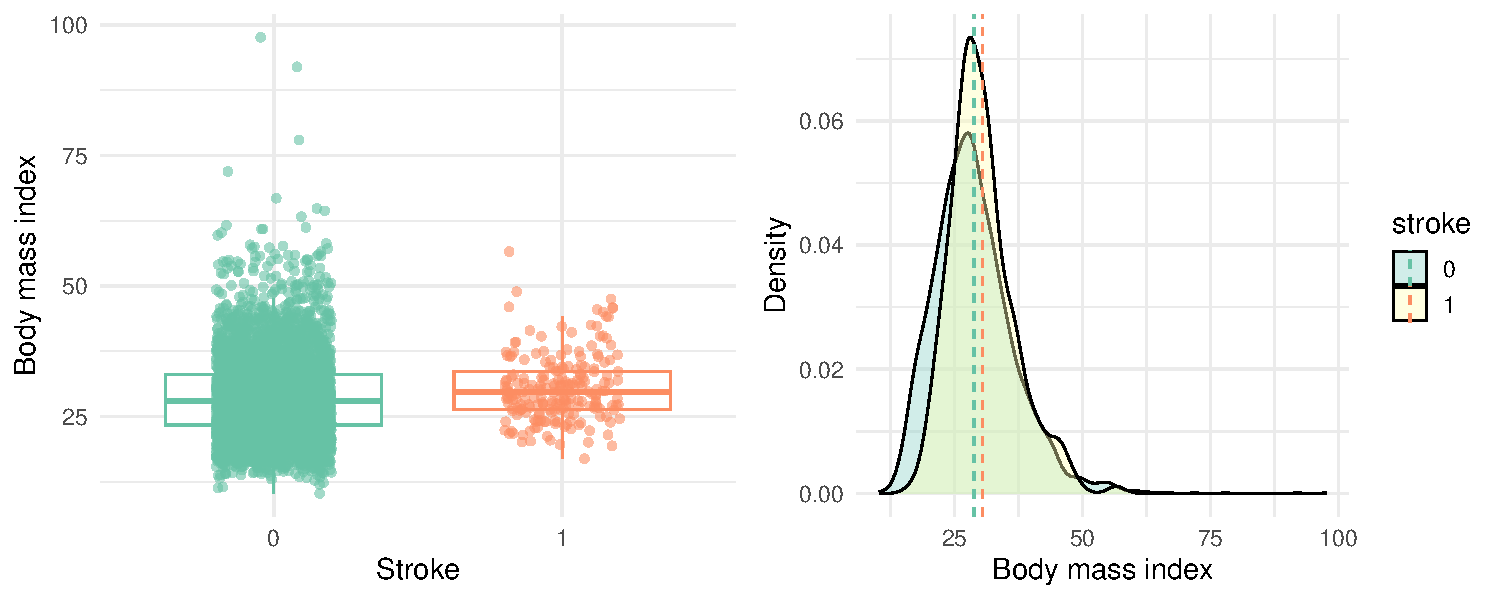
\includegraphics{Build-deploy-stroke-prediction-model-R_files/figure-latex/bmi-stroke-hist-1.pdf}

The following plots show that the age is clearly a risk factor for
stroke: \textbf{75\% of individuals with stroke are aged above
\textasciitilde60}, whereas \textbf{75\% of individuals with no stroke
are aged below \textasciitilde60. For stroke individuals, the
distribution is left skewed with half of strokes happening above the age
70.} There are no stroke cases between the ages 20 and 30 in the data,
but there are 2 children with stroke. The cases involving children can
be considered special cases.

\begin{Shaded}
\begin{Highlighting}[]
\NormalTok{p1 }\OtherTok{\textless{}{-}} \FunctionTok{ggplot}\NormalTok{(dat, }\FunctionTok{aes}\NormalTok{(}\AttributeTok{x =}\NormalTok{ stroke, }\AttributeTok{y =}\NormalTok{ age, }\AttributeTok{color=}\NormalTok{stroke)) }\SpecialCharTok{+} 
      \FunctionTok{geom\_boxplot}\NormalTok{(}\AttributeTok{outlier.shape =} \ConstantTok{NA}\NormalTok{) }\SpecialCharTok{+}
      \FunctionTok{geom\_jitter}\NormalTok{(}\AttributeTok{width =} \FloatTok{0.2}\NormalTok{, }\AttributeTok{alpha =} \FloatTok{0.6}\NormalTok{, }\AttributeTok{size =} \FloatTok{1.5}\NormalTok{)}\SpecialCharTok{+}
      \FunctionTok{scale\_fill\_brewer}\NormalTok{(}\AttributeTok{palette =} \StringTok{"Set3"}\NormalTok{) }\SpecialCharTok{+}
      \FunctionTok{scale\_color\_brewer}\NormalTok{(}\AttributeTok{palette =} \StringTok{"Set2"}\NormalTok{) }\SpecialCharTok{+}
      \FunctionTok{labs}\NormalTok{(}\AttributeTok{x =} \StringTok{"Stroke"}\NormalTok{, }\AttributeTok{y =} \StringTok{"Age"}\NormalTok{, }\AttributeTok{color =} \StringTok{"Stroke"}\NormalTok{) }\SpecialCharTok{+}
      \FunctionTok{theme\_minimal}\NormalTok{(}\AttributeTok{base\_size =} \DecValTok{14}\NormalTok{) }\SpecialCharTok{+}
      \FunctionTok{theme}\NormalTok{(}\AttributeTok{legend.position =} \StringTok{"none"}\NormalTok{)  }


\NormalTok{age\_means }\OtherTok{\textless{}{-}}\NormalTok{ dat }\SpecialCharTok{\%\textgreater{}\%} \FunctionTok{group\_by}\NormalTok{(stroke) }\SpecialCharTok{\%\textgreater{}\%} \FunctionTok{summarise}\NormalTok{(}\AttributeTok{age\_mean =} \FunctionTok{mean}\NormalTok{(age)) }

\NormalTok{p2 }\OtherTok{\textless{}{-}} \FunctionTok{ggplot}\NormalTok{(dat, }\FunctionTok{aes}\NormalTok{(}\AttributeTok{x=}\NormalTok{age, }\AttributeTok{fill=}\NormalTok{stroke)) }\SpecialCharTok{+}  \FunctionTok{geom\_density}\NormalTok{(}\AttributeTok{alpha=}\FloatTok{0.4}\NormalTok{)}\SpecialCharTok{+}
      \FunctionTok{geom\_vline}\NormalTok{(}\AttributeTok{data =}\NormalTok{ age\_means, }\FunctionTok{aes}\NormalTok{(}\AttributeTok{xintercept=}\NormalTok{age\_mean, }\AttributeTok{color=}\NormalTok{stroke), }\AttributeTok{linetype=}\StringTok{"dashed"}\NormalTok{)}\SpecialCharTok{+}
      \FunctionTok{labs}\NormalTok{(}\AttributeTok{x =} \StringTok{"Age"}\NormalTok{, }\AttributeTok{y =} \StringTok{"Density"}\NormalTok{, }\AttributeTok{color =} \StringTok{"Stroke"}\NormalTok{) }\SpecialCharTok{+}
      \FunctionTok{scale\_fill\_brewer}\NormalTok{(}\AttributeTok{palette =} \StringTok{"Set3"}\NormalTok{) }\SpecialCharTok{+}
      \FunctionTok{scale\_color\_brewer}\NormalTok{(}\AttributeTok{palette =} \StringTok{"Set2"}\NormalTok{) }\SpecialCharTok{+}
      \FunctionTok{theme\_minimal}\NormalTok{(}\AttributeTok{base\_size =} \DecValTok{14}\NormalTok{) }\SpecialCharTok{+}
      \FunctionTok{theme}\NormalTok{(}\AttributeTok{legend.position =} \StringTok{"none"}\NormalTok{)}

\FunctionTok{grid.arrange}\NormalTok{(p1, p2, }\AttributeTok{ncol=}\DecValTok{2}\NormalTok{)}
\end{Highlighting}
\end{Shaded}

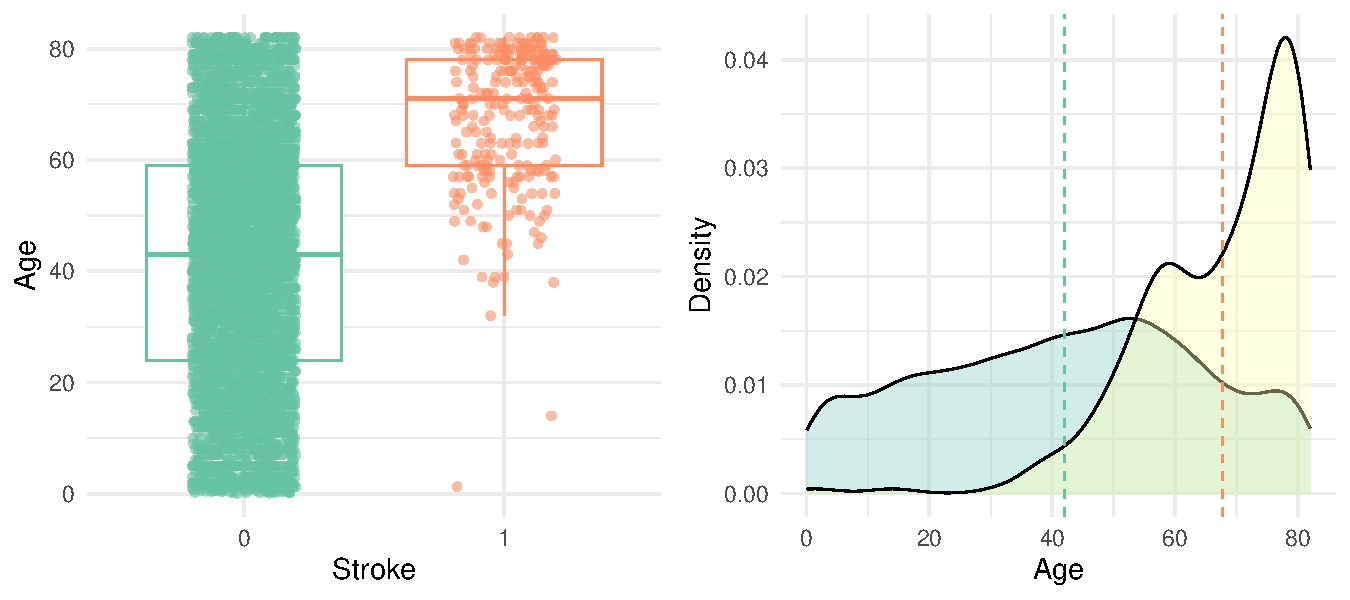
\includegraphics{Build-deploy-stroke-prediction-model-R_files/figure-latex/age-stroke-plot-1.pdf}

The relationship between average glucose level and heart disease.

\begin{Shaded}
\begin{Highlighting}[]
\NormalTok{p1 }\OtherTok{\textless{}{-}} \FunctionTok{ggplot}\NormalTok{(dat, }\FunctionTok{aes}\NormalTok{(}\AttributeTok{x =}\NormalTok{ heart\_disease, }\AttributeTok{y =}\NormalTok{ avg\_glucose\_level, }\AttributeTok{color=}\NormalTok{heart\_disease)) }\SpecialCharTok{+} 
      \FunctionTok{geom\_boxplot}\NormalTok{(}\AttributeTok{outlier.shape =} \ConstantTok{NA}\NormalTok{) }\SpecialCharTok{+}
      \FunctionTok{geom\_jitter}\NormalTok{(}\AttributeTok{width =} \FloatTok{0.2}\NormalTok{, }\AttributeTok{alpha =} \FloatTok{0.6}\NormalTok{, }\AttributeTok{size =} \FloatTok{1.5}\NormalTok{)}\SpecialCharTok{+}
      \FunctionTok{scale\_fill\_brewer}\NormalTok{(}\AttributeTok{palette =} \StringTok{"Set3"}\NormalTok{) }\SpecialCharTok{+}
      \FunctionTok{scale\_color\_brewer}\NormalTok{(}\AttributeTok{palette =} \StringTok{"Set2"}\NormalTok{) }\SpecialCharTok{+}
      \FunctionTok{labs}\NormalTok{(}\AttributeTok{x =} \StringTok{"Heart disease"}\NormalTok{, }\AttributeTok{y =} \StringTok{"Average glucose level"}\NormalTok{, }\AttributeTok{color =} \StringTok{"heart\_disease"}\NormalTok{) }\SpecialCharTok{+}
      \FunctionTok{theme\_minimal}\NormalTok{(}\AttributeTok{base\_size =} \DecValTok{14}\NormalTok{) }\SpecialCharTok{+}
      \FunctionTok{theme}\NormalTok{(}\AttributeTok{legend.position =} \StringTok{"none"}\NormalTok{)  }


\NormalTok{agl\_means }\OtherTok{\textless{}{-}}\NormalTok{ dat }\SpecialCharTok{\%\textgreater{}\%} \FunctionTok{group\_by}\NormalTok{(heart\_disease) }\SpecialCharTok{\%\textgreater{}\%} \FunctionTok{summarise}\NormalTok{(}\AttributeTok{agl\_mean =} \FunctionTok{median}\NormalTok{(avg\_glucose\_level)) }

\NormalTok{p2 }\OtherTok{\textless{}{-}} \FunctionTok{ggplot}\NormalTok{(dat, }\FunctionTok{aes}\NormalTok{(}\AttributeTok{x=}\NormalTok{avg\_glucose\_level, }\AttributeTok{fill=}\NormalTok{heart\_disease)) }\SpecialCharTok{+}  \FunctionTok{geom\_density}\NormalTok{(}\AttributeTok{alpha=}\FloatTok{0.4}\NormalTok{) }\SpecialCharTok{+}
      \FunctionTok{geom\_vline}\NormalTok{(}\AttributeTok{data =}\NormalTok{ agl\_means, }\FunctionTok{aes}\NormalTok{(}\AttributeTok{xintercept=}\NormalTok{agl\_mean, }\AttributeTok{color=}\NormalTok{heart\_disease), }\AttributeTok{linetype=}\StringTok{"dashed"}\NormalTok{)}\SpecialCharTok{+}
      \FunctionTok{labs}\NormalTok{(}\AttributeTok{x =} \StringTok{"Average glucose level"}\NormalTok{, }\AttributeTok{y =} \StringTok{"Density"}\NormalTok{, }\AttributeTok{color =} \StringTok{"heart\_disease"}\NormalTok{) }\SpecialCharTok{+}
      \FunctionTok{scale\_fill\_brewer}\NormalTok{(}\AttributeTok{palette =} \StringTok{"Set3"}\NormalTok{) }\SpecialCharTok{+}
      \FunctionTok{scale\_color\_brewer}\NormalTok{(}\AttributeTok{palette =} \StringTok{"Set2"}\NormalTok{) }\SpecialCharTok{+}
      \FunctionTok{theme\_minimal}\NormalTok{(}\AttributeTok{base\_size =} \DecValTok{14}\NormalTok{) }

\FunctionTok{grid.arrange}\NormalTok{(p1, p2, }\AttributeTok{ncol=}\DecValTok{2}\NormalTok{)}
\end{Highlighting}
\end{Shaded}

\includegraphics{Build-deploy-stroke-prediction-model-R_files/figure-latex/glucose-heart_disease-hist-1.pdf}

Next, we analyze pairwise relationships between these variables.
\textbf{For stroke individuals, there is a negative correlation between
the age and the body mass index. This association is positive for
non-stroke cases.} The association between the average glucose level and
body mass index is higher than it is in the non-stroke case.

\begin{Shaded}
\begin{Highlighting}[]
\FunctionTok{ggpairs}\NormalTok{(dat, }\AttributeTok{columns=}\FunctionTok{c}\NormalTok{(}\DecValTok{2}\NormalTok{, }\DecValTok{8}\NormalTok{, }\DecValTok{9}\NormalTok{), }\FunctionTok{aes}\NormalTok{(}\AttributeTok{color=}\NormalTok{stroke, }\AttributeTok{alpha=}\FloatTok{0.3}\NormalTok{),}
        \AttributeTok{lower=}\FunctionTok{list}\NormalTok{(}\AttributeTok{continuous=}\StringTok{"smooth"}\NormalTok{), }\AttributeTok{diag=}\FunctionTok{list}\NormalTok{(}\AttributeTok{continuous=}\StringTok{"densityDiag"}\NormalTok{))}\SpecialCharTok{+}
  \FunctionTok{scale\_fill\_brewer}\NormalTok{(}\AttributeTok{palette =} \StringTok{"Set3"}\NormalTok{) }\SpecialCharTok{+}
  \FunctionTok{scale\_color\_brewer}\NormalTok{(}\AttributeTok{palette =} \StringTok{"Set2"}\NormalTok{)}
\end{Highlighting}
\end{Shaded}

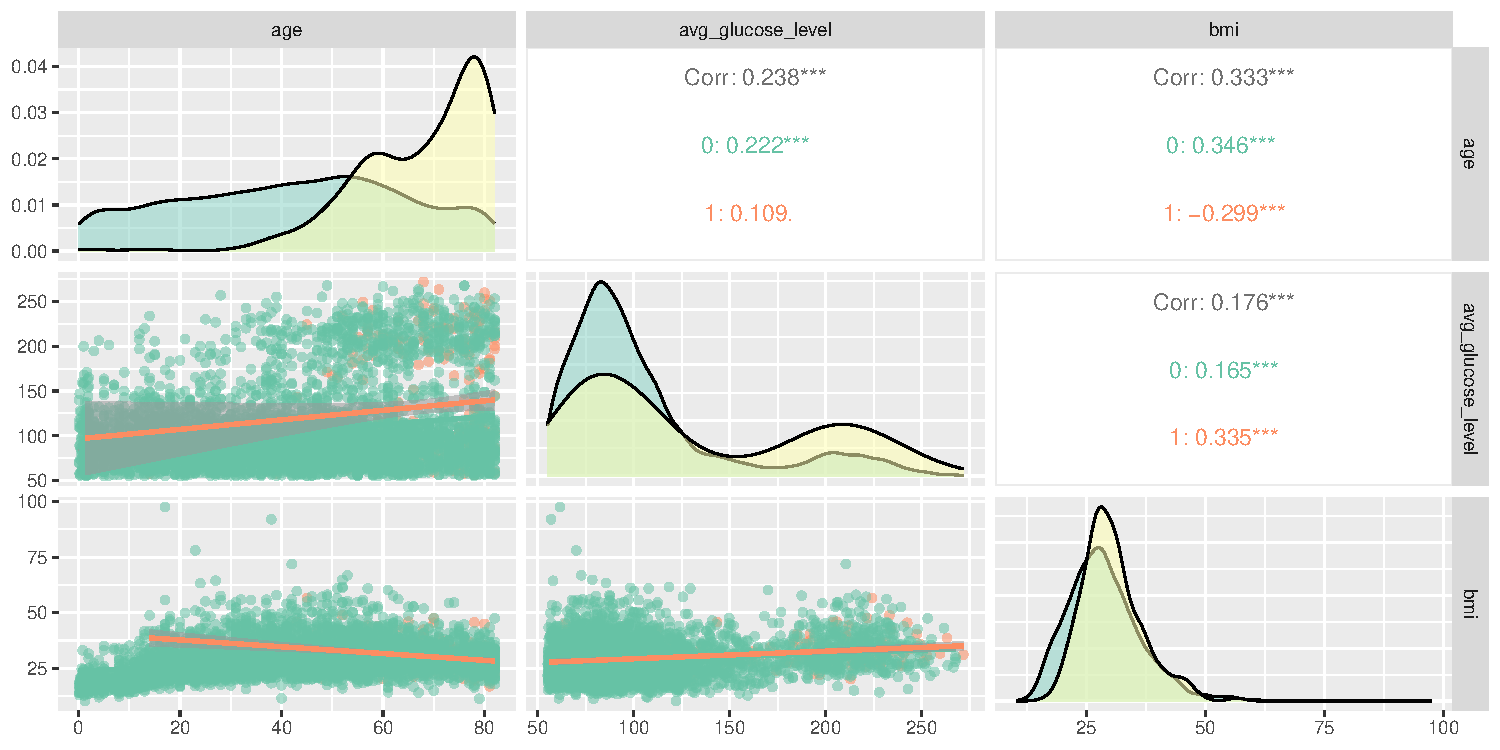
\includegraphics{Build-deploy-stroke-prediction-model-R_files/figure-latex/pairwise-plot-1.pdf}

\textbf{75\%} of the hypertension individuals are above the age of
\textbf{\textasciitilde52} and \textbf{half} of the hypertension
individuals are above the age of \textbf{\textasciitilde62}.
\textbf{Stroke appears later in life, regardless of hypertension,
however the hypertension individuals who experienced stroke are
generally older individuals}.

\begin{Shaded}
\begin{Highlighting}[]
\NormalTok{p1 }\OtherTok{\textless{}{-}} \FunctionTok{ggplot}\NormalTok{(dat, }\FunctionTok{aes}\NormalTok{(}\AttributeTok{x =}\NormalTok{ hypertension, }\AttributeTok{y =}\NormalTok{ age, }\AttributeTok{fill =}\NormalTok{ hypertension)) }\SpecialCharTok{+} 
      \FunctionTok{geom\_boxplot}\NormalTok{(}\AttributeTok{outlier.shape =} \ConstantTok{NA}\NormalTok{, }\AttributeTok{position =} \FunctionTok{position\_dodge}\NormalTok{(}\FloatTok{0.8}\NormalTok{)) }\SpecialCharTok{+}
      \FunctionTok{geom\_jitter}\NormalTok{(}\FunctionTok{aes}\NormalTok{(}\AttributeTok{color=}\NormalTok{hypertension), }\AttributeTok{width=}\FloatTok{0.2}\NormalTok{, }\AttributeTok{alpha =} \FloatTok{0.5}\NormalTok{, }\AttributeTok{size =} \FloatTok{1.2}\NormalTok{) }\SpecialCharTok{+}
      \FunctionTok{scale\_fill\_brewer}\NormalTok{(}\AttributeTok{palette =} \StringTok{"Set2"}\NormalTok{) }\SpecialCharTok{+}
      \FunctionTok{scale\_color\_brewer}\NormalTok{(}\AttributeTok{palette =} \StringTok{"Set2"}\NormalTok{) }\SpecialCharTok{+}
      \FunctionTok{labs}\NormalTok{(}\AttributeTok{x =} \StringTok{"Hypertension"}\NormalTok{, }\AttributeTok{y =} \StringTok{"Age"}\NormalTok{, }\AttributeTok{title =} \StringTok{"Age distribution by hypertension"}\NormalTok{) }\SpecialCharTok{+}
      \FunctionTok{theme\_minimal}\NormalTok{(}\AttributeTok{base\_size =} \DecValTok{14}\NormalTok{)}\SpecialCharTok{+}
      \FunctionTok{theme}\NormalTok{(}\AttributeTok{plot.title =} \FunctionTok{element\_text}\NormalTok{(}\AttributeTok{hjust =} \FloatTok{0.5}\NormalTok{, }\AttributeTok{size =} \DecValTok{16}\NormalTok{))}


\NormalTok{p2 }\OtherTok{\textless{}{-}} \FunctionTok{ggplot}\NormalTok{(dat, }\FunctionTok{aes}\NormalTok{(}\AttributeTok{x =}\NormalTok{ hypertension, }\AttributeTok{y =}\NormalTok{ age, }\AttributeTok{fill =}\NormalTok{ stroke)) }\SpecialCharTok{+} 
      \FunctionTok{geom\_boxplot}\NormalTok{(}\AttributeTok{outlier.shape =} \ConstantTok{NA}\NormalTok{, }\AttributeTok{position =} \FunctionTok{position\_dodge}\NormalTok{(}\FloatTok{0.8}\NormalTok{)) }\SpecialCharTok{+}
      \FunctionTok{geom\_jitter}\NormalTok{(}\FunctionTok{aes}\NormalTok{(}\AttributeTok{color =}\NormalTok{ stroke), }
                  \AttributeTok{position =} \FunctionTok{position\_jitterdodge}\NormalTok{(}\AttributeTok{jitter.width =} \FloatTok{0.2}\NormalTok{, }\AttributeTok{dodge.width =} \FloatTok{0.8}\NormalTok{),}
                  \AttributeTok{alpha =} \FloatTok{0.5}\NormalTok{, }\AttributeTok{size =} \FloatTok{1.2}\NormalTok{) }\SpecialCharTok{+}
      \FunctionTok{scale\_fill\_brewer}\NormalTok{(}\AttributeTok{palette =} \StringTok{"Set3"}\NormalTok{) }\SpecialCharTok{+}
      \FunctionTok{scale\_color\_brewer}\NormalTok{(}\AttributeTok{palette =} \StringTok{"Set2"}\NormalTok{) }\SpecialCharTok{+}
      \FunctionTok{labs}\NormalTok{(}\AttributeTok{x =} \StringTok{"Hypertension"}\NormalTok{, }\AttributeTok{y =} \StringTok{"Age"}\NormalTok{, }\AttributeTok{fill =} \StringTok{"Stroke"}\NormalTok{, }\AttributeTok{color =} \StringTok{"Stroke"}\NormalTok{, }
           \AttributeTok{title =} \StringTok{"Age distribution by hypertension and stroke"}\NormalTok{) }\SpecialCharTok{+}
      \FunctionTok{theme\_minimal}\NormalTok{(}\AttributeTok{base\_size =} \DecValTok{14}\NormalTok{)}\SpecialCharTok{+}
      \FunctionTok{theme}\NormalTok{(}\AttributeTok{plot.title =} \FunctionTok{element\_text}\NormalTok{(}\AttributeTok{hjust =} \FloatTok{0.5}\NormalTok{, }\AttributeTok{size =} \DecValTok{16}\NormalTok{))}

\FunctionTok{grid.arrange}\NormalTok{(p1, p2, }\AttributeTok{ncol=}\DecValTok{2}\NormalTok{)}
\end{Highlighting}
\end{Shaded}

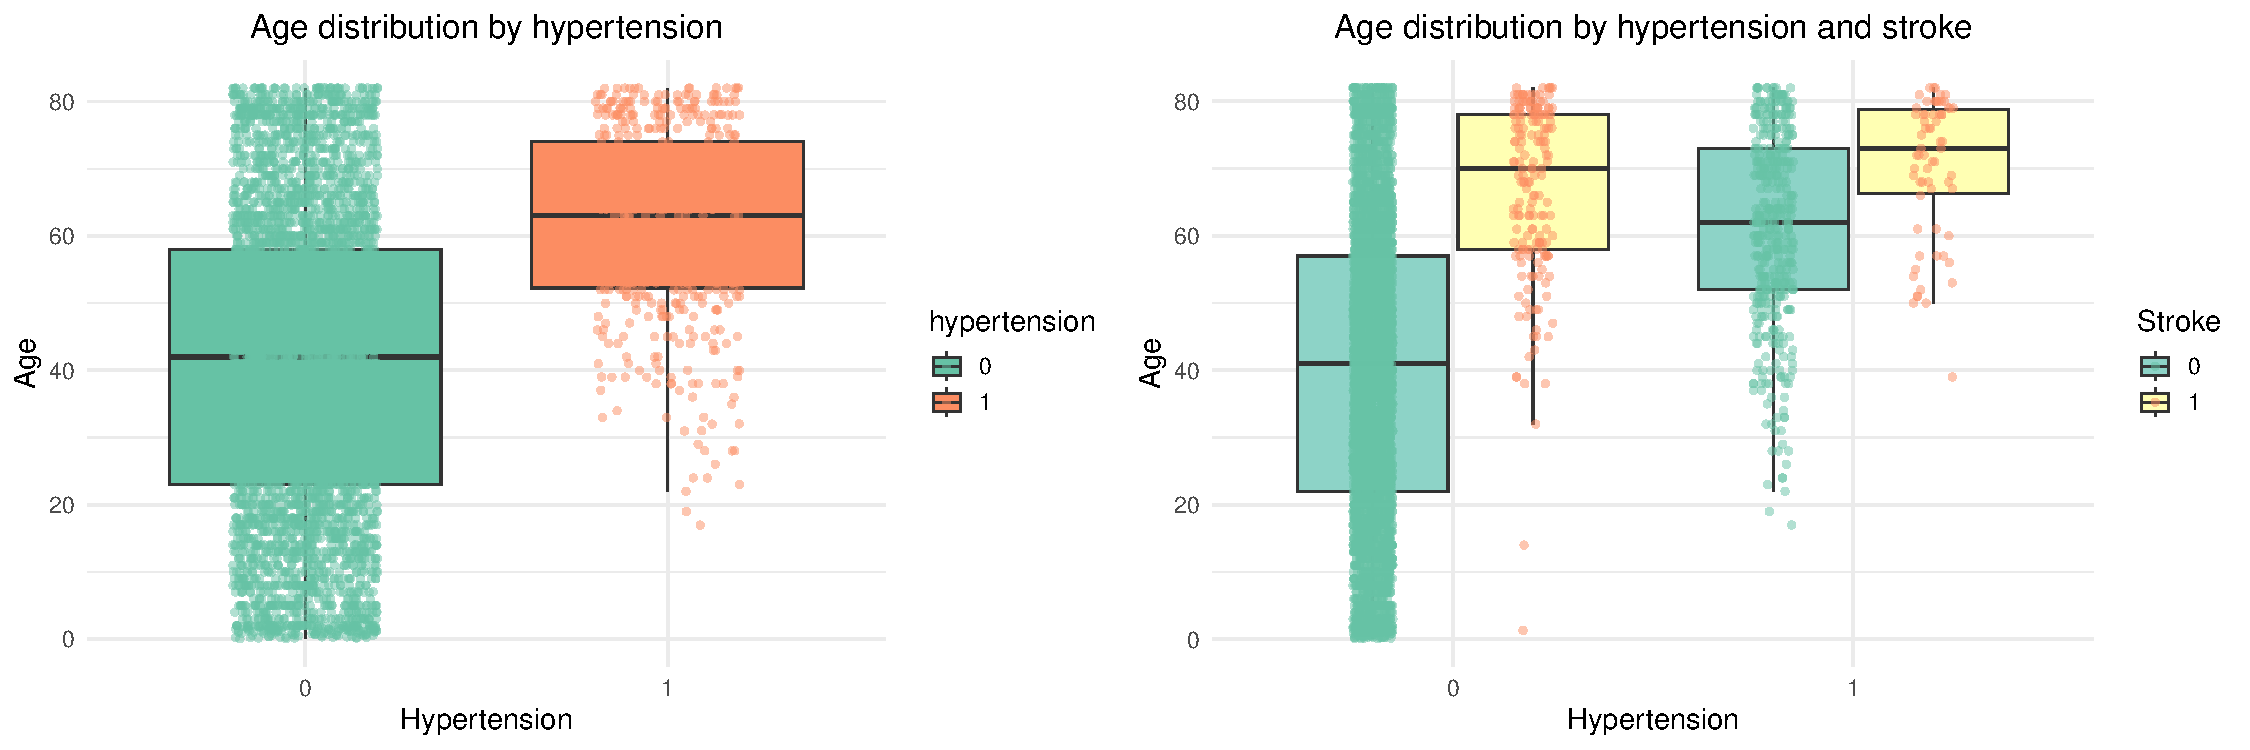
\includegraphics{Build-deploy-stroke-prediction-model-R_files/figure-latex/pairwise_age_hypertension-1.pdf}

The median age for heart disease is higher than that for hypertension:
above 70. Similarly, \textbf{stroke appears later in life, regardless of
heart disease, however there is less variability in the age distribution
of individuals with heart disease and stroke: they are predominantly
older.}

\begin{Shaded}
\begin{Highlighting}[]
\NormalTok{p1 }\OtherTok{\textless{}{-}} \FunctionTok{ggplot}\NormalTok{(dat, }\FunctionTok{aes}\NormalTok{(}\AttributeTok{x =}\NormalTok{ heart\_disease, }\AttributeTok{y =}\NormalTok{ age, }\AttributeTok{fill =}\NormalTok{ heart\_disease)) }\SpecialCharTok{+} 
      \FunctionTok{geom\_boxplot}\NormalTok{(}\AttributeTok{outlier.shape =} \ConstantTok{NA}\NormalTok{, }\AttributeTok{position =} \FunctionTok{position\_dodge}\NormalTok{(}\FloatTok{0.8}\NormalTok{)) }\SpecialCharTok{+}
      \FunctionTok{geom\_jitter}\NormalTok{(}\FunctionTok{aes}\NormalTok{(}\AttributeTok{color=}\NormalTok{heart\_disease), }\AttributeTok{width=}\FloatTok{0.2}\NormalTok{, }\AttributeTok{alpha =} \FloatTok{0.5}\NormalTok{, }\AttributeTok{size =} \FloatTok{1.2}\NormalTok{) }\SpecialCharTok{+}
      \FunctionTok{scale\_fill\_brewer}\NormalTok{(}\AttributeTok{palette =} \StringTok{"Set2"}\NormalTok{) }\SpecialCharTok{+}
      \FunctionTok{scale\_color\_brewer}\NormalTok{(}\AttributeTok{palette =} \StringTok{"Set2"}\NormalTok{) }\SpecialCharTok{+}
      \FunctionTok{labs}\NormalTok{(}\AttributeTok{x =} \StringTok{"Heart disease"}\NormalTok{, }\AttributeTok{y =} \StringTok{"Age"}\NormalTok{, }\AttributeTok{title =} \StringTok{"Age distribution by heart disease"}\NormalTok{) }\SpecialCharTok{+}
      \FunctionTok{theme\_minimal}\NormalTok{(}\AttributeTok{base\_size =} \DecValTok{14}\NormalTok{)}\SpecialCharTok{+}
      \FunctionTok{theme}\NormalTok{(}\AttributeTok{plot.title =} \FunctionTok{element\_text}\NormalTok{(}\AttributeTok{hjust =} \FloatTok{0.5}\NormalTok{, }\AttributeTok{size =} \DecValTok{16}\NormalTok{))}


\NormalTok{p2 }\OtherTok{\textless{}{-}} \FunctionTok{ggplot}\NormalTok{(dat, }\FunctionTok{aes}\NormalTok{(}\AttributeTok{x =}\NormalTok{ heart\_disease, }\AttributeTok{y =}\NormalTok{ age, }\AttributeTok{fill =}\NormalTok{ stroke)) }\SpecialCharTok{+} 
      \FunctionTok{geom\_boxplot}\NormalTok{(}\AttributeTok{outlier.shape =} \ConstantTok{NA}\NormalTok{, }\AttributeTok{position =} \FunctionTok{position\_dodge}\NormalTok{(}\FloatTok{0.8}\NormalTok{)) }\SpecialCharTok{+}
      \FunctionTok{geom\_jitter}\NormalTok{(}\FunctionTok{aes}\NormalTok{(}\AttributeTok{color =}\NormalTok{ stroke), }
                  \AttributeTok{position =} \FunctionTok{position\_jitterdodge}\NormalTok{(}\AttributeTok{jitter.width =} \FloatTok{0.2}\NormalTok{, }\AttributeTok{dodge.width =} \FloatTok{0.8}\NormalTok{),}
                  \AttributeTok{alpha =} \FloatTok{0.5}\NormalTok{, }\AttributeTok{size =} \FloatTok{1.2}\NormalTok{) }\SpecialCharTok{+}
      \FunctionTok{scale\_fill\_brewer}\NormalTok{(}\AttributeTok{palette =} \StringTok{"Set3"}\NormalTok{) }\SpecialCharTok{+}
      \FunctionTok{scale\_color\_brewer}\NormalTok{(}\AttributeTok{palette =} \StringTok{"Set2"}\NormalTok{) }\SpecialCharTok{+}
      \FunctionTok{labs}\NormalTok{(}
        \AttributeTok{x =} \StringTok{"Heart disease"}\NormalTok{,}
        \AttributeTok{y =} \StringTok{"Age"}\NormalTok{,}
        \AttributeTok{fill =} \StringTok{"Stroke"}\NormalTok{,}
        \AttributeTok{color =} \StringTok{"Stroke"}\NormalTok{,}
        \AttributeTok{title =} \StringTok{"Age distribution by heart disease and stroke"}
\NormalTok{      ) }\SpecialCharTok{+}
      \FunctionTok{theme\_minimal}\NormalTok{(}\AttributeTok{base\_size =} \DecValTok{14}\NormalTok{)}\SpecialCharTok{+}
      \FunctionTok{theme}\NormalTok{(}
         \AttributeTok{plot.title =} \FunctionTok{element\_text}\NormalTok{(}\AttributeTok{hjust =} \FloatTok{0.5}\NormalTok{, }\AttributeTok{size =} \DecValTok{16}\NormalTok{)}
\NormalTok{      )}

\FunctionTok{grid.arrange}\NormalTok{(p1, p2, }\AttributeTok{ncol=}\DecValTok{2}\NormalTok{)}
\end{Highlighting}
\end{Shaded}

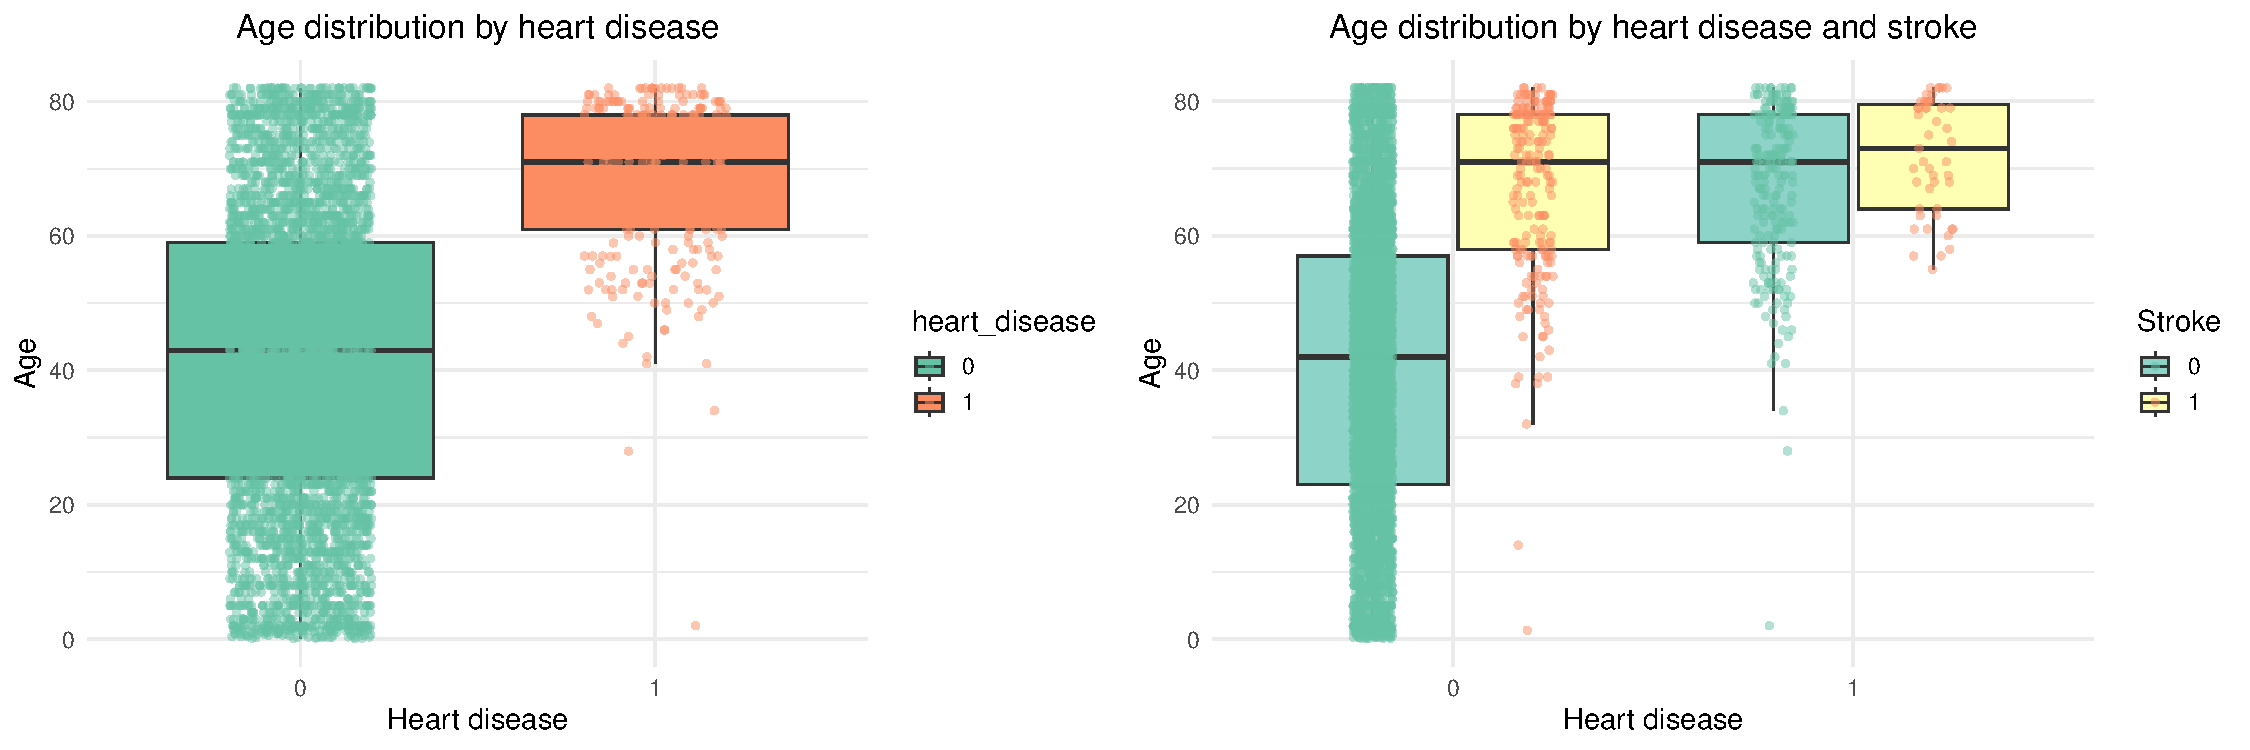
\includegraphics{Build-deploy-stroke-prediction-model-R_files/figure-latex/pairwise_age_heart_disease-1.pdf}

The following plot shows the age distribution across combinations of
hypertension and heart diseases. For instance 1\_1 indicates the
individuals who had both hypertension and heart disease. We separate the
boxplots by stroke condition.

\begin{Shaded}
\begin{Highlighting}[]
\NormalTok{stroke\_hypert\_heartd }\OtherTok{\textless{}{-}}\NormalTok{ dat }\SpecialCharTok{\%\textgreater{}\%}\FunctionTok{mutate}\NormalTok{(}\AttributeTok{hyp\_hd =} \FunctionTok{interaction}\NormalTok{(hypertension, heart\_disease, }\AttributeTok{sep =} \StringTok{"\_"}\NormalTok{))}

\FunctionTok{ggplot}\NormalTok{(stroke\_hypert\_heartd, }\FunctionTok{aes}\NormalTok{(}\AttributeTok{x =}\NormalTok{ hyp\_hd, }\AttributeTok{y =}\NormalTok{ age, }\AttributeTok{fill =}\NormalTok{ stroke)) }\SpecialCharTok{+}
    \FunctionTok{geom\_boxplot}\NormalTok{(}\AttributeTok{position =} \FunctionTok{position\_dodge}\NormalTok{(}\AttributeTok{width =} \FloatTok{0.75}\NormalTok{), }\AttributeTok{outlier.shape =} \ConstantTok{NA}\NormalTok{) }\SpecialCharTok{+}
    \FunctionTok{geom\_jitter}\NormalTok{(}\FunctionTok{aes}\NormalTok{(}\AttributeTok{color =}\NormalTok{ stroke),  }
                \AttributeTok{position =} \FunctionTok{position\_jitterdodge}\NormalTok{(}\AttributeTok{jitter.width =} \FloatTok{0.2}\NormalTok{, }\AttributeTok{dodge.width =} \FloatTok{0.75}\NormalTok{),}
                \AttributeTok{alpha =} \FloatTok{0.4}\NormalTok{, }\AttributeTok{size =} \FloatTok{1.2}\NormalTok{) }\SpecialCharTok{+}
    \FunctionTok{scale\_fill\_brewer}\NormalTok{(}\AttributeTok{palette =} \StringTok{"Set3"}\NormalTok{) }\SpecialCharTok{+}
    \FunctionTok{scale\_color\_brewer}\NormalTok{(}\AttributeTok{palette =} \StringTok{"Set2"}\NormalTok{) }\SpecialCharTok{+}
    \FunctionTok{labs}\NormalTok{(}
      \AttributeTok{x =} \StringTok{"Hypertension\_heart disease"}\NormalTok{,}
      \AttributeTok{y =} \StringTok{"Age"}\NormalTok{,}
      \AttributeTok{title =} \StringTok{"Age distribution by hypertension \& heart disease, split by stroke"}
\NormalTok{    ) }\SpecialCharTok{+}
    \FunctionTok{theme\_minimal}\NormalTok{(}\AttributeTok{base\_size =} \DecValTok{14}\NormalTok{) }\SpecialCharTok{+}
    \FunctionTok{theme}\NormalTok{(}\AttributeTok{plot.title =} \FunctionTok{element\_text}\NormalTok{(}\AttributeTok{hjust =} \FloatTok{0.5}\NormalTok{, }\AttributeTok{size =} \DecValTok{16}\NormalTok{))}
\end{Highlighting}
\end{Shaded}

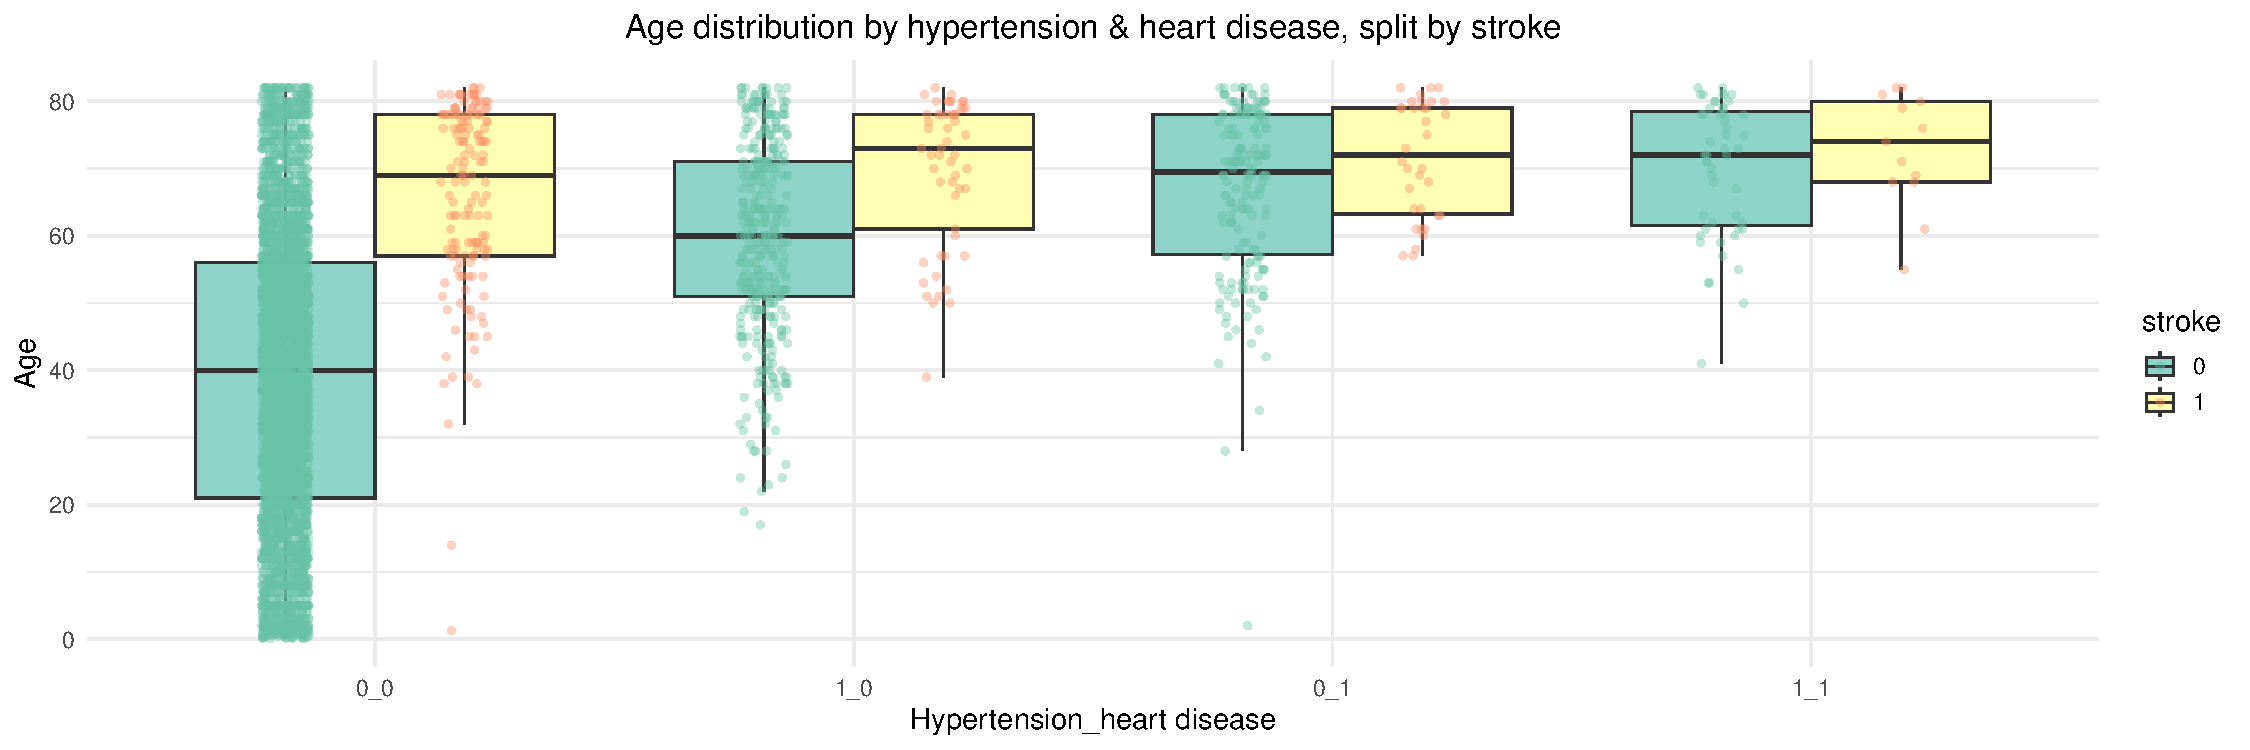
\includegraphics{Build-deploy-stroke-prediction-model-R_files/figure-latex/pairwise_age_heartd_hypert-1.pdf}

\subsubsection{\texorpdfstring{\textbf{Epidemiological
analysis}}{Epidemiological analysis}}\label{epidemiological-analysis}

In this section, we will do some statistical analysis of association
between variables.

\paragraph{\texorpdfstring{\textbf{Odds
ratio}}{Odds ratio}}\label{odds-ratio}

To compute the odds ratio we use \textbf{epitools package}. The outcome
of interest is stroke, and the exposures are: hypertension, heart
disease, average glucose level, and age.

The following odds ratio computation shows that the \textbf{odds of
stroke in hypertensive individuals is \textasciitilde3.7 times higher
than that in non-hypertensive individuals}.

\begin{Shaded}
\begin{Highlighting}[]
\NormalTok{tbl\_hypertension }\OtherTok{\textless{}{-}} \FunctionTok{table}\NormalTok{(dat}\SpecialCharTok{$}\NormalTok{stroke, dat}\SpecialCharTok{$}\NormalTok{hypertension)}

\FunctionTok{oddsratio}\NormalTok{(tbl\_hypertension)}
\end{Highlighting}
\end{Shaded}

\begin{verbatim}
## $data
##        
##            0   1 Total
##   0     4429 432  4861
##   1      183  66   249
##   Total 4612 498  5110
## 
## $measure
##    odds ratio with 95% C.I.
##     estimate    lower    upper
##   0 1.000000       NA       NA
##   1 3.701246 2.729655 4.964923
## 
## $p.value
##    two-sided
##      midp.exact fisher.exact   chi.square
##   0          NA           NA           NA
##   1 5.77316e-15 4.549182e-15 6.068123e-20
## 
## $correction
## [1] FALSE
## 
## attr(,"method")
## [1] "median-unbiased estimate & mid-p exact CI"
\end{verbatim}

Also the \textbf{odds of stroke in individuals with heart disease is
\textasciitilde4.71 times higher than that in individuals with no heart
disease.}

\begin{Shaded}
\begin{Highlighting}[]
\NormalTok{tbl\_heart\_disease }\OtherTok{\textless{}{-}} \FunctionTok{table}\NormalTok{(dat}\SpecialCharTok{$}\NormalTok{stroke, dat}\SpecialCharTok{$}\NormalTok{heart\_disease)}

\FunctionTok{oddsratio}\NormalTok{(tbl\_heart\_disease)}
\end{Highlighting}
\end{Shaded}

\begin{verbatim}
## $data
##        
##            0   1 Total
##   0     4632 229  4861
##   1      202  47   249
##   Total 4834 276  5110
## 
## $measure
##    odds ratio with 95% C.I.
##     estimate    lower    upper
##   0 1.000000       NA       NA
##   1 4.714026 3.309098 6.601552
## 
## $p.value
##    two-sided
##       midp.exact fisher.exact  chi.square
##   0           NA           NA          NA
##   1 8.881784e-15 7.283093e-15 5.20011e-22
## 
## $correction
## [1] FALSE
## 
## attr(,"method")
## [1] "median-unbiased estimate & mid-p exact CI"
\end{verbatim}

To do odds ratio analysis with average glucose level, we bin it into two
groups at the level of 150. \textbf{Individuals with average glucose
level \textgreater150 have \textasciitilde3.7 times higher odds of
stroke than those with glucose ≤150.}

\begin{Shaded}
\begin{Highlighting}[]
\NormalTok{stroke\_agl }\OtherTok{\textless{}{-}}\NormalTok{ dat }\SpecialCharTok{\%\textgreater{}\%} \FunctionTok{mutate}\NormalTok{(}\AttributeTok{agl\_group =} \FunctionTok{cut}\NormalTok{(avg\_glucose\_level, }\AttributeTok{breaks =} \FunctionTok{c}\NormalTok{(}\DecValTok{0}\NormalTok{, }\DecValTok{150}\NormalTok{, }\FunctionTok{max}\NormalTok{(dat}\SpecialCharTok{$}\NormalTok{avg\_glucose\_level)))) }\SpecialCharTok{\%\textgreater{}\%} \FunctionTok{select}\NormalTok{(}\FunctionTok{c}\NormalTok{(stroke, agl\_group))}

\NormalTok{tbl\_agl }\OtherTok{\textless{}{-}} \FunctionTok{table}\NormalTok{(stroke\_agl}\SpecialCharTok{$}\NormalTok{stroke, stroke\_agl}\SpecialCharTok{$}\NormalTok{agl\_group)}

\FunctionTok{oddsratio}\NormalTok{(tbl\_agl)}
\end{Highlighting}
\end{Shaded}

\begin{verbatim}
## $data
##        
##         (0,150] (150,272] Total
##   0        4221       640  4861
##   1         159        90   249
##   Total    4380       730  5110
## 
## $measure
##    odds ratio with 95% C.I.
##     estimate    lower    upper
##   0 1.000000       NA       NA
##   1 3.734437 2.836751 4.889724
## 
## $p.value
##    two-sided
##     midp.exact fisher.exact   chi.square
##   0         NA           NA           NA
##   1          0 6.607959e-19 5.174082e-24
## 
## $correction
## [1] FALSE
## 
## attr(,"method")
## [1] "median-unbiased estimate & mid-p exact CI"
\end{verbatim}

\textbf{Odds of stroke in individuals aged above 60 is
\textasciitilde8.13 times higher than that in indivduals aged less than
60.} Thus we see that \textbf{age is a very important risk factor}. This
result is \textbf{statistically very significant, the confidence
interval does not contain 1}, as the two result reported above.

\begin{Shaded}
\begin{Highlighting}[]
\NormalTok{stroke\_age }\OtherTok{\textless{}{-}}\NormalTok{ dat }\SpecialCharTok{\%\textgreater{}\%} \FunctionTok{mutate}\NormalTok{(}\AttributeTok{age\_group =} \FunctionTok{cut}\NormalTok{(age, }\AttributeTok{breaks =} \FunctionTok{c}\NormalTok{(}\DecValTok{0}\NormalTok{, }\DecValTok{60}\NormalTok{, }\FunctionTok{max}\NormalTok{(dat}\SpecialCharTok{$}\NormalTok{age)), }\AttributeTok{labels=}\FunctionTok{c}\NormalTok{(}\StringTok{"0"}\NormalTok{, }\StringTok{"1"}\NormalTok{))) }\SpecialCharTok{\%\textgreater{}\%} \FunctionTok{select}\NormalTok{(}\FunctionTok{c}\NormalTok{(stroke, age\_group))}

\NormalTok{tbl\_age }\OtherTok{\textless{}{-}} \FunctionTok{table}\NormalTok{(stroke\_age}\SpecialCharTok{$}\NormalTok{stroke, stroke\_age}\SpecialCharTok{$}\NormalTok{age\_group)}

\FunctionTok{oddsratio}\NormalTok{(tbl\_age)}
\end{Highlighting}
\end{Shaded}

\begin{verbatim}
## $data
##        
##            0    1 Total
##   0     3734 1127  4861
##   1       72  177   249
##   Total 3806 1304  5110
## 
## $measure
##    odds ratio with 95% C.I.
##     estimate    lower    upper
##   0 1.000000       NA       NA
##   1 8.130197 6.159177 10.83745
## 
## $p.value
##    two-sided
##     midp.exact fisher.exact   chi.square
##   0         NA           NA           NA
##   1          0 3.741383e-54 3.822487e-64
## 
## $correction
## [1] FALSE
## 
## attr(,"method")
## [1] "median-unbiased estimate & mid-p exact CI"
\end{verbatim}

Now, how about the gender? \textbf{There is no association between
gender and the occurrence of stroke.}

\begin{Shaded}
\begin{Highlighting}[]
\NormalTok{tbl\_gender }\OtherTok{\textless{}{-}} \FunctionTok{table}\NormalTok{(dat}\SpecialCharTok{$}\NormalTok{stroke, dat}\SpecialCharTok{$}\NormalTok{gender)}

\FunctionTok{oddsratio}\NormalTok{(tbl\_gender)}
\end{Highlighting}
\end{Shaded}

\begin{verbatim}
## $data
##        
##         Female Male Other Total
##   0       2853 2007     1  4861
##   1        141  108     0   249
##   Total   2994 2115     1  5110
## 
## $measure
##    odds ratio with 95% C.I.
##     estimate    lower    upper
##   0 1.000000       NA       NA
##   1 1.089201 0.840725 1.407353
## 
## $p.value
##    two-sided
##     midp.exact fisher.exact chi.square
##   0         NA           NA         NA
##   1  0.5160089    0.5746131  0.7895491
## 
## $correction
## [1] FALSE
## 
## attr(,"method")
## [1] "median-unbiased estimate & mid-p exact CI"
\end{verbatim}

\paragraph{\texorpdfstring{\textbf{Attributable
risk}}{Attributable risk}}\label{attributable-risk}

What percentage of the stroke cases in the hypertension individuals can
be attributed to hypertension? To answer this question we need to
compute attributable risk percent: \textbf{70\% of strokes in
hypertension individuals could be attributed to hypertension.}

\begin{Shaded}
\begin{Highlighting}[]
\NormalTok{total\_hypert }\OtherTok{\textless{}{-}} \FunctionTok{sum}\NormalTok{(dat}\SpecialCharTok{$}\NormalTok{hypertension}\SpecialCharTok{==}\DecValTok{1}\NormalTok{)}
\NormalTok{total\_no\_hypert }\OtherTok{\textless{}{-}} \FunctionTok{sum}\NormalTok{(dat}\SpecialCharTok{$}\NormalTok{hypertension}\SpecialCharTok{==}\DecValTok{0}\NormalTok{)}

\NormalTok{stroke\_no\_hypertension }\OtherTok{\textless{}{-}} \FunctionTok{sum}\NormalTok{((dat}\SpecialCharTok{$}\NormalTok{hypertension}\SpecialCharTok{==}\DecValTok{0}\NormalTok{) }\SpecialCharTok{\&}\NormalTok{ (dat}\SpecialCharTok{$}\NormalTok{stroke}\SpecialCharTok{==}\DecValTok{1}\NormalTok{))}
\NormalTok{stroke\_with\_hypertension }\OtherTok{\textless{}{-}} \FunctionTok{sum}\NormalTok{((dat}\SpecialCharTok{$}\NormalTok{hypertension}\SpecialCharTok{==}\DecValTok{1}\NormalTok{) }\SpecialCharTok{\&}\NormalTok{ (dat}\SpecialCharTok{$}\NormalTok{stroke}\SpecialCharTok{==}\DecValTok{1}\NormalTok{))}

\NormalTok{par }\OtherTok{\textless{}{-}} \FunctionTok{round}\NormalTok{(((stroke\_with\_hypertension}\SpecialCharTok{/}\NormalTok{total\_hypert)}\SpecialCharTok{{-}}\NormalTok{(stroke\_no\_hypertension}\SpecialCharTok{/}\NormalTok{total\_no\_hypert))}\SpecialCharTok{*}\DecValTok{100} \SpecialCharTok{/}\NormalTok{ (stroke\_with\_hypertension}\SpecialCharTok{/}\NormalTok{total\_hypert))}

\FunctionTok{cat}\NormalTok{(}\StringTok{"Attributable risk percent due to hypertension is"}\NormalTok{, par, }\StringTok{"."}\NormalTok{)}
\end{Highlighting}
\end{Shaded}

\begin{verbatim}
## Attributable risk percent due to hypertension is 70 .
\end{verbatim}

What percentage of the stroke cases in individuals above the age of 60
can be attributed to their age? \textbf{86\% of strokes in individuals
above the age of 60 could be attributed to their age.}

\begin{Shaded}
\begin{Highlighting}[]
\NormalTok{total\_above\_60 }\OtherTok{\textless{}{-}} \FunctionTok{sum}\NormalTok{(stroke\_age}\SpecialCharTok{$}\NormalTok{age\_group}\SpecialCharTok{==}\DecValTok{1}\NormalTok{)}
\NormalTok{total\_below\_60 }\OtherTok{\textless{}{-}} \FunctionTok{sum}\NormalTok{(stroke\_age}\SpecialCharTok{$}\NormalTok{age\_group}\SpecialCharTok{==}\DecValTok{0}\NormalTok{)}

\NormalTok{stroke\_above\_60 }\OtherTok{\textless{}{-}} \FunctionTok{sum}\NormalTok{((stroke\_age}\SpecialCharTok{$}\NormalTok{age\_group}\SpecialCharTok{==}\DecValTok{1}\NormalTok{) }\SpecialCharTok{\&}\NormalTok{ (dat}\SpecialCharTok{$}\NormalTok{stroke}\SpecialCharTok{==}\DecValTok{1}\NormalTok{))}
\NormalTok{stroke\_below\_60 }\OtherTok{\textless{}{-}} \FunctionTok{sum}\NormalTok{((stroke\_age}\SpecialCharTok{$}\NormalTok{age\_group}\SpecialCharTok{==}\DecValTok{0}\NormalTok{) }\SpecialCharTok{\&}\NormalTok{ (dat}\SpecialCharTok{$}\NormalTok{stroke}\SpecialCharTok{==}\DecValTok{1}\NormalTok{))}

\NormalTok{par }\OtherTok{\textless{}{-}} \FunctionTok{round}\NormalTok{(((stroke\_above\_60}\SpecialCharTok{/}\NormalTok{total\_above\_60)}\SpecialCharTok{{-}}\NormalTok{(stroke\_below\_60}\SpecialCharTok{/}\NormalTok{total\_below\_60))}\SpecialCharTok{*}\DecValTok{100} \SpecialCharTok{/}\NormalTok{ (stroke\_above\_60}\SpecialCharTok{/}\NormalTok{total\_above\_60))}

\FunctionTok{cat}\NormalTok{(}\FunctionTok{paste0}\NormalTok{(}\StringTok{"Attributable risk percent due to being above 60 is "}\NormalTok{, par, }\StringTok{"\%."}\NormalTok{))}
\end{Highlighting}
\end{Shaded}

\begin{verbatim}
## Attributable risk percent due to being above 60 is 86%.
\end{verbatim}

\paragraph{\texorpdfstring{\textbf{Population attributable
risk}}{Population attributable risk}}\label{population-attributable-risk}

What percentage of the stroke cases in the data can be attributed to
hypertension? To answer this question we need to compute population
attributable risk percent. The computation below shows that only
\textbf{19\% of all stroke cases could be attributed to hypertension}.
In a similar vein, only \textbf{14\% of all stroke cases could be
attributed to heart disease}.

\begin{Shaded}
\begin{Highlighting}[]
\NormalTok{n }\OtherTok{\textless{}{-}} \FunctionTok{nrow}\NormalTok{(dat)}
\NormalTok{total\_stroke }\OtherTok{\textless{}{-}} \FunctionTok{sum}\NormalTok{(dat}\SpecialCharTok{$}\NormalTok{stroke}\SpecialCharTok{==}\DecValTok{1}\NormalTok{)}
\NormalTok{no\_hypert }\OtherTok{\textless{}{-}} \FunctionTok{sum}\NormalTok{(dat}\SpecialCharTok{$}\NormalTok{hypertension}\SpecialCharTok{==}\DecValTok{0}\NormalTok{)}
\NormalTok{stroke\_no\_hypertension }\OtherTok{\textless{}{-}} \FunctionTok{sum}\NormalTok{((dat}\SpecialCharTok{$}\NormalTok{hypertension}\SpecialCharTok{==}\DecValTok{0}\NormalTok{) }\SpecialCharTok{\&}\NormalTok{ (dat}\SpecialCharTok{$}\NormalTok{stroke}\SpecialCharTok{==}\DecValTok{1}\NormalTok{))}

\NormalTok{no\_heart\_disease }\OtherTok{\textless{}{-}} \FunctionTok{sum}\NormalTok{(dat}\SpecialCharTok{$}\NormalTok{heart\_disease}\SpecialCharTok{==}\DecValTok{0}\NormalTok{)}
\NormalTok{stroke\_no\_heart\_disease }\OtherTok{\textless{}{-}} \FunctionTok{sum}\NormalTok{((dat}\SpecialCharTok{$}\NormalTok{heart\_disease}\SpecialCharTok{==}\DecValTok{0}\NormalTok{) }\SpecialCharTok{\&}\NormalTok{ (dat}\SpecialCharTok{$}\NormalTok{stroke}\SpecialCharTok{==}\DecValTok{1}\NormalTok{))}


\NormalTok{par }\OtherTok{\textless{}{-}} \FunctionTok{round}\NormalTok{(((total\_stroke}\SpecialCharTok{/}\NormalTok{n)}\SpecialCharTok{{-}}\NormalTok{(stroke\_no\_hypertension}\SpecialCharTok{/}\NormalTok{no\_hypert))}\SpecialCharTok{*}\DecValTok{100}\SpecialCharTok{/}\NormalTok{(total\_stroke}\SpecialCharTok{/}\NormalTok{n))}
\NormalTok{par2 }\OtherTok{\textless{}{-}} \FunctionTok{round}\NormalTok{(((total\_stroke}\SpecialCharTok{/}\NormalTok{n)}\SpecialCharTok{{-}}\NormalTok{(stroke\_no\_heart\_disease}\SpecialCharTok{/}\NormalTok{no\_heart\_disease))}\SpecialCharTok{*}\DecValTok{100}\SpecialCharTok{/}\NormalTok{(total\_stroke}\SpecialCharTok{/}\NormalTok{n))}

\FunctionTok{cat}\NormalTok{(}\StringTok{"Population attributable risk percent due to hypertension is"}\NormalTok{, par, }\StringTok{"and population attributable risk percent due to heart disease is"}\NormalTok{, par2, }\StringTok{"."}\NormalTok{)}
\end{Highlighting}
\end{Shaded}

\begin{verbatim}
## Population attributable risk percent due to hypertension is 19 and population attributable risk percent due to heart disease is 14 .
\end{verbatim}

\paragraph{\texorpdfstring{\textbf{Pairwise
association}}{Pairwise association}}\label{pairwise-association}

In the pairwise association plot above we saw that \textbf{individuals
with stroke tend to have lower body mass index, however with age, in
general, people tend to have higher body mass index}. Let us look at
this relationship more closely:

\begin{Shaded}
\begin{Highlighting}[]
\NormalTok{p1 }\OtherTok{\textless{}{-}} \FunctionTok{ggplot}\NormalTok{(dat, }\FunctionTok{aes}\NormalTok{(}\AttributeTok{x =}\NormalTok{ age, }\AttributeTok{y =}\NormalTok{ bmi)) }\SpecialCharTok{+}
      \FunctionTok{geom\_point}\NormalTok{(}\AttributeTok{alpha =} \FloatTok{0.3}\NormalTok{, }\FunctionTok{aes}\NormalTok{(}\AttributeTok{color=}\StringTok{"\#E69F00"}\NormalTok{)) }\SpecialCharTok{+}
      \FunctionTok{geom\_smooth}\NormalTok{(}\AttributeTok{method =} \StringTok{"lm"}\NormalTok{, }\AttributeTok{se =} \ConstantTok{TRUE}\NormalTok{, }\AttributeTok{color=}\StringTok{\textquotesingle{}\#E69F00\textquotesingle{}}\NormalTok{) }\SpecialCharTok{+}
      \FunctionTok{scale\_fill\_brewer}\NormalTok{(}\AttributeTok{palette =} \StringTok{"Set3"}\NormalTok{) }\SpecialCharTok{+}
      \FunctionTok{scale\_color\_brewer}\NormalTok{(}\AttributeTok{palette =} \StringTok{"Set2"}\NormalTok{) }\SpecialCharTok{+}
      \FunctionTok{labs}\NormalTok{(}\AttributeTok{color =} \StringTok{"stroke"}\NormalTok{, }\AttributeTok{title =} \StringTok{"Age vs bmi"}\NormalTok{)}\SpecialCharTok{+}
      \FunctionTok{theme}\NormalTok{(}\AttributeTok{plot.title =} \FunctionTok{element\_text}\NormalTok{(}\AttributeTok{hjust =} \FloatTok{0.5}\NormalTok{, }\AttributeTok{size =} \DecValTok{16}\NormalTok{), }\AttributeTok{legend.position=}\StringTok{"none"}\NormalTok{)}


\NormalTok{p2 }\OtherTok{\textless{}{-}} \FunctionTok{ggplot}\NormalTok{(dat, }\FunctionTok{aes}\NormalTok{(}\AttributeTok{x =}\NormalTok{ age, }\AttributeTok{y =}\NormalTok{ bmi, }\AttributeTok{color =}\NormalTok{ stroke, }\AttributeTok{shape=}\NormalTok{stroke)) }\SpecialCharTok{+}
      \FunctionTok{geom\_point}\NormalTok{(}\AttributeTok{alpha =} \FloatTok{0.3}\NormalTok{) }\SpecialCharTok{+}
      \FunctionTok{geom\_smooth}\NormalTok{(}\AttributeTok{method =} \StringTok{"lm"}\NormalTok{, }\AttributeTok{se =} \ConstantTok{TRUE}\NormalTok{) }\SpecialCharTok{+}
      \FunctionTok{scale\_fill\_brewer}\NormalTok{(}\AttributeTok{palette =} \StringTok{"Set3"}\NormalTok{) }\SpecialCharTok{+}
      \FunctionTok{scale\_color\_brewer}\NormalTok{(}\AttributeTok{palette =} \StringTok{"Set2"}\NormalTok{) }\SpecialCharTok{+}
      \FunctionTok{labs}\NormalTok{(}\AttributeTok{color =} \StringTok{"stroke"}\NormalTok{, }\AttributeTok{title =} \StringTok{"Age vs bmi by stroke status"}\NormalTok{)}\SpecialCharTok{+}
      \FunctionTok{theme}\NormalTok{(}\AttributeTok{plot.title =} \FunctionTok{element\_text}\NormalTok{(}\AttributeTok{hjust =} \FloatTok{0.5}\NormalTok{, }\AttributeTok{size =} \DecValTok{16}\NormalTok{))}


\FunctionTok{grid.arrange}\NormalTok{(p1, p2, }\AttributeTok{ncol=}\DecValTok{2}\NormalTok{)}
\end{Highlighting}
\end{Shaded}

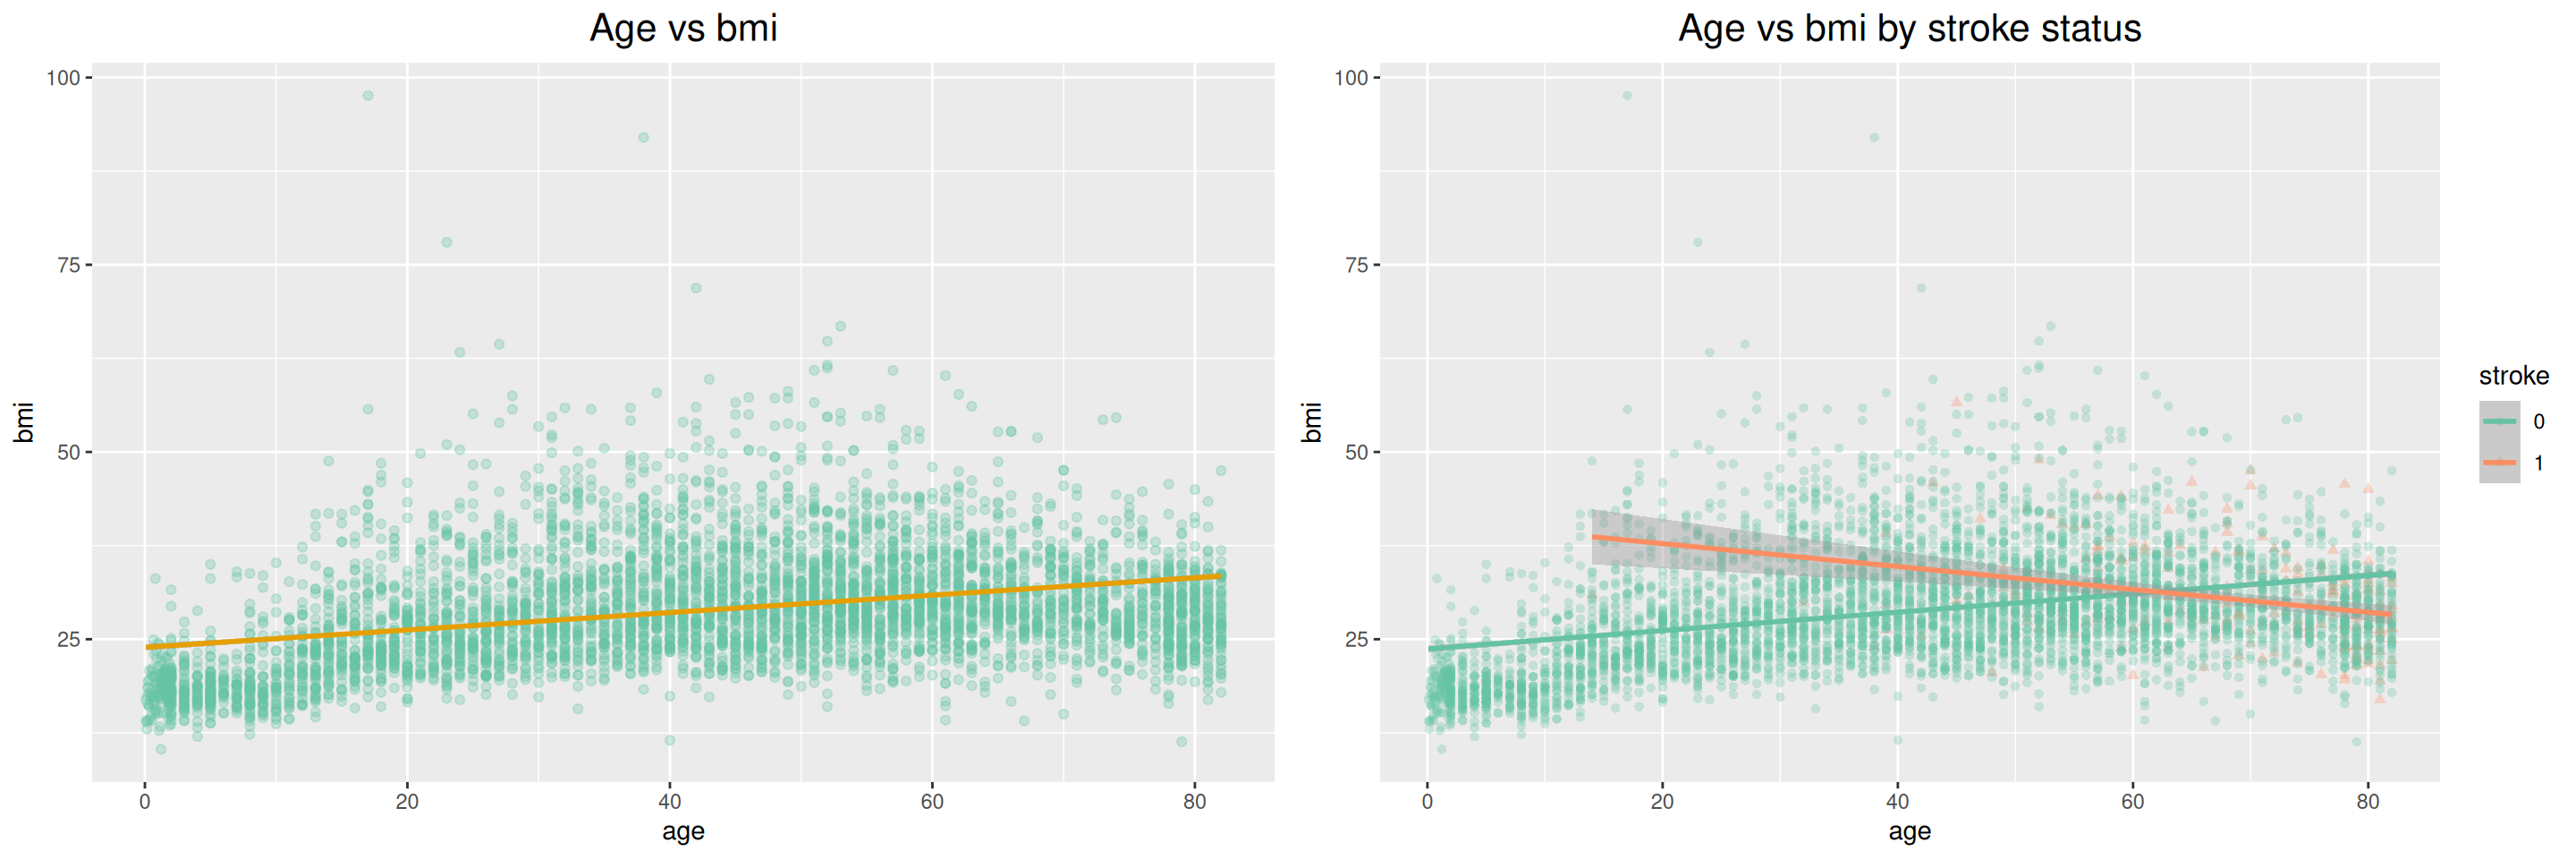
\includegraphics{Build-deploy-stroke-prediction-model-R_files/figure-latex/age_vs_bmi-1.pdf}

Is the interaction of age and stroke is statistically significant for
bmi?

We see the \textbf{body mass index on average increases by 0.12 units
with each additional year for non-stroke cases, but for stroke cases it
decreases by 0.12 - 0.2756 = -0.1556 for each additional year. However,
note that, age and stroke explains a very little variance in body mass
index: around \textasciitilde12 percent.}

\begin{Shaded}
\begin{Highlighting}[]
\NormalTok{lm\_mod }\OtherTok{\textless{}{-}} \FunctionTok{lm}\NormalTok{(bmi }\SpecialCharTok{\textasciitilde{}}\NormalTok{ age }\SpecialCharTok{*}\NormalTok{ stroke, }\AttributeTok{data =}\NormalTok{ dat)}
\FunctionTok{summary}\NormalTok{(lm\_mod)}
\end{Highlighting}
\end{Shaded}

\begin{verbatim}
## 
## Call:
## lm(formula = bmi ~ age * stroke, data = dat)
## 
## Residuals:
##     Min      1Q  Median      3Q     Max 
## -22.097  -4.998  -1.412   3.564  71.818 
## 
## Coefficients:
##              Estimate Std. Error t value Pr(>|t|)    
## (Intercept) 23.693664   0.228446 103.717  < 2e-16 ***
## age          0.122829   0.004827  25.446  < 2e-16 ***
## stroke1     17.125887   2.844665   6.020 1.87e-09 ***
## age:stroke1 -0.275655   0.041475  -6.646 3.33e-11 ***
## ---
## Signif. codes:  0 '***' 0.001 '**' 0.01 '*' 0.05 '.' 0.1 ' ' 1
## 
## Residual standard error: 7.368 on 4905 degrees of freedom
##   (201 observations effacées parce que manquantes)
## Multiple R-squared:  0.1204, Adjusted R-squared:  0.1198 
## F-statistic: 223.8 on 3 and 4905 DF,  p-value: < 2.2e-16
\end{verbatim}

\paragraph{\texorpdfstring{\textbf{Odds of stroke after adjusting for
all
variables}}{Odds of stroke after adjusting for all variables}}\label{odds-of-stroke-after-adjusting-for-all-variables}

Logistic regression models the log odds of stroke as a linear
combination of variables. It allows us to see the effect of each
covariate on the odds of stroke while adjusting for all the other
covariates. The result below shows that the age, average glucose level,
and hypertension are significant covariates for stroke, but heart
disease is not, after adjusting for other variables. In other words,
\textbf{older individuals, individuals with hypertension, and
individuals with higher glucose levels are at increased risk of stroke.}

\begin{Shaded}
\begin{Highlighting}[]
\NormalTok{lg\_model }\OtherTok{\textless{}{-}} \FunctionTok{glm}\NormalTok{(stroke }\SpecialCharTok{\textasciitilde{}}\NormalTok{ age }\SpecialCharTok{+}\NormalTok{ gender }\SpecialCharTok{+}\NormalTok{ hypertension }\SpecialCharTok{+}\NormalTok{ heart\_disease }\SpecialCharTok{+}\NormalTok{ ever\_married }\SpecialCharTok{+}\NormalTok{ work\_type }\SpecialCharTok{+}\NormalTok{ Residence\_type }\SpecialCharTok{+}\NormalTok{ avg\_glucose\_level  }\SpecialCharTok{+}\NormalTok{ smoking\_status, }\AttributeTok{data =}\NormalTok{ dat, }\AttributeTok{family =} \StringTok{"binomial"}\NormalTok{)}

\FunctionTok{summary}\NormalTok{(lg\_model)}
\end{Highlighting}
\end{Shaded}

\begin{verbatim}
## 
## Call:
## glm(formula = stroke ~ age + gender + hypertension + heart_disease + 
##     ever_married + work_type + Residence_type + avg_glucose_level + 
##     smoking_status, family = "binomial", data = dat)
## 
## Coefficients:
##                              Estimate Std. Error z value Pr(>|z|)    
## (Intercept)                -6.759e+00  7.527e-01  -8.980  < 2e-16 ***
## age                         7.464e-02  5.729e-03  13.029  < 2e-16 ***
## genderMale                  1.244e-02  1.418e-01   0.088 0.930114    
## genderOther                -1.054e+01  1.455e+03  -0.007 0.994221    
## hypertension1               4.050e-01  1.644e-01   2.463 0.013779 *  
## heart_disease1              2.791e-01  1.911e-01   1.461 0.144040    
## ever_marriedYes            -1.833e-01  2.254e-01  -0.814 0.415902    
## work_typeGovt_job          -9.298e-01  8.210e-01  -1.133 0.257393    
## work_typeNever_worked      -1.032e+01  3.095e+02  -0.033 0.973387    
## work_typePrivate           -7.877e-01  8.051e-01  -0.978 0.327907    
## work_typeSelf-employed     -1.165e+00  8.264e-01  -1.410 0.158683    
## Residence_typeUrban         8.334e-02  1.383e-01   0.602 0.546897    
## avg_glucose_level           4.053e-03  1.174e-03   3.451 0.000558 ***
## smoking_statusnever smoked -2.069e-01  1.759e-01  -1.176 0.239524    
## smoking_statussmokes        1.121e-01  2.153e-01   0.521 0.602553    
## smoking_statusUnknown      -7.298e-02  2.084e-01  -0.350 0.726145    
## ---
## Signif. codes:  0 '***' 0.001 '**' 0.01 '*' 0.05 '.' 0.1 ' ' 1
## 
## (Dispersion parameter for binomial family taken to be 1)
## 
##     Null deviance: 1990.4  on 5109  degrees of freedom
## Residual deviance: 1581.2  on 5094  degrees of freedom
## AIC: 1613.2
## 
## Number of Fisher Scoring iterations: 14
\end{verbatim}

To interpret the effect of age, hypertension, and average glucose level
on stroke, we need to exponentiate the coefficients. We see that
\textbf{each additional year is associated with the \textasciitilde7.7\%
increase in the odds of stroke. Each additional average glucose level is
associated with the \textasciitilde0.4\% increase in the odds of stroke.
People with hypertension have \textasciitilde1.5 times the odds of
stroke compared to those without hypertension.}

\begin{Shaded}
\begin{Highlighting}[]
\NormalTok{coeffs }\OtherTok{\textless{}{-}}\NormalTok{ lg\_model}\SpecialCharTok{$}\NormalTok{coefficients}

\NormalTok{coeffs\_sign }\OtherTok{\textless{}{-}}\NormalTok{ coeffs[}\FunctionTok{names}\NormalTok{(coeffs) }\SpecialCharTok{\%in\%} \FunctionTok{c}\NormalTok{(}\StringTok{"age"}\NormalTok{, }\StringTok{"hypertension1"}\NormalTok{, }\StringTok{"avg\_glucose\_level"}\NormalTok{)]}

\FunctionTok{exp}\NormalTok{(coeffs\_sign)}
\end{Highlighting}
\end{Shaded}

\begin{verbatim}
##               age     hypertension1 avg_glucose_level 
##          1.077495          1.499276          1.004061
\end{verbatim}

\section{Task Three: Evaluate and select prediction
models}\label{task-three-evaluate-and-select-prediction-models}

\subsubsection{\texorpdfstring{\textbf{First thing first: What
evaluation
measures?}}{First thing first: What evaluation measures?}}\label{first-thing-first-what-evaluation-measures}

This is a problem with high class imbalance: only around 5 percent of
observations are stroke cases. Thus it is important to choose relevant
evaluation measures. Without any learning, without even considering any
input variables, predicting no stroke would achieve a very high accuracy
result. Thus we concentrate on \textbf{sensitivity} and
\textbf{specificity} first. \textbf{Sensitivity measures the proportion
of individuals correctly identified as stroke cases among those who
actually have a stroke, and specificity measures the proportion of
individuals correctly identified as healthy among those who are actually
healthy.} These measures take values between O and 1. Now, if all
individuals are predicted as non-stroke ones, then the specificity will
be 1 since there is no false positives. However, sensitivity in this
case will be 0, since 0 stroke case, i.e., 0 true positive is
identified.

Sensitivity is also known as recall. Precision computes the fraction of
true positives over the sum of true and false positives. The
\textbf{F1-measure} is the harmonic mean of precision and recall, it
balances precision and recall. But notice that if the specificity is 1
and the sensitivity is 0, then the precision is undefined, since there
is neither true positives or false positives predicted. Thus, F1 measure
is not defined.

Next, we consider the \textbf{area under the ROC curve}. This curve
draws sensitivity against false positive rate (1-specificity) at every
cut-off threshold level for predicted probability values, and the larger
the area under this curve the better the predictive performance of
algorithm.

Finally, we consider \textbf{Matthews correlation coefficient. The value
of this metric is computed based on the entire confusion matrix, i.e.,
it takes into account true positives, false positives, true negatives
and false negatives. It can be considered the most suitable measure in
the class-imbalance setting.}

Now, since we are dealing with the class-imbalance problem, we can
choose cut-off threshold values below the standard 0.5 level. This will
output different values for sensitivity, specificity, F1-measure and
Matthews coefficient. Our strategy is based on the Youden's index, i.e.,
the threshold that maximizes sensitivity + specificity - 1.

\subsubsection{** Missing values, data
splitting**}\label{missing-values-data-splitting}

We can impute the missing values using the k-nearest neighbour method.
It means that the individuals having similar characteristics will have
similar body mass index. But it is questionable from precision medicine
point of view. We can as well remove these individuals from the data set
on the basis of biological differences between individuals even with
very similar characteristics.

We first split the data into the 75\%/25\% training and test sets using
rsample package of tidymodels framework. \textbf{We do stratification
based on the stroke variable to ensure that the proportion of stroke
cases is similar across these splits.} In what follow, we use set.seed
to ensure reproducibility.

\begin{Shaded}
\begin{Highlighting}[]
\FunctionTok{set.seed}\NormalTok{(}\DecValTok{123}\NormalTok{)}

\NormalTok{dat\_split }\OtherTok{\textless{}{-}} \FunctionTok{initial\_split}\NormalTok{(dat, }\AttributeTok{prop =} \DecValTok{3}\SpecialCharTok{/}\DecValTok{4}\NormalTok{, }\AttributeTok{strata =}\NormalTok{ stroke)}

\NormalTok{dat\_train }\OtherTok{\textless{}{-}} \FunctionTok{training}\NormalTok{(dat\_split)}

\NormalTok{dat\_test }\OtherTok{\textless{}{-}} \FunctionTok{testing}\NormalTok{(dat\_split)}
                      
\NormalTok{dat\_cv }\OtherTok{\textless{}{-}} \FunctionTok{vfold\_cv}\NormalTok{(dat\_train)}
\end{Highlighting}
\end{Shaded}

\subsubsection{\texorpdfstring{\textbf{Predictive
modeling}}{Predictive modeling}}\label{predictive-modeling}

We use logistic regression, also models of higher capacity, capable of
learning non-linear decision boundaries, such as random forest and an
improved version of the gradient boosting method, extreme gradient
boosting. The latter models are particularly suitable for data with many
categorical variables.

We train logistic regression with and without SMOTE. The latter
generates synthetic samples for the rare class based on the k-nearest
neighbour method. The proportion of synthetic examples can be controlled
thanks to the over\_ratio option in the recipe function. The number of
synthetic samples generated affect sensitivity and specificity: higher
number of synthetic samples will improve sensitivity, and degrade
specificity.

We use parsnip package of tidymodels to train logistic regression model
and random forest. There is no implementation of xgb in tidymodels, so
we use xgboost package. We do a grid search for hyperparameter tuning.

\paragraph{\texorpdfstring{\textbf{Logistic
regression}}{Logistic regression}}\label{logistic-regression}

\begin{Shaded}
\begin{Highlighting}[]
\NormalTok{ground\_truth }\OtherTok{\textless{}{-}} \FunctionTok{factor}\NormalTok{(dat\_test}\SpecialCharTok{$}\NormalTok{stroke, }\AttributeTok{levels =} \FunctionTok{c}\NormalTok{(}\DecValTok{1}\NormalTok{, }\DecValTok{0}\NormalTok{))}

\NormalTok{dat\_recipe }\OtherTok{\textless{}{-}} \FunctionTok{recipe}\NormalTok{(stroke }\SpecialCharTok{\textasciitilde{}}\NormalTok{ ., }\AttributeTok{data =}\NormalTok{ dat\_train) }\SpecialCharTok{\%\textgreater{}\%} \FunctionTok{step\_impute\_knn}\NormalTok{(}\FunctionTok{all\_predictors}\NormalTok{())}

\NormalTok{lr\_model }\OtherTok{\textless{}{-}} \FunctionTok{logistic\_reg}\NormalTok{() }\SpecialCharTok{\%\textgreater{}\%}  \FunctionTok{set\_engine}\NormalTok{(}\StringTok{"glm"}\NormalTok{) }\SpecialCharTok{\%\textgreater{}\%} \FunctionTok{set\_mode}\NormalTok{(}\StringTok{"classification"}\NormalTok{) }

\NormalTok{lr\_workflow }\OtherTok{\textless{}{-}} \FunctionTok{workflow}\NormalTok{() }\SpecialCharTok{\%\textgreater{}\%} \FunctionTok{add\_model}\NormalTok{(lr\_model) }\SpecialCharTok{\%\textgreater{}\%} \FunctionTok{add\_recipe}\NormalTok{(dat\_recipe)}

\NormalTok{lr\_fit }\OtherTok{\textless{}{-}} \FunctionTok{fit}\NormalTok{(lr\_workflow, }\AttributeTok{data =}\NormalTok{ dat\_train)}

\NormalTok{lr\_fit\_extracted }\OtherTok{\textless{}{-}} \FunctionTok{extract\_fit\_engine}\NormalTok{(lr\_fit)}

\NormalTok{lr\_probs1 }\OtherTok{\textless{}{-}} \FunctionTok{predict}\NormalTok{(lr\_fit, dat\_test, }\AttributeTok{type =} \StringTok{"prob"}\NormalTok{)}

\NormalTok{lr\_result1 }\OtherTok{\textless{}{-}} \FunctionTok{evaluate\_model\_fit}\NormalTok{(ground\_truth, lr\_probs1}\SpecialCharTok{$}\NormalTok{.pred\_1)}
\end{Highlighting}
\end{Shaded}

\begin{verbatim}
## Setting levels: control = 1, case = 0
\end{verbatim}

\begin{verbatim}
## Setting direction: controls > cases
\end{verbatim}

and with SMOTE:

\begin{Shaded}
\begin{Highlighting}[]
\NormalTok{dat\_smote\_recipe }\OtherTok{\textless{}{-}} \FunctionTok{recipe}\NormalTok{(stroke }\SpecialCharTok{\textasciitilde{}}\NormalTok{ ., }\AttributeTok{data =}\NormalTok{ dat\_train) }\SpecialCharTok{\%\textgreater{}\%}
  \FunctionTok{step\_impute\_knn}\NormalTok{(}\FunctionTok{all\_predictors}\NormalTok{()) }\SpecialCharTok{\%\textgreater{}\%}
  \FunctionTok{step\_dummy}\NormalTok{(}\FunctionTok{all\_nominal\_predictors}\NormalTok{()) }\SpecialCharTok{\%\textgreater{}\%} 
  \FunctionTok{step\_smote}\NormalTok{(stroke, }\AttributeTok{over\_ratio =} \FloatTok{0.5}\NormalTok{)}

\NormalTok{lr\_model2 }\OtherTok{\textless{}{-}} \FunctionTok{logistic\_reg}\NormalTok{() }\SpecialCharTok{\%\textgreater{}\%}  \FunctionTok{set\_engine}\NormalTok{(}\StringTok{"glm"}\NormalTok{) }\SpecialCharTok{\%\textgreater{}\%} \FunctionTok{set\_mode}\NormalTok{(}\StringTok{"classification"}\NormalTok{) }

\NormalTok{lr\_workflow2 }\OtherTok{\textless{}{-}} \FunctionTok{workflow}\NormalTok{() }\SpecialCharTok{\%\textgreater{}\%} \FunctionTok{add\_model}\NormalTok{(lr\_model2) }\SpecialCharTok{\%\textgreater{}\%} \FunctionTok{add\_recipe}\NormalTok{(dat\_smote\_recipe) }\DocumentationTok{\#\# use smote data recipe}

\NormalTok{lr\_fit2 }\OtherTok{\textless{}{-}} \FunctionTok{fit}\NormalTok{(lr\_workflow2, }\AttributeTok{data =}\NormalTok{ dat\_train)}

\NormalTok{lr\_fit\_extracted2 }\OtherTok{\textless{}{-}} \FunctionTok{extract\_fit\_engine}\NormalTok{(lr\_fit2)}

\NormalTok{lr\_probs2 }\OtherTok{\textless{}{-}} \FunctionTok{predict}\NormalTok{(lr\_fit2, dat\_test, }\AttributeTok{type =} \StringTok{"prob"}\NormalTok{)}

\NormalTok{lr\_result2 }\OtherTok{\textless{}{-}} \FunctionTok{evaluate\_model\_fit}\NormalTok{(ground\_truth, lr\_probs2}\SpecialCharTok{$}\NormalTok{.pred\_1)}
\end{Highlighting}
\end{Shaded}

\begin{verbatim}
## Setting levels: control = 1, case = 0
\end{verbatim}

\begin{verbatim}
## Setting direction: controls > cases
\end{verbatim}

\paragraph{\texorpdfstring{\textbf{Random
forest}}{Random forest}}\label{random-forest}

\begin{Shaded}
\begin{Highlighting}[]
\NormalTok{rf\_model }\OtherTok{\textless{}{-}} \FunctionTok{rand\_forest}\NormalTok{() }\SpecialCharTok{\%\textgreater{}\%} \FunctionTok{set\_args}\NormalTok{(}\AttributeTok{mtry =} \FunctionTok{tune}\NormalTok{()) }\SpecialCharTok{\%\textgreater{}\%}
  \FunctionTok{set\_engine}\NormalTok{(}\StringTok{"ranger"}\NormalTok{, }\AttributeTok{importance =} \StringTok{"impurity"}\NormalTok{) }\SpecialCharTok{\%\textgreater{}\%}
  \FunctionTok{set\_mode}\NormalTok{(}\StringTok{"classification"}\NormalTok{) }


\NormalTok{rf\_workflow }\OtherTok{\textless{}{-}} \FunctionTok{workflow}\NormalTok{() }\SpecialCharTok{\%\textgreater{}\%}
  \FunctionTok{add\_recipe}\NormalTok{(dat\_smote\_recipe) }\SpecialCharTok{\%\textgreater{}\%}
  \FunctionTok{add\_model}\NormalTok{(rf\_model)}

\NormalTok{rf\_grid }\OtherTok{\textless{}{-}} \FunctionTok{expand.grid}\NormalTok{(}\AttributeTok{mtry =} \FunctionTok{c}\NormalTok{(}\DecValTok{2}\NormalTok{, }\DecValTok{3}\NormalTok{, }\DecValTok{4}\NormalTok{, }\DecValTok{5}\NormalTok{))}

\NormalTok{rf\_tune\_results }\OtherTok{\textless{}{-}}\NormalTok{ rf\_workflow }\SpecialCharTok{\%\textgreater{}\%} \FunctionTok{tune\_grid}\NormalTok{(}\AttributeTok{resamples =}\NormalTok{ dat\_cv, }\AttributeTok{grid =}\NormalTok{ rf\_grid, }\AttributeTok{metrics =} \FunctionTok{metric\_set}\NormalTok{(roc\_auc))}

\NormalTok{rf\_tune\_results }\SpecialCharTok{\%\textgreater{}\%}  \FunctionTok{collect\_metrics}\NormalTok{()}
\end{Highlighting}
\end{Shaded}

\begin{verbatim}
## # A tibble: 4 x 7
##    mtry .metric .estimator  mean     n std_err .config             
##   <dbl> <chr>   <chr>      <dbl> <int>   <dbl> <chr>               
## 1     2 roc_auc binary     0.819    10 0.00867 Preprocessor1_Model1
## 2     3 roc_auc binary     0.817    10 0.0109  Preprocessor1_Model2
## 3     4 roc_auc binary     0.809    10 0.0116  Preprocessor1_Model3
## 4     5 roc_auc binary     0.808    10 0.0129  Preprocessor1_Model4
\end{verbatim}

\begin{Shaded}
\begin{Highlighting}[]
\NormalTok{param\_final }\OtherTok{\textless{}{-}}\NormalTok{ rf\_tune\_results }\SpecialCharTok{\%\textgreater{}\%} \FunctionTok{select\_best}\NormalTok{(}\AttributeTok{metric =} \StringTok{"roc\_auc"}\NormalTok{)}

\NormalTok{rf\_workflow }\OtherTok{\textless{}{-}}\NormalTok{ rf\_workflow }\SpecialCharTok{\%\textgreater{}\%} \FunctionTok{finalize\_workflow}\NormalTok{(param\_final)}

\NormalTok{rf\_fit }\OtherTok{\textless{}{-}}\NormalTok{ rf\_workflow }\SpecialCharTok{\%\textgreater{}\%} \FunctionTok{last\_fit}\NormalTok{(dat\_split)}

\CommentTok{\#test\_performance \textless{}{-} rf\_fit \%\textgreater{}\% collect\_metrics()}

\NormalTok{rf\_probs }\OtherTok{\textless{}{-}} \FunctionTok{as.data.frame}\NormalTok{(rf\_fit}\SpecialCharTok{$}\NormalTok{.predictions)}\SpecialCharTok{$}\NormalTok{.pred\_1}

\NormalTok{rf\_result }\OtherTok{\textless{}{-}} \FunctionTok{evaluate\_model\_fit}\NormalTok{(ground\_truth, rf\_probs)}
\end{Highlighting}
\end{Shaded}

\begin{verbatim}
## Setting levels: control = 1, case = 0
\end{verbatim}

\begin{verbatim}
## Setting direction: controls > cases
\end{verbatim}

\paragraph{\texorpdfstring{\textbf{Extreme gradient
boosting}}{Extreme gradient boosting}}\label{extreme-gradient-boosting}

\begin{Shaded}
\begin{Highlighting}[]
\NormalTok{dat\_smote\_recipe }\OtherTok{\textless{}{-}}\NormalTok{ dat\_smote\_recipe }\SpecialCharTok{\%\textgreater{}\%} \FunctionTok{prep}\NormalTok{()}

\NormalTok{X\_train }\OtherTok{\textless{}{-}}\NormalTok{ dat\_train }\SpecialCharTok{\%\textgreater{}\%} \FunctionTok{select}\NormalTok{(}\SpecialCharTok{{-}}\NormalTok{stroke)}
\NormalTok{X\_test }\OtherTok{\textless{}{-}}\NormalTok{ dat\_test }\SpecialCharTok{\%\textgreater{}\%} \FunctionTok{select}\NormalTok{(}\SpecialCharTok{{-}}\NormalTok{stroke)}

\NormalTok{X\_train }\OtherTok{\textless{}{-}} \FunctionTok{bake}\NormalTok{(dat\_smote\_recipe, X\_train)}
\NormalTok{X\_test }\OtherTok{\textless{}{-}} \FunctionTok{bake}\NormalTok{(dat\_smote\_recipe, X\_test)}

\NormalTok{y\_train }\OtherTok{\textless{}{-}} \FunctionTok{as.numeric}\NormalTok{(dat\_train}\SpecialCharTok{$}\NormalTok{stroke)}\SpecialCharTok{{-}}\DecValTok{1}
\NormalTok{y\_test  }\OtherTok{\textless{}{-}} \FunctionTok{as.numeric}\NormalTok{(dat\_test}\SpecialCharTok{$}\NormalTok{stroke)}\SpecialCharTok{{-}}\DecValTok{1}


\NormalTok{X\_train\_matrix }\OtherTok{\textless{}{-}} \FunctionTok{as.matrix}\NormalTok{(X\_train)}
\NormalTok{X\_test\_matrix }\OtherTok{\textless{}{-}} \FunctionTok{as.matrix}\NormalTok{(X\_test)}

\NormalTok{dtrain }\OtherTok{\textless{}{-}} \FunctionTok{xgb.DMatrix}\NormalTok{(}\AttributeTok{data =}\NormalTok{ X\_train\_matrix, }\AttributeTok{label =}\NormalTok{ y\_train)}
\NormalTok{dtest  }\OtherTok{\textless{}{-}} \FunctionTok{xgb.DMatrix}\NormalTok{(}\AttributeTok{data =}\NormalTok{ X\_test\_matrix, }\AttributeTok{label =}\NormalTok{ y\_test)}


\NormalTok{params\_list }\OtherTok{\textless{}{-}} \FunctionTok{expand.grid}\NormalTok{(}
  \AttributeTok{eta =} \FunctionTok{c}\NormalTok{(}\FloatTok{0.01}\NormalTok{, }\FloatTok{0.1}\NormalTok{, }\FloatTok{0.3}\NormalTok{),}
  \AttributeTok{max\_depth =} \FunctionTok{c}\NormalTok{(}\DecValTok{3}\NormalTok{, }\DecValTok{6}\NormalTok{, }\DecValTok{9}\NormalTok{, }\DecValTok{12}\NormalTok{),}
  \AttributeTok{subsample =} \FunctionTok{c}\NormalTok{(}\FloatTok{0.3}\NormalTok{, }\FloatTok{0.5}\NormalTok{, }\FloatTok{0.7}\NormalTok{, }\FloatTok{0.9}\NormalTok{),}
  \AttributeTok{colsample\_bytree =} \FunctionTok{c}\NormalTok{(}\FloatTok{0.2}\NormalTok{, }\FloatTok{0.5}\NormalTok{, }\FloatTok{0.8}\NormalTok{)}
\NormalTok{)}

\NormalTok{cv\_results }\OtherTok{\textless{}{-}} \FunctionTok{xgb\_tune}\NormalTok{(params\_list, dtrain, }\DecValTok{100}\NormalTok{)}

\NormalTok{cv\_summary }\OtherTok{\textless{}{-}} \FunctionTok{rbindlist}\NormalTok{(cv\_results)}

\NormalTok{best\_params }\OtherTok{\textless{}{-}}\NormalTok{ cv\_summary[}\FunctionTok{which.max}\NormalTok{(auc)]}

\DocumentationTok{\#\#\# we train xgb with the best hyperparameter configuration on the entire training set.}
\NormalTok{xgb\_final\_model }\OtherTok{\textless{}{-}} \FunctionTok{xgb.train}\NormalTok{(}
  \AttributeTok{params =} \FunctionTok{as.list}\NormalTok{(best\_params),}
  \AttributeTok{data =}\NormalTok{ dtrain,}
  \AttributeTok{nrounds =}\NormalTok{ best\_params}\SpecialCharTok{$}\NormalTok{best\_iteration,  }
  \AttributeTok{watchlist =} \FunctionTok{list}\NormalTok{(}\AttributeTok{train =}\NormalTok{ dtrain),}
  \AttributeTok{verbose =} \DecValTok{0}
\NormalTok{  )}
\end{Highlighting}
\end{Shaded}

\begin{verbatim}
## [15:44:03] WARNING: src/learner.cc:767: 
## Parameters: { "auc", "best_iteration" } are not used.
\end{verbatim}

\begin{Shaded}
\begin{Highlighting}[]
\NormalTok{xgb\_probs }\OtherTok{\textless{}{-}} \FunctionTok{predict}\NormalTok{(xgb\_final\_model, dtest)}

\NormalTok{xgb\_result }\OtherTok{\textless{}{-}} \FunctionTok{evaluate\_model\_fit}\NormalTok{(ground\_truth, xgb\_probs)}
\end{Highlighting}
\end{Shaded}

\begin{verbatim}
## Setting levels: control = 1, case = 0
\end{verbatim}

\begin{verbatim}
## Setting direction: controls > cases
\end{verbatim}

\subsubsection{\texorpdfstring{\textbf{Performance comparison of
models}}{Performance comparison of models}}\label{performance-comparison-of-models}

\textbf{According to Matthiews correlation coefficient, all methods
perform weakly (better than random)}. Their performances are comparable,
but logistic regression with smote stands out in terms of AUC,
F1-measure, Matthews coefficient and specificity. We see that generating
synthetic examples overall improved the predictive performance of
logistic regression model at the cost of sensitivity.

\begin{Shaded}
\begin{Highlighting}[]
\NormalTok{results\_df }\OtherTok{\textless{}{-}} \FunctionTok{tribble}\NormalTok{(}
  \SpecialCharTok{\textasciitilde{}}\NormalTok{Model,         }\SpecialCharTok{\textasciitilde{}}\NormalTok{Sensitivity, }\SpecialCharTok{\textasciitilde{}}\NormalTok{Specificity, }\SpecialCharTok{\textasciitilde{}}\NormalTok{F1,       }\SpecialCharTok{\textasciitilde{}}\NormalTok{AUC,      }\SpecialCharTok{\textasciitilde{}}\NormalTok{Matthews,}
  \StringTok{"Logistic Reg"}\NormalTok{, lr\_result1}\SpecialCharTok{$}\NormalTok{sensi, lr\_result1}\SpecialCharTok{$}\NormalTok{speci, lr\_result1}\SpecialCharTok{$}\NormalTok{f1, lr\_result1}\SpecialCharTok{$}\NormalTok{aucroc, lr\_result1}\SpecialCharTok{$}\NormalTok{matcc,}
  \StringTok{"Logistic Reg Smote"}\NormalTok{, lr\_result2}\SpecialCharTok{$}\NormalTok{sensi, lr\_result2}\SpecialCharTok{$}\NormalTok{speci, lr\_result2}\SpecialCharTok{$}\NormalTok{f1, lr\_result2}\SpecialCharTok{$}\NormalTok{aucroc, lr\_result2}\SpecialCharTok{$}\NormalTok{matcc,}
  \StringTok{"Random Forest Smote"}\NormalTok{, rf\_result}\SpecialCharTok{$}\NormalTok{sensi, rf\_result}\SpecialCharTok{$}\NormalTok{speci, rf\_result}\SpecialCharTok{$}\NormalTok{f1, rf\_result}\SpecialCharTok{$}\NormalTok{aucroc, rf\_result}\SpecialCharTok{$}\NormalTok{matcc,}
  \StringTok{"XGBoost Smote"}\NormalTok{,       xgb\_result}\SpecialCharTok{$}\NormalTok{sensi, xgb\_result}\SpecialCharTok{$}\NormalTok{speci, xgb\_result}\SpecialCharTok{$}\NormalTok{f1, xgb\_result}\SpecialCharTok{$}\NormalTok{aucroc, xgb\_result}\SpecialCharTok{$}\NormalTok{matcc}
\NormalTok{)}


\NormalTok{results\_long }\OtherTok{\textless{}{-}}\NormalTok{ results\_df }\SpecialCharTok{\%\textgreater{}\%} \FunctionTok{pivot\_longer}\NormalTok{(}\AttributeTok{cols =} \SpecialCharTok{{-}}\NormalTok{Model, }\AttributeTok{names\_to =} \StringTok{"Metric"}\NormalTok{, }\AttributeTok{values\_to =} \StringTok{"Value"}\NormalTok{)}


\FunctionTok{ggplot}\NormalTok{(results\_long, }\FunctionTok{aes}\NormalTok{(}\AttributeTok{x =}\NormalTok{ Metric, }\AttributeTok{y =}\NormalTok{ Value, }\AttributeTok{fill =}\NormalTok{ Model)) }\SpecialCharTok{+}
  \FunctionTok{geom\_bar}\NormalTok{(}\AttributeTok{stat =} \StringTok{"identity"}\NormalTok{, }\AttributeTok{position =} \FunctionTok{position\_dodge}\NormalTok{(), }\AttributeTok{width =} \FloatTok{0.7}\NormalTok{) }\SpecialCharTok{+}
  \FunctionTok{scale\_fill\_brewer}\NormalTok{(}\AttributeTok{palette =} \StringTok{"Set2"}\NormalTok{) }\SpecialCharTok{+}
  \FunctionTok{scale\_color\_brewer}\NormalTok{(}\AttributeTok{palette =} \StringTok{"Set2"}\NormalTok{) }\SpecialCharTok{+}
  \FunctionTok{labs}\NormalTok{(}
    \AttributeTok{title =} \StringTok{"Performance comparison"}\NormalTok{,}
    \AttributeTok{y =} \StringTok{"Value"}\NormalTok{,}
    \AttributeTok{x =} \StringTok{""}
\NormalTok{  ) }\SpecialCharTok{+}
  \FunctionTok{theme\_minimal}\NormalTok{()}\SpecialCharTok{+}     
  \FunctionTok{theme}\NormalTok{(}\AttributeTok{plot.title =} \FunctionTok{element\_text}\NormalTok{(}\AttributeTok{hjust =} \FloatTok{0.5}\NormalTok{, }\AttributeTok{size =} \DecValTok{16}\NormalTok{))}
\end{Highlighting}
\end{Shaded}

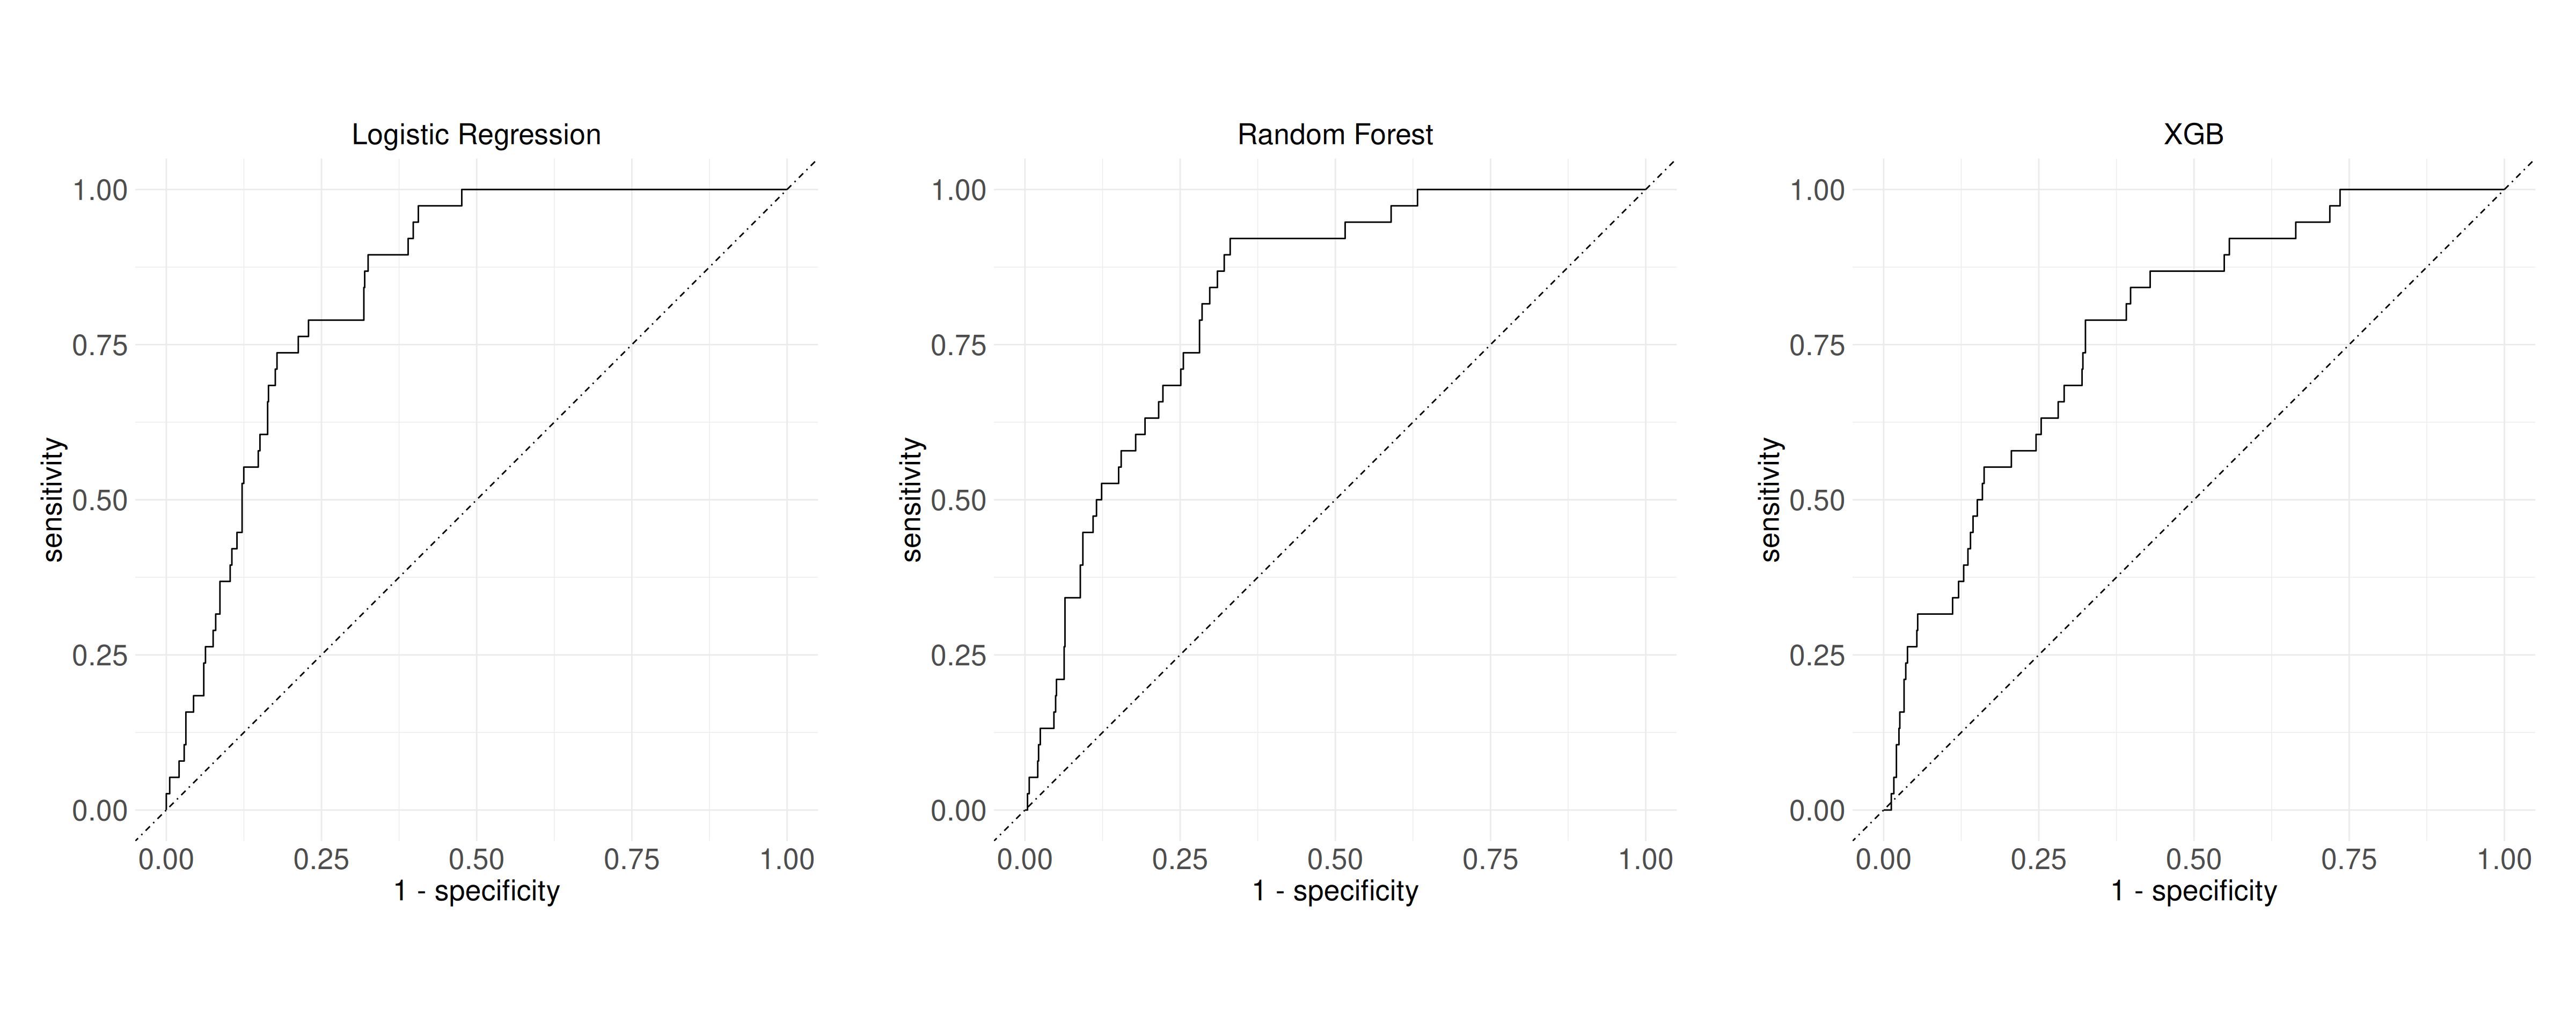
\includegraphics{Build-deploy-stroke-prediction-model-R_files/figure-latex/unnamed-chunk-15-1.pdf}

\begin{Shaded}
\begin{Highlighting}[]
\NormalTok{p1 }\OtherTok{\textless{}{-}} \FunctionTok{plot\_roc}\NormalTok{(}\FunctionTok{data.frame}\NormalTok{(ground\_truth, }\AttributeTok{probs=}\NormalTok{lr\_probs2}\SpecialCharTok{$}\NormalTok{.pred\_1), }\StringTok{"Logistic Regression"}\NormalTok{)}

\NormalTok{p2 }\OtherTok{\textless{}{-}}  \FunctionTok{plot\_roc}\NormalTok{(}\FunctionTok{data.frame}\NormalTok{(ground\_truth, }\AttributeTok{probs=}\NormalTok{rf\_probs), }\StringTok{"Random Forest"}\NormalTok{)}

\NormalTok{p3 }\OtherTok{\textless{}{-}}  \FunctionTok{plot\_roc}\NormalTok{(}\FunctionTok{data.frame}\NormalTok{(ground\_truth, }\AttributeTok{probs=}\NormalTok{xgb\_probs), }\StringTok{"XGB"}\NormalTok{)}

\FunctionTok{grid.arrange}\NormalTok{(p1, p2, p3, }\AttributeTok{ncol =} \DecValTok{4}\NormalTok{)}
\end{Highlighting}
\end{Shaded}

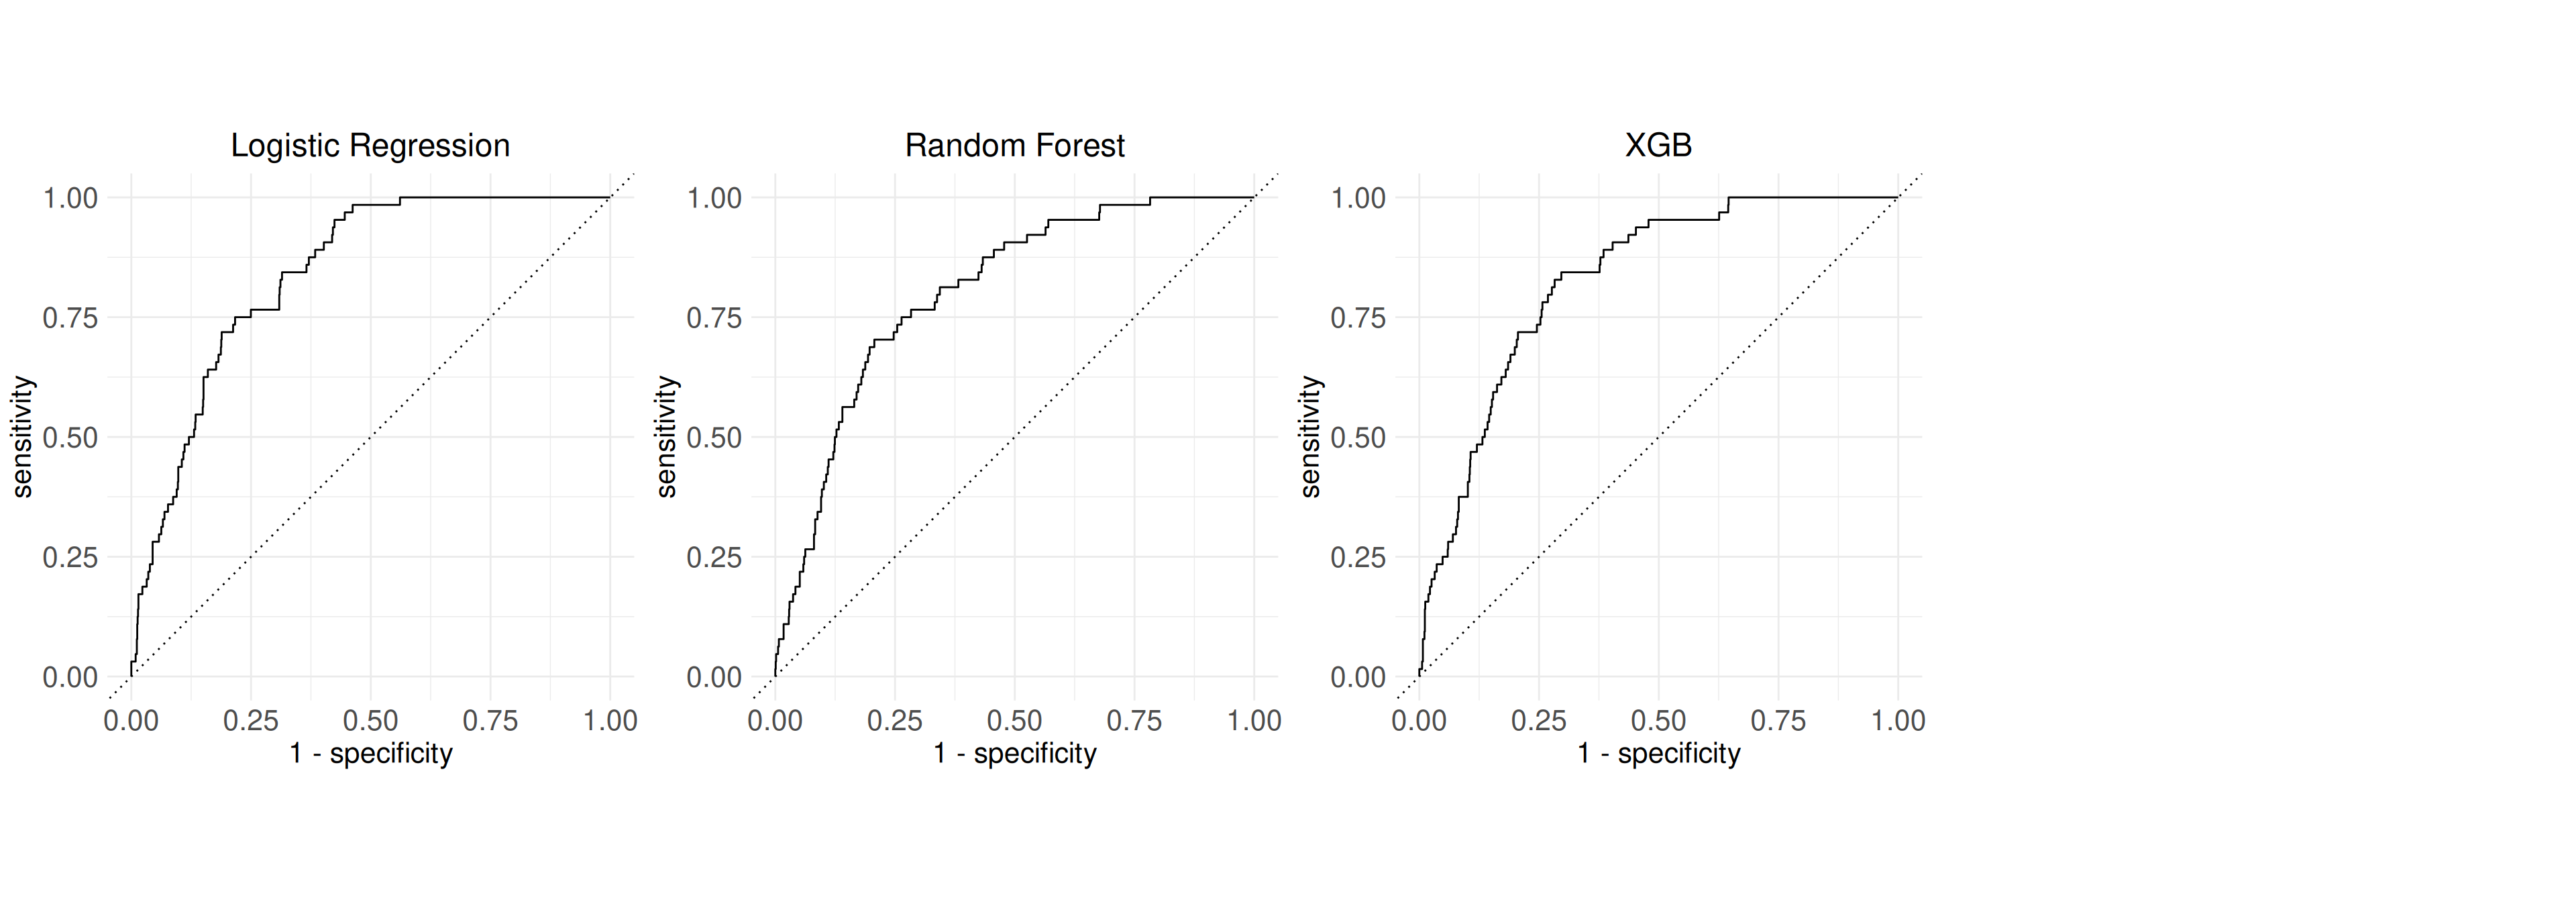
\includegraphics{Build-deploy-stroke-prediction-model-R_files/figure-latex/unnamed-chunk-16-1.pdf}

From the confusion matrix, we see that a lot of individuals are
predicted as the stroke case, since we chose lower cut-off threshold
from the ROC curve. Logistic regression has smaller number of false
positives.

\begin{Shaded}
\begin{Highlighting}[]
\NormalTok{p1 }\OtherTok{\textless{}{-}} \FunctionTok{plot\_confusion\_matrix}\NormalTok{(ground\_truth, lr\_result2}\SpecialCharTok{$}\NormalTok{pred\_class, }\FunctionTok{round}\NormalTok{(lr\_result2}\SpecialCharTok{$}\NormalTok{matcc, }\DecValTok{2}\NormalTok{), }\StringTok{"Logistic regression"}\NormalTok{)}

\NormalTok{p2 }\OtherTok{\textless{}{-}} \FunctionTok{plot\_confusion\_matrix}\NormalTok{(ground\_truth, rf\_result}\SpecialCharTok{$}\NormalTok{pred\_class, }\FunctionTok{round}\NormalTok{(rf\_result}\SpecialCharTok{$}\NormalTok{matcc, }\DecValTok{2}\NormalTok{), }\StringTok{"Random forest"}\NormalTok{)}

\NormalTok{p3 }\OtherTok{\textless{}{-}} \FunctionTok{plot\_confusion\_matrix}\NormalTok{(ground\_truth, xgb\_result}\SpecialCharTok{$}\NormalTok{pred\_class, }\FunctionTok{round}\NormalTok{(xgb\_result}\SpecialCharTok{$}\NormalTok{matcc, }\DecValTok{2}\NormalTok{), }\StringTok{"XGB"}\NormalTok{)}


\FunctionTok{grid.arrange}\NormalTok{(p1, p2, p3, }\AttributeTok{ncol =} \DecValTok{3}\NormalTok{)}
\end{Highlighting}
\end{Shaded}

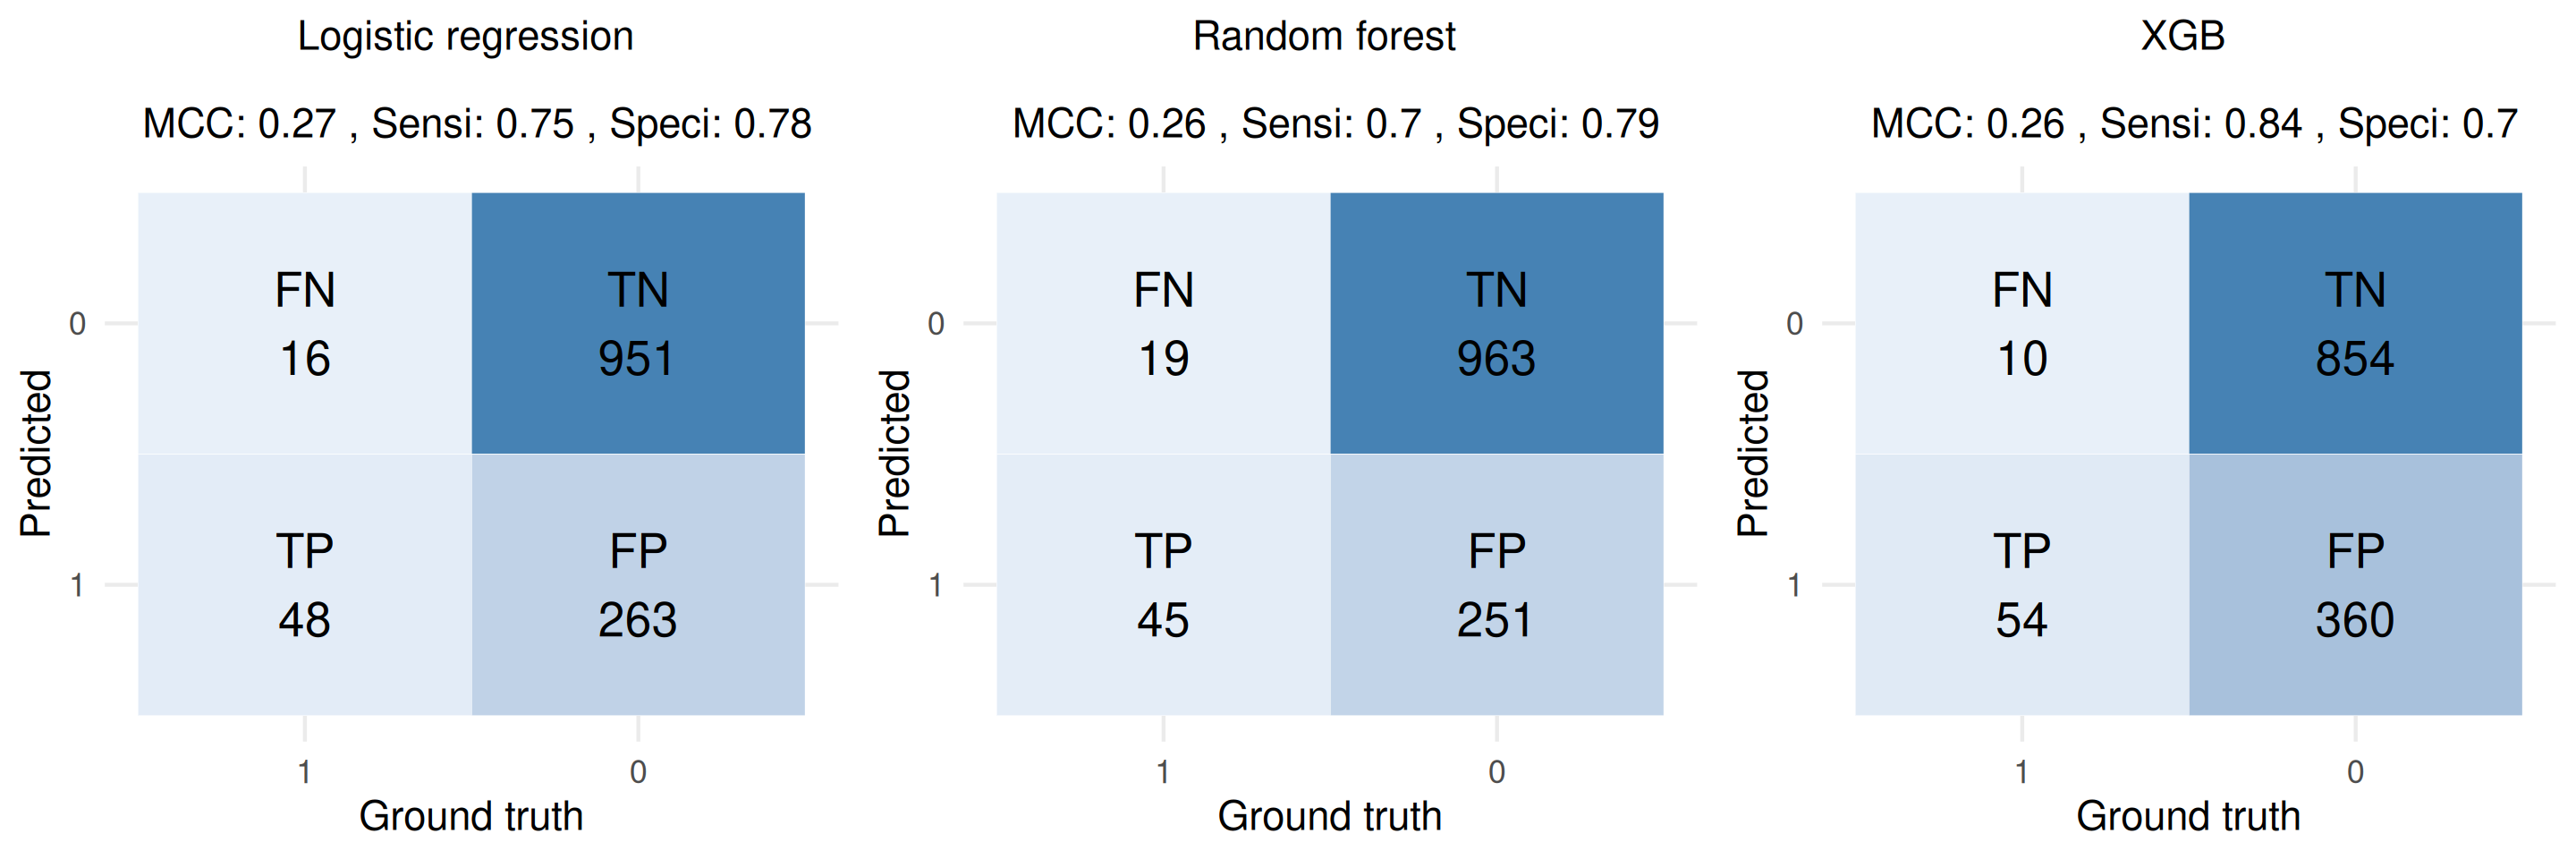
\includegraphics{Build-deploy-stroke-prediction-model-R_files/figure-latex/unnamed-chunk-17-1.pdf}

\subsubsection{\texorpdfstring{\textbf{False positives and false
negatives of logistic
regression}}{False positives and false negatives of logistic regression}}\label{false-positives-and-false-negatives-of-logistic-regression}

Now let us look at the distribution of incorrect predictions for
logistic regression (trained with smote). We consider important
variables such as age and average glucose level. Since age is a very
important risk factor for stroke, as expected, there are many false
positives for older age. There are many false postivies across all
values of average glucose but they are mostly concetrated around its two
modes.

\begin{Shaded}
\begin{Highlighting}[]
\NormalTok{preds }\OtherTok{\textless{}{-}}\NormalTok{ lr\_result2}\SpecialCharTok{$}\NormalTok{pred\_class}

\NormalTok{dat\_test\_preds }\OtherTok{\textless{}{-}}\NormalTok{ dat\_test}

\NormalTok{dat\_test\_preds}\SpecialCharTok{$}\NormalTok{preds }\OtherTok{\textless{}{-}} \FunctionTok{factor}\NormalTok{(preds, }\AttributeTok{levels=}\FunctionTok{c}\NormalTok{(}\DecValTok{1}\NormalTok{,}\DecValTok{0}\NormalTok{))}

\NormalTok{dat\_test\_preds}\SpecialCharTok{$}\NormalTok{outcome }\OtherTok{\textless{}{-}} \FunctionTok{with}\NormalTok{(dat\_test\_preds, }\FunctionTok{ifelse}\NormalTok{(}
\NormalTok{  stroke }\SpecialCharTok{==} \DecValTok{1} \SpecialCharTok{\&}\NormalTok{ preds }\SpecialCharTok{==} \DecValTok{1}\NormalTok{, }\StringTok{"True Positive"}\NormalTok{,}
  \FunctionTok{ifelse}\NormalTok{(stroke }\SpecialCharTok{==} \DecValTok{0} \SpecialCharTok{\&}\NormalTok{ preds }\SpecialCharTok{==} \DecValTok{0}\NormalTok{, }\StringTok{"True Negative"}\NormalTok{,}
  \FunctionTok{ifelse}\NormalTok{(stroke }\SpecialCharTok{==} \DecValTok{0} \SpecialCharTok{\&}\NormalTok{ preds }\SpecialCharTok{==} \DecValTok{1}\NormalTok{, }\StringTok{"False Positive"}\NormalTok{, }\StringTok{"False Negative"}\NormalTok{))))}


\NormalTok{p1 }\OtherTok{\textless{}{-}} \FunctionTok{ggplot}\NormalTok{(dat\_test\_preds, }\FunctionTok{aes}\NormalTok{(}\AttributeTok{x =}\NormalTok{ avg\_glucose\_level, }\AttributeTok{fill =} \FunctionTok{factor}\NormalTok{(stroke))) }\SpecialCharTok{+}
  \FunctionTok{geom\_density}\NormalTok{(}\AttributeTok{alpha =} \FloatTok{0.4}\NormalTok{) }\SpecialCharTok{+}
  
  \CommentTok{\# Rug plot for incorrect predictions}
  \FunctionTok{geom\_rug}\NormalTok{(}\AttributeTok{data =} \FunctionTok{subset}\NormalTok{(dat\_test\_preds, outcome }\SpecialCharTok{\%in\%} \FunctionTok{c}\NormalTok{(}\StringTok{"False Positive"}\NormalTok{, }\StringTok{"False Negative"}\NormalTok{)),}
           \FunctionTok{aes}\NormalTok{(}\AttributeTok{color =}\NormalTok{ outcome),}
           \AttributeTok{sides =} \StringTok{"b"}\NormalTok{, }\AttributeTok{alpha =} \FloatTok{0.7}\NormalTok{) }\SpecialCharTok{+}
  
  \CommentTok{\# Manual fill colors for stroke = 0 and 1}
  \FunctionTok{scale\_fill\_manual}\NormalTok{(}\AttributeTok{values =} \FunctionTok{c}\NormalTok{(}\StringTok{"0"} \OtherTok{=} \StringTok{"\#A6CEE3"}\NormalTok{, }\StringTok{"1"} \OtherTok{=} \StringTok{"\#33A02C"}\NormalTok{),}
                    \AttributeTok{labels =} \FunctionTok{c}\NormalTok{(}\StringTok{"No Stroke"}\NormalTok{, }\StringTok{"Stroke"}\NormalTok{),}
                    \AttributeTok{name =} \StringTok{"Stroke Status"}\NormalTok{) }\SpecialCharTok{+}
  
  \CommentTok{\# Manual colors for rug (incorrect predictions)}
  \FunctionTok{scale\_color\_manual}\NormalTok{(}\AttributeTok{values =} \FunctionTok{c}\NormalTok{(}\StringTok{"False Positive"} \OtherTok{=} \StringTok{"blue"}\NormalTok{, }\StringTok{"False Negative"} \OtherTok{=} \StringTok{"red"}\NormalTok{),}
                     \AttributeTok{name =} \StringTok{"Incorrect Prediction"}\NormalTok{) }\SpecialCharTok{+}

  \FunctionTok{labs}\NormalTok{(}\AttributeTok{x =} \StringTok{"Average glucose level"}\NormalTok{, }\AttributeTok{y =} \StringTok{"Density"}\NormalTok{) }\SpecialCharTok{+}
  \FunctionTok{theme\_minimal}\NormalTok{(}\AttributeTok{base\_size =} \DecValTok{14}\NormalTok{)}



\NormalTok{p2 }\OtherTok{\textless{}{-}} \FunctionTok{ggplot}\NormalTok{(dat\_test\_preds, }\FunctionTok{aes}\NormalTok{(}\AttributeTok{x =}\NormalTok{ age, }\AttributeTok{fill =} \FunctionTok{factor}\NormalTok{(stroke))) }\SpecialCharTok{+}
  \FunctionTok{geom\_density}\NormalTok{(}\AttributeTok{alpha =} \FloatTok{0.4}\NormalTok{) }\SpecialCharTok{+}
  
  \CommentTok{\# Rug plot for incorrect predictions}
  \FunctionTok{geom\_rug}\NormalTok{(}\AttributeTok{data =} \FunctionTok{subset}\NormalTok{(dat\_test\_preds, outcome }\SpecialCharTok{\%in\%} \FunctionTok{c}\NormalTok{(}\StringTok{"False Positive"}\NormalTok{, }\StringTok{"False Negative"}\NormalTok{)),}
           \FunctionTok{aes}\NormalTok{(}\AttributeTok{color =}\NormalTok{ outcome),}
           \AttributeTok{sides =} \StringTok{"b"}\NormalTok{, }\AttributeTok{alpha =} \FloatTok{0.7}\NormalTok{) }\SpecialCharTok{+}
  
  \CommentTok{\# Manual fill colors for stroke = 0 and 1}
  \FunctionTok{scale\_fill\_manual}\NormalTok{(}\AttributeTok{values =} \FunctionTok{c}\NormalTok{(}\StringTok{"0"} \OtherTok{=} \StringTok{"\#A6CEE3"}\NormalTok{, }\StringTok{"1"} \OtherTok{=} \StringTok{"\#33A02C"}\NormalTok{),}
                    \AttributeTok{labels =} \FunctionTok{c}\NormalTok{(}\StringTok{"No Stroke"}\NormalTok{, }\StringTok{"Stroke"}\NormalTok{),}
                    \AttributeTok{name =} \StringTok{"Stroke Status"}\NormalTok{) }\SpecialCharTok{+}
  
  \CommentTok{\# Manual colors for rug (incorrect predictions)}
  \FunctionTok{scale\_color\_manual}\NormalTok{(}\AttributeTok{values =} \FunctionTok{c}\NormalTok{(}\StringTok{"False Positive"} \OtherTok{=} \StringTok{"blue"}\NormalTok{, }\StringTok{"False Negative"} \OtherTok{=} \StringTok{"red"}\NormalTok{),}
                     \AttributeTok{name =} \StringTok{"Incorrect Prediction"}\NormalTok{) }\SpecialCharTok{+}

  \FunctionTok{labs}\NormalTok{(}\AttributeTok{x =} \StringTok{"Age"}\NormalTok{, }\AttributeTok{y =} \StringTok{"Density"}\NormalTok{) }\SpecialCharTok{+}
  \FunctionTok{theme\_minimal}\NormalTok{(}\AttributeTok{base\_size =} \DecValTok{14}\NormalTok{)}

\FunctionTok{grid.arrange}\NormalTok{(p1, p2, }\AttributeTok{ncol=}\DecValTok{2}\NormalTok{)}
\end{Highlighting}
\end{Shaded}

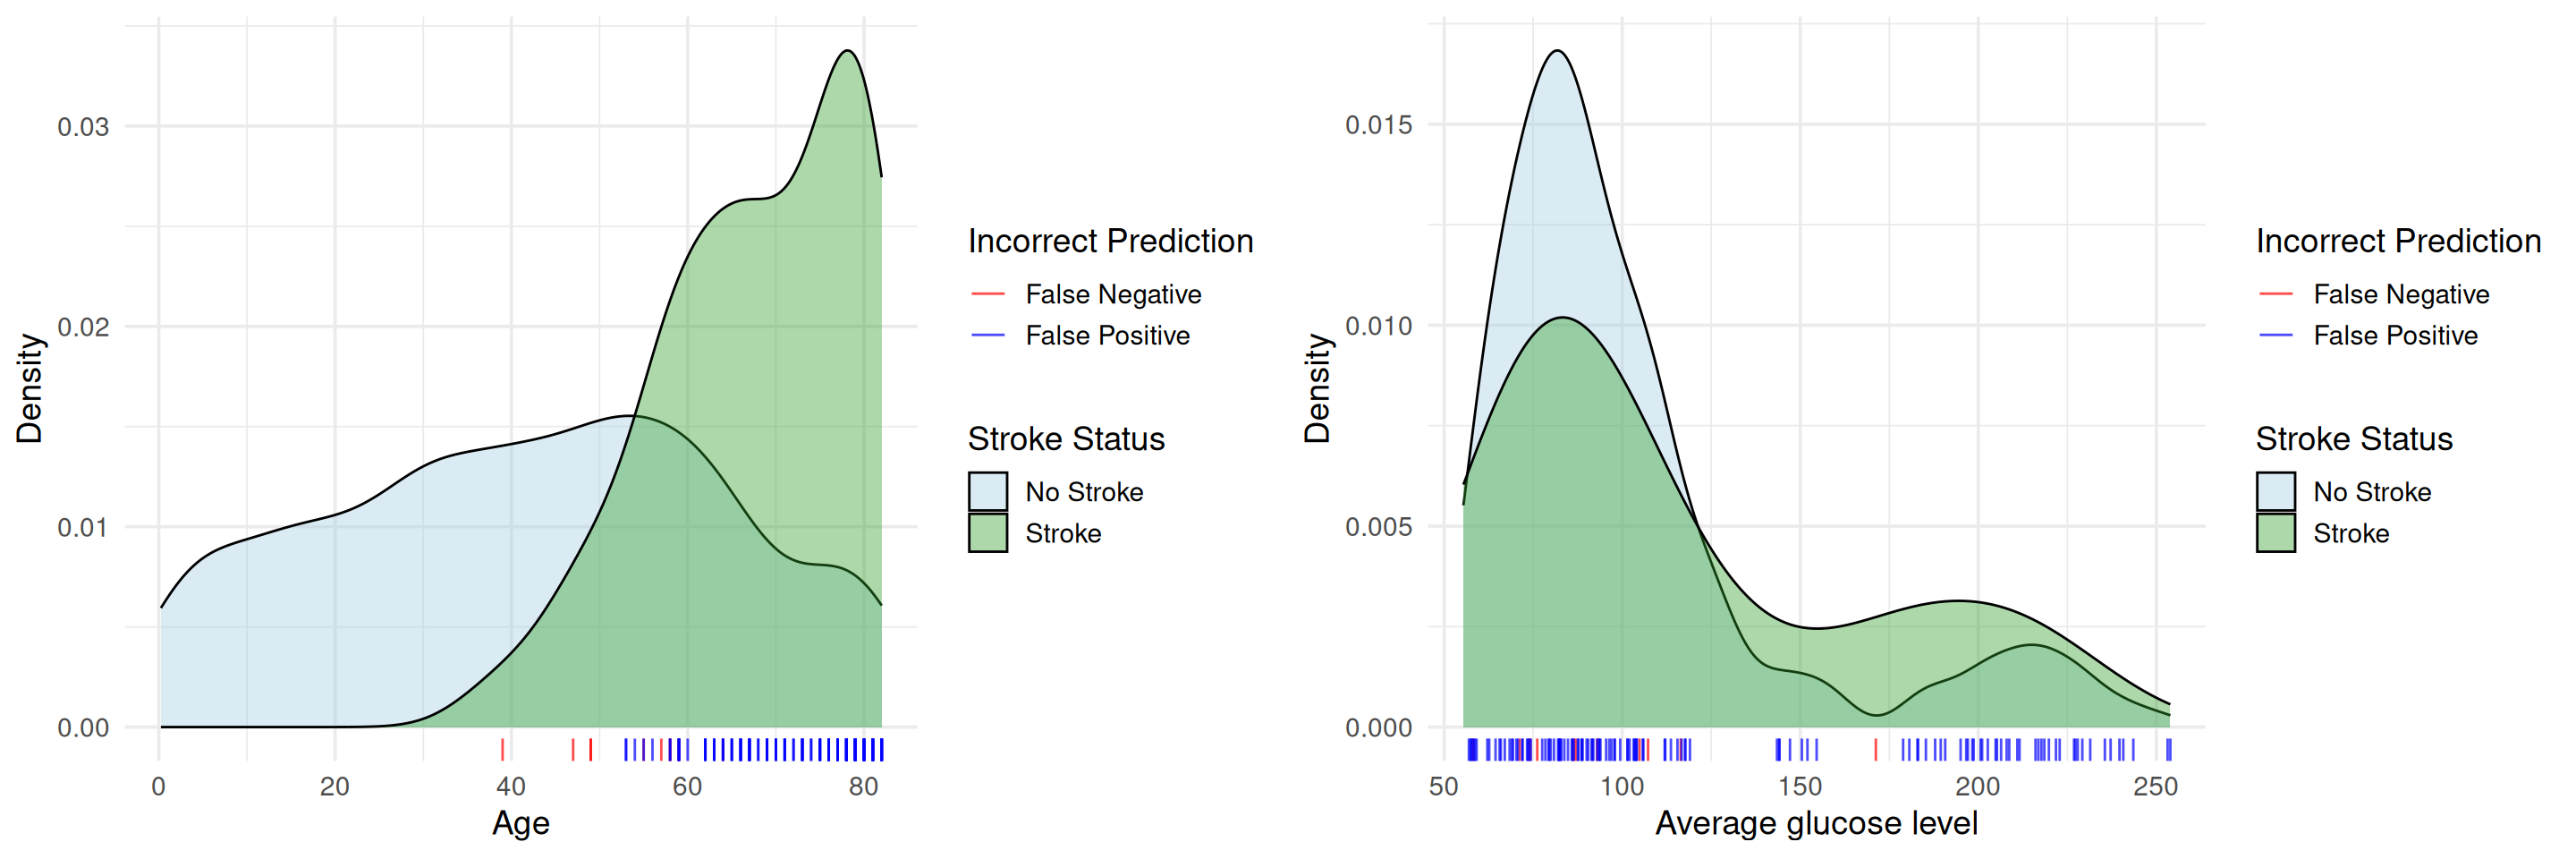
\includegraphics{Build-deploy-stroke-prediction-model-R_files/figure-latex/incorrect-preds-1.pdf}

\section{Task Four: Deploy the prediction
model}\label{task-four-deploy-the-prediction-model}

For deployment, we train logistic regression on the entire dataset,
where we impute the missing values of BMI and generate synthetic
examples of the rare class.

\begin{Shaded}
\begin{Highlighting}[]
\NormalTok{final\_data }\OtherTok{\textless{}{-}}\NormalTok{ dat}

\NormalTok{final\_recipe }\OtherTok{\textless{}{-}} \FunctionTok{recipe}\NormalTok{(stroke }\SpecialCharTok{\textasciitilde{}}\NormalTok{ ., }\AttributeTok{data =}\NormalTok{ final\_data) }\SpecialCharTok{\%\textgreater{}\%}
  \FunctionTok{step\_impute\_knn}\NormalTok{(}\FunctionTok{all\_predictors}\NormalTok{()) }\SpecialCharTok{\%\textgreater{}\%}
  \FunctionTok{step\_dummy}\NormalTok{(}\FunctionTok{all\_nominal\_predictors}\NormalTok{()) }\SpecialCharTok{\%\textgreater{}\%} 
  \FunctionTok{step\_smote}\NormalTok{(stroke, }\AttributeTok{over\_ratio =} \FloatTok{0.5}\NormalTok{)}


\NormalTok{final\_workflow }\OtherTok{\textless{}{-}} \FunctionTok{workflow}\NormalTok{() }\SpecialCharTok{\%\textgreater{}\%} 
  \FunctionTok{add\_model}\NormalTok{(lr\_model2) }\SpecialCharTok{\%\textgreater{}\%} 
  \FunctionTok{add\_recipe}\NormalTok{(final\_recipe)}


\NormalTok{final\_fit }\OtherTok{\textless{}{-}} \FunctionTok{fit}\NormalTok{(final\_workflow, }\AttributeTok{data =}\NormalTok{ final\_data)}

\FunctionTok{saveRDS}\NormalTok{(final\_fit, }\AttributeTok{file =} \StringTok{"stroke\_model.rds"}\NormalTok{)}
\end{Highlighting}
\end{Shaded}

\section{Task Five: Findings and
Conclusions}\label{task-five-findings-and-conclusions}

The prevalence of stroke cases is approximately 5\%, making this a
highly imbalanced dataset from a classification perspective. Data
visualization revealed considerable overlap between the
class-conditional distributions of key variables such as body mass
index, average glucose level, heart disease, and age. This indicates
that no single covariate is clearly discriminative for stroke
classification.

Statistical analysis confirmed that age is a particularly important risk
factor: the majority of stroke cases occur above the age of
\textasciitilde60. Other significant predictors include hypertension and
average glucose level. In contrast, gender does not appear to play a
substantial role, with stroke occurring at similar rates across male and
female individuals.

To address class imbalance problem, we applied SMOTE to synthetically
generate examples of the stroke class and we used a lower-than-standard
probability threshold (less than 0.5) to classify strokes. These
manipulations increase model sensitivity at the cost of more false
positives. We used a parametric method such as logistic regression, and
tree-based models capable of learning highly non-linear decision
boundaries and well adapted to data with many categorical variable:
random forest and gradient boosting. All models are comparable regarding
their predictive performance: they are better than a random guess
according to Matthews correlation coefficient which is computed based on
the whole confusion matrix. However logistic regression stood out with
respect to AUC, F1 measures, Matthews correlation coefficient and
specificity.

There is a clear trade-off between sensitivity and specificity:
improving sensitivity inevitably results in more false positives and
some false negatives. For example, adjusting the classification
threshold alters the balance between these metrics. This is an important
epidemiological question: what are the consequences of generating many
false positives in order to detect a rare but serious condition like
stroke?

\end{document}
